%%%%%%%%%%%%%%%%%%%%%%%%%%%%%%%%%%%%%%%%%%%%%%%%%%%%%%%%%%%%%%%%%%%%%%%%%%%%%%%%%%%%%%%%%%%%%%%%%%%%%%%%%%
%Write by:ShuwenHe
%Date:20230613
%%%%%%%%%%%%%%%%%%%%%%%%%%%%%%%%%%%%%%%%%%%%%%%%%%%%%%%%%%%%%%%%%%%%%%%%%%%%%%%%%%%%%%%%%%%%%%%%%%%%%%%%%%

%%%%%%%%%%%%%%%%%%%%%%%%%%%%%%%%%%%%%%%%%%%%%%%%%%%%%%%%%%%%%%%%%%%%%%%%%%%%%%%%%%%%%%%%%%%%%%%%%%%%%%%%%%
\documentclass[12pt,twiside,a4paper]{ctexbook}
\usepackage[centertags]{amsmath}
\usepackage{amsfonts}
\usepackage{amsthm}
\usepackage{newlfont}
\usepackage{makeidx}
\usepackage{wasysym}
\usepackage{geometry} 
\usepackage{graphics}
\usepackage{slashbox} 
\usepackage{fancyhdr} 
\usepackage[pdftex]{graphicx}
\usepackage{epstopdf}
\usepackage{cite}
\usepackage{listings}
\usepackage{tocbibind}
\usepackage{ulem} %
\usepackage[numbers,sort&compress]{natbib}

\setlength\parskip{\baselineskip}
\setcounter{tocdepth}{9} % 生成目录层级
\setcounter{secnumdepth}{5}
\renewcommand\thesection{\arabic{section}}
\usepackage[pdfstartview=FitH,CJKbookmarks=true,bookmarks,bookmarksnumbered=true,
    colorlinks=true,citecolor=black,linkcolor=black,anchorcolor=green,urlcolor=black]{hyperref}
\usepackage{titlesec}
\titleformat{\chapter}[display]{\normalfont\huge\bfseries\center}{\chaptertitlename}{1pt}{\Huge}

\titleformat{\section}{\normalfont\Large\bfseries}{\thesection}{1em}{}
\titlespacing*{\section} {0pt}{0.5ex plus 1ex minus .2ex}{0.3ex plus .2ex}

\titleformat{\subsection}{\normalfont\large\bfseries}{\thesubsection}{1em}{}
\titlespacing*{\subsection} {0pt}{0.25ex plus 1ex minus .1ex}{0.5ex plus .1ex}

\titleformat{\subsubsection}{\normalfont\normalsize\bfseries}{\thesubsubsection}{1em}{}
\titlespacing*{\subsubsection}{0pt}{3.25ex plus 1ex minus .2ex}{1.5ex plus .2ex}


\titleformat{\paragraph}[runin]{\normalfont\normalsize\bfseries}{\theparagraph}{1em}{}
\titlespacing*{\chapter} {0pt}{10pt}{10pt}

\titlespacing*{\paragraph} {0pt}{3.25ex plus 1ex minus .2ex}{1em}
\titleformat{\subparagraph}[runin]{\normalfont\normalsize\bfseries}{\thesubparagraph}{1em}{}

\titlespacing*{\subparagraph} {\parindent}{3.25ex plus 1ex minus .2ex}{1em}
\numberwithin{chapter}{part}
\geometry{left=2.0cm,right=20mm,top=25mm,bottom=25mm}
\let\cleardoublepage\clearpage
%%%%%%%%%%%%%%%%%%%%%%%%%%%%%%%%%%%%%%%%%%%%%%%%%%%%%%%%%%%%%%%%%%%%%%%%%%%%%%%%%%%%%%%%%%%%%%%%%%%%%%%%%%

%%%%%%%%%%%%%%%%%%%%%%%%%%%%%%%%%%%%%%%%%%%%%%%%%%%%%%%%%%%%%%%%%%%%%%%%%%%%%%%%%%%%%%%%%%%%%%%%%%%%%%%%%%
%mathematics
\usepackage{amssymb}
\usepackage{diagbox}
%%%%%%%%%%%%%%%%%%%%%%%%%%%%%%%%%%%%%%%%%%%%%%%%%%%%%%%%%%%%%%%%%%%%%%%%%%%%%%%%%%%%%%%%%%%%%%%%%%%%%%%%%%

%%%%%%%%%%%%%%%%%%%%%%%%%%%%%%%%%%%%%%%%%%%%%%%%%%%%%%%%%%%%%%%%%%%%%%%%%%%%%%%%%%%%%%%%%%%%%%%%%%%%%%%%%%
%
%%%%%%%%%%%%%%%%%%%%%%%%%%%%%%%%%%%%%%%%%%%%%%%%%%%%%%%%%%%%%%%%%%%%%%%%%%%%%%%%%%%%%%%%%%%%%%%%%%%%%%%%%%

%%%%%%%%%%%%%%%%%%%%%%%%%%%%%%%%%%%%%%%%%%%%%%%%%%%%%%%%%%%%%%%%%%%%%%%%%%%%%%%%%%%%%%%%%%%%%%%%%%%%%%%%%%
%
\usepackage{tipa}
%%%%%%%%%%%%%%%%%%%%%%%%%%%%%%%%%%%%%%%%%%%%%%%%%%%%%%%%%%%%%%%%%%%%%%%%%%%%%%%%%%%%%%%%%%%%%%%%%%%%%%%%%%

%%%%%%%%%%%%%%%%%%%%%%%%%%%%%%%%%%%%%%%%%%%%%%%%%%%%%%%%%%%%%%%%%%%%%%%%%%%%%%%%%%%%%%%%%%%%%%%%%%%%%%%%%%
\begin{document}
%%%%%%%%%%%%%%%%%%%%%%%%%%%%%%%%%%%%%%%%%%%%%%%%%%%%%%%%%%%%%%%%%%%%%%%%%%%%%%%%%%%%%%%%%%%%%%%%%%%%%%%%%%

\author
{
Peking University\\
北京大学\\
ShuwenHe\\
何书文\\
1201220707@pku.edu.cn
}

%%%%%%%%%%%%%%%%%%%%%%%%%%%%%%%%%%%%%%%%%%%%%%%%%%%%%%%%%%%%%%%%%%%%%%%%%%%%%%%%%%%%%%%%%%%%%%%%%%%%%%%%%%
\centerline{
\includegraphics{shuwenhe.png}}
写好一本书:工匠精神!用心打造!夜深写于北京大学图书馆。作者亲自一线带课,所带学生多人保送或考入清华北大,根据多年清华附中、101中学、人大附中、北大附中、十一学校,考试真题分析经验所得。用此书考上心目中名校学生无数!何书文北京大学硕士,资深数学名师、信息学竞赛算法名师,所带学生多名考入人大附中早培、清华附中优才、101 实验班、北大附中实验班等名校。全国中学数学联赛、全国中学数学竞赛的辅导老师,全国NOI、CSP信息学竞赛辅导名师。何书文老师在北京大学学习期间立志从事教育事业,帮学生授业解惑。何书文老师小学期间学习奥数,并多次获奖,为以后的学习与研究打下良好基础。何书文 老师在中学阶段数学、物理均获奖。何书文老师在小学中学期间一直为数学课代表,中小学大学期间担任班长,何书文老师在北京大学被选为科技一苑苑长,师从北京大学博士生导师屈婉玲教授,是算法课代表,主要研究方向是算法设计与分析,组织北大同学积极参与校各项活动,积极参与校学生会工作,何书文老师被北京大学评为优秀入党积极分子.何书文老师经常参加北京大学数学课题的研讨班。何书文 老师是北京大学数学系暑期学校全国选出40 名优秀中青年数学人才之一,参加伦敦国王学院、美国杜克大学、美国纽约大学、加拿大多伦多大学教授组成的学术研讨班,研究PDE(偏微分方程),量子力学方面的数学课题的研究工作,并获得优异成绩结业。何书文老师作为项目经理用数学建模方法给大型企业开发软件,用数学方法规划提高企业产能协作效率。何书文 老师致力于数学方面的教学与研究工作,所带多名孩子已经被点优才进入清华附中创新班,101 实验班,人大附中早培班,是家长值得信赖的老师。考上学生继续跟随何书文老师学习全国数学联赛,全国数学竞赛系列课程,同时学习NOI、IOI、ACM算法编程竞赛。
%%%%%%%%%%%%%%%%%%%%%%%%%%%%%%%%%%%%%%%%%%%%%%%%%%%%%%%%%%%%%%%%%%%%%%%%%%%%%%%%%%%%%%%%%%%%%%%%%%%%%%%%%%

%%%%%%%%%%%%%%%%%%%%%%%%%%%%%%%%%%%%%%%%%%%%%%%%%%%%%%%%%%%%%%%%%%%%%%%%%%%%%%%%%%%%%%%%%%%%%%%%%%%%%%%%%%
\title{Algorithm}
\maketitle
\tableofcontents % 显示目录
\newpage
\pagestyle{fancy}
%%%%%%%%%%%%%%%%%%%%%%%%%%%%%%%%%%%%%%%%%%%%%%%%%%%%%%%%%%%%%%%%%%%%%%%%%%%%%%%%%%%%%%%%%%%%%%%%%%%%%%%%%%

\lhead{
\includegraphics{shuwenedu.png}}
\rhead{改变您家孩子命运的老师-何书文-抖音课堂}
\lfoot{
\includegraphics{pku.png}算法第一人北大何书文}
\rfoot{升学规划 何校长 电话微信15010729356}
%%%%%%%%%%%%%%%%%%%%%%%%%%%%%%%%%%%%%%%%%%%%%%%%%%%%%%%%%%%%%%%%%%%%%%%%%%%%%%%%%%%%%%%%%%%%%%%%%%%%%%%%%%

%%%%%%%%%%%%%%%%%%%%%%%%%%%%%%%%%%%%%%%%%%%%%%%%%%%%%%%%%%%%%%%%%%%%%%%%%%%%%%%%%%%%%%%%%%%%%%%%%%%%%%%%%%
\chapter{dp}
dynamic programming动态规划
\section{}
 [CSP-J2019] 纪念品

 题目描述

小伟突然获得一种超能力,他知道未来 $T$ 天 $N$ 种纪念品每天的价格。某个纪念品的价格是指购买一个该纪念品所需的金币数量,以及卖出一个该纪念品换回的金币数量。

每天,小伟可以进行以下两种交易**无限次**:
1. 任选一个纪念品,若手上有足够金币,以当日价格购买该纪念品;
2. 卖出持有的任意一个纪念品,以当日价格换回金币。

每天卖出纪念品换回的金币可以**立即**用于购买纪念品,当日购买的纪念品也可以**当日卖出**换回金币。当然,一直持有纪念品也是可以的。

$T$ 天之后,小伟的超能力消失。因此他一定会在第 $T$ 天卖出**所有**纪念品换回金币。

小伟现在有 $M$ 枚金币,他想要在超能力消失后拥有尽可能多的金币。

 输入格式

第一行包含三个正整数 $T, N, M$,相邻两数之间以一个空格分开,分别代表未来天数 $T$,纪念品数量 $N$,小伟现在拥有的金币数量 $M$。

接下来 $T$ 行,每行包含 $N$ 个正整数,相邻两数之间以一个空格分隔。第 $i$ 行的 $N$ 个正整数分别为 $P_{i,1},P_{i,2},\dots,P_{i,N}$,其中 $P_{i,j}$ 表示第 $i$ 天第 $j$ 种纪念品的价格。

 输出格式

输出仅一行,包含一个正整数,表示小伟在超能力消失后最多能拥有的金币数量。

 样例 1

 样例输入 1

```
6 1 100
50
20
25
20
25
50
```

 样例输出 1

```
305
```

 样例 2

 样例输入 2

```
3 3 100
10 20 15
15 17 13
15 25 16
```

 样例输出 2

```
217
```

 提示

**样例 1 说明**

最佳策略是:

第二天花光所有 $100$ 枚金币买入 $5$ 个纪念品 $1$;

第三天卖出 $5$ 个纪念品 $1$,获得金币 $125$ 枚;

第四天买入 $6$ 个纪念品 $1$,剩余 $5$ 枚金币;

第六天必须卖出所有纪念品换回 $300$ 枚金币,第四天剩余 $5$ 枚金币,共 $305$ 枚金币。

超能力消失后,小伟最多拥有 $305$ 枚金币。

**样例 2 说明**

最佳策略是:

第一天花光所有金币买入 $10$ 个纪念品 $1$;

第二天卖出全部纪念品 $1$ 得到 $150$ 枚金币并买入 $8$ 个纪念品 $2$ 和 $1$ 个纪念品 $3$,剩余 $1$ 枚金币;

第三天必须卖出所有纪念品换回 $216$ 枚金币,第二天剩余 $1$ 枚金币,共 $217$ 枚金币。

超能力消失后,小伟最多拥有 $217$ 枚金币。


**数据规模与约定**

对于 $10\%$ 的数据,$T = 1$。

对于 $30\%$ 的数据,$T \leq 4, N \leq 4, M \leq 100$,所有价格 $10 \leq P_{i,j} \leq 100$。

另有 $15\%$ 的数据,$T \leq 100, N = 1$。

另有 $15\%$ 的数据,$T = 2, N \leq 100$。

对于 $100\%$ 的数据,$T \leq 100, N \leq 100, M \leq 10^3$,所有价格 $1 \leq P_{i,j} \leq 10^4$,数据保证任意时刻,小伟手上的金币数不可能超过 $10^4$。
\begin{lstlisting}[language=c++,breaklines=true]
include <iostream>
include <memory.h>
using namespace std;
const int N = 101;
const int M = 10001;
int n, m, t, price[N][N], f[M];
int main()
{
	cin >> t >> n >> m;
	for(int i = 1; i <= t; i++)
		for(int j = 1; j <= n; j++)
			cin >> price[j][i];
          //读入每种商品每天的价格
	for(int k = 1; k < t; k++)
	{
		memset(f, 0, sizeof f);//每轮开始前都要制零
		for(int i = 1; i <= n; i++)
			for(int j = price[i][k]; j <= m; j++)//完全背包,正着循环
				f[j] = max(f[j], f[j - price[i][k]] + price[i][k + 1] - price[i][k]);
      
		m += f[m];//加上盈利的钱,进入下一轮买卖
	}
	cout << m;
	return 0;
}
\end{lstlisting}

\section{chain}
 [CSP-J 2024] 接龙(民间数据)

 题目描述

在玩惯了成语接龙之后,小 J 和他的朋友们发明了一个新的接龙规则。

总共有 $n$ 个人参与这个接龙游戏,第 $i$ 个人会获得一个整数序列 $S_i$ 作为他的词库。

一次游戏分为若干轮,每一轮规则如下:

- $n$ 个人中的某个人 $p$ 带着他的词库 $S_p$ 进行接龙。若这不是游戏的第一轮,那么这一轮进行接龙的人不能与上一轮相同,但可以与上上轮或更往前的轮相同。
- 接龙的人选择一个长度在 $[2, k]$ 的 $S_p$ 的连续子序列 $A$ 作为这一轮的接龙序列,其中 $k$ 是给定的常数。若这是游戏的第一轮,那么 $A$ 需要以元素 $1$ 开头,否则 $A$ 需要以上一轮的接龙序列的最后一个元素开头。
  - 序列 $A$ 是序列 $S$ 的连续子序列当且仅当可以通过删除 $S$ 的开头和结尾的若干元素(可以不删除)得到 $A$。

为了强调合作,小 J 给了 $n$ 个参与游戏的人 $q$ 个任务,第 $j$ 个任务需要这 $n$ 个人进行一次游戏,在这次游戏里进行恰好 $r_j$ 轮接龙,且最后一轮的接龙序列的最后一个元素恰好为 $c_j$。为了保证任务的可行性,小 J 请来你判断这 $q$ 个任务是否可以完成的,即是否存在一个可能的游戏过程满足任务条件。

 输入格式

本题有多组测试数据。

输入的第一行包含一个正整数 $T$,表示数据组数。

接下来包含 $T$ 组数据,每组数据的格式如下:

第一行包含三个整数 $n, k, q$,分别表示参与游戏的人数、接龙序列长度上限以及任务个数。

接下来 $n$ 行:

第 $i$ 行包含 $(l_i + 1)$ 个整数 $l_i, S_{i,1}, S_{i,2}, \dots , S_{i,l_i}$,其中第一个整数 $l_i$ 表示序列 $S_i$ 的长度,接下来 $l_i$ 个整数描述序列 $S_i$。

接下来 $q$ 行:

第 $j$ 行包含两个整数 $r_j, c_j$,描述一个任务。

 输出格式

对于每个任务:输出一行包含一个整数,若任务可以完成输出 1,否则输出 0。

 样例 1

 样例输入 1

```
1
3 3 7
5 1 2 3 4 1
3 1 2 5
3 5 1 6
1 2
1 4
2 4
3 4
6 6
1 1
7 7
```

 样例输出 1

```
1
0
1
0
1
0
0
```

 提示

【样例 1 解释】

在下文中,我们使用 $\{A_i\} = \{A_1, A_2, \dots , A_r\}$ 表示一轮游戏中所有的接龙序列,$\{p_i\} = \{p_1, p_2, \dots , p_r\}$ 表示对应的接龙的人的编号。由于所有字符均为一位数字,为了方便我们直接使用数字字符串表示序列。

- 对于第一组询问,$p_1 = 1$、$A_1 = 12$ 是一个满足条件的游戏过程。
- 对于第二组询问,可以证明任务不可完成。注意 $p_1 = 1$、$A_1 = 1234$ 不是合法的游戏过程,因为此时 $|A_1| = 4 > k$。
- 对于第三组询问,$\{p_i\} = \{2, 1\}$、$\{A_i\} = \{12, 234\}$ 是一个满足条件的游戏过程。
- 对于第四组询问,可以证明任务不可完成。注意 $\{p_i\} = \{2, 1, 1\}、\{A_i\} = \{12, 23, 34\}$ 不是一个合法的游戏过程,因为尽管所有的接龙序列长度均不超过 $k$,但第二轮和第三轮由同一个人接龙,不符合要求。
- 对于第五组询问,$\{p_i\} = \{1, 2, 3, 1, 2, 3\}$、$\{A_i\} = \{12, 25, 51, 12, 25, 516\}$ 是一个满足条件的游戏过程。
-  对于第六组询问,可以证明任务不可完成。注意每个接龙序列的长度必须大于等于 $2$,因此 $A_1 = 1$ 不是一个合法的游戏过程。
- 对于第七组询问,所有人的词库均不存在字符7,因此任务显然不可完成。

【样例 2】

见选手目录下的 chain/chain2.in 与 chain/chain2.ans。

该样例满足测试点 1 的特殊性质。

【样例 3】

见选手目录下的 chain/chain3.in 与 chain/chain3.ans。

该样例满足测试点 2 的特殊性质。

【样例 4】

见选手目录下的 chain/chain4.in 与 chain/chain4.ans。

该样例满足特殊性质 A,其中前两组测试数据满足 $n \leq 1000$、$r \leq 10$、单组测试数据内所有词库的长度和 $\leq 2000$、$q \leq 1000$。

【样例 5】

见选手目录下的 chain/chain5.in 与 chain/chain5.ans。

该样例满足特殊性质 B,其中前两组测试数据满足 $n \leq 1000$、$r \leq 10$、单组测试数据内所有词库的长度和 $\leq 2000$、$q \leq 1000$。

【样例 6】

见选手目录下的 chain/chain6.in 与 chain/chain6.ans。

该样例满足特殊性质 C,其中前两组测试数据满足 $n \leq 1000$、$r \leq 10$、单组测试数据内所有词库的长度和 $\leq 2000$、$q \leq 1000$。

【数据范围】

对于所有测试数据,保证:
- $1 \leq T \leq 5$;
- $1 \leq n \leq 10^5$,$2 \leq k \leq 2 \times 10^5$,$1 \leq q \leq 10^5$;
- $1 \leq l_i \leq 2 \times 10^5$,$1 \leq S_{i,j} \leq 2 \times 10^5$;
- $1 \leq r_j \leq 10^2$,$1 \leq c_j \leq 2 \times 10^5$;
- 设 $\sum l$ 为单组测试数据内所有 $l_i$ 的和,则 $\sum l\leq 2\times 10^5$。

| 测试点 | $n\leq$ | $r\leq$ | $\sum l\leq$ | $q\leq$ | 特殊性质 |
| :----------: | :----------: | :----------: | :----------: | :----------: | :----------: |
| $1$ | $10^3$ | $1$ | $2000$ | $10^3$ | 无 |
| $2,3$ | $10$ | $5$ | $20$ | $10^2$ | 无 |
| $4,5$ | $10^3$ | $10$ | $2000$ | $10^3$ | A |
| $6$ | $10^5$ | $10^2$ | $2\times 10^5$ | $10^5$ | A |
| $7,8$ | $10^3$ | $10$ | $2000$ | $10^3$ | B |
| $9,10$ | $10^5$ | $10^2$ | $2\times 10^5$ | $10^5$ | B |
| $11,12$ | $10^3$ | $10$ | $2000$ | $10^3$ | C |
| $13,14$ | $10^5$ | $10^2$ | $2\times 10^5$ | $10^5$ | C |
| $15\sim 17$ | $10^3$ | $10$ | $2000$ | $10^3$ | 无 |
| $18\sim 20$ | $10^5$ | $10^2$ | $2\times 10^5$ | $10^5$ | 无 |

特殊性质 A:保证 $k = 2 \times 10^5$。

特殊性质 B:保证 $k ≤ 5$。

特殊性质 C:保证在单组测试数据中,任意一个字符在词库中出现次数之和均不超过 $5$。
\begin{lstlisting}[language=c++,breaklines=true]
include<bits/stdc++.h>
using namespace std;
int T,n,k,q,l[200010],xx[200010],yy[200010],dp[200010][110];
vector<int>v[200010];//每个人的词库
inline int read(){//快读
    int x=0,f=1;
    char c=getchar();
    while(c<'0'||c>'9'){
    	if(c=='-')f=-1;
    	c=getchar();
	}
	while(c>='0'&&c<='9'){
    	x=x*10+c-'0';
		c=getchar();
    }
    return x*f;
}

int main(){
	T=read();
	while(T--){
		n=read();k=read();q=read();
		int maxl=0,maxr=0;
		for(int i=1;i<=n;i++){
			l[i]=read();
			v[i].clear();
			for(int j=1;j<=l[i];j++){
				int x=read();
				maxl=max(maxl,x);
				v[i].push_back(x);
			}
		}
		for(int i=1;i<=q;i++){
			xx[i]=read(),yy[i]=read();
			maxr=max(maxr,xx[i]);
		}
		for(int i=0;i<=maxl;i++){
			for(int j=0;j<=maxr;j++){
				dp[i][j]=-1;
			}
		}
		dp[1][0]=0;//必须从1开始
		for(int i=1;i<=maxr;i++){//i为轮数
			for(int j=1;j<=n;j++){
				int x=-1;
				for(int k1=0;k1<v[j].size();k1++){
					int t1=v[j][k1];//t1为这个人的第k1+1个单词
					if(k1>=k){//长度超过k
						int t2=v[j][k1-k];
						if(dp[t2][i-1]!=-1&&dp[t2][i-1]!=j&&x==k1-k)x=-1;//如果唯一能转移的状态出界
					}
					if(x!=-1){//更新当前状态
						if(dp[t1][i]==-1)dp[t1][i]=j;
						else if(dp[t1][i]!=j)dp[t1][i]=0;
					}
					if(dp[t1][i-1]!=-1&&dp[t1][i-1]!=j)x=k1;//更新x
				}
			}
		}
		for(int i=1;i<=q;i++){
			if(yy[i]>maxl)cout<<"0";//如果不存在yy[i]
			else cout<<(dp[yy[i]][xx[i]]!=-1);//否则输出是否无解
			puts("");
		}
	}
}
\end{lstlisting}

\section{}
 [CSP-J 2022] 上升点列

 题目描述

在一个二维平面内,给定 $n$ 个整数点 $(x_i, y_i)$,此外你还可以自由添加 $k$ 个整数点。

你在自由添加 $k$ 个点后,还需要从 $n + k$ 个点中选出若干个整数点并组成一个序列,使得序列中任意相邻两点间的欧几里得距离恰好为 $1$ 而且横坐标、纵坐标值均单调不减,即 $x_{i+1} - x_i = 1, y_{i+1} = y_i$ 或 $y_{i+1} - y_i = 1, x_{i+1} = x_i$。请给出满足条件的序列的最大长度。

 输入格式

第一行两个正整数 $n, k$ 分别表示给定的整点个数、可自由添加的整点个数。

接下来 $n$ 行,第 $i$ 行两个正整数 $x_i, y_i$ 表示给定的第 $i$ 个点的横纵坐标。

 输出格式

输出一个整数表示满足要求的序列的最大长度。

 样例 1

 样例输入 1

```
8 2
3 1
3 2
3 3
3 6
1 2
2 2
5 5
5 3
```

 样例输出 1

```
8
```

 样例 2

 样例输入 2

```
4 100
10 10
15 25
20 20
30 30
```

 样例输出 2

```
103
```

 提示

【样例 】

见附件中的 `point/point3.in` 与 `point/point3.ans`。

第三个样例满足 $k = 0$。

【样例 】

见附件中的 `point/point4.in` 与 `point/point4.ans`。

【数据范围】

保证对于所有数据满足:$1 \leq n \leq 500$,$0 \leq k \leq 100$。对于所有给定的整点,其横纵坐标 $1 \leq x_i, y_i \leq {10}^9$,且保证所有给定的点互不重合。对于自由添加的整点,其横纵坐标不受限制。

| 测试点编号 | $n \leq$ | $k \leq$ | $x_i,y_i \leq$ |
| :-----------: | :-----------: | :-----------: | :-----------: |
| $1 \sim 2$ | $10$ | $0$ | $10$ |
| $3 \sim 4$ | $10$ | $100$ | $100$ |
| $5 \sim 7$ | $500$ | $0$ | $100$ |
| $8 \sim 10$ | $500$ | $0$ | ${10}^9$ |
| $11 \sim 15$ | $500$ | $100$  | $100$ |
| $16 \sim 20$ | $500$ | $100$ | ${10}^9$ |
\begin{lstlisting}[language=c++,breaklines=true]
include<bits/stdc++.h>
using namespace std;

const int N=510,K=110;

int n,k;
struct node{
	int x,y;
	bool operator< (const node &w) const
	{
		if(x==w.x)	return y<w.y;
		return x<w.x;
		//此处为运算符重载,这里的意思就是以x为第一关键字,以y为第二关键词从小到大进行排序
	}
}a[N];
int f[N][K];

int main()
{
//	freopen("1.in","r",stdin);
//	freopen("1.out","w",stdout);
	scanf("%d%d",&n,&k);
	for(int i=1;i<=n;i++)
		scanf("%d%d",&a[i].x,&a[i].y);
	sort(a+1,a+1+n);
	for(int i=1;i<=n;i++)
	{
		f[i][k]=1;
		for(int j=0;j<=k;j++)
		{
			for(int t=1;t<i;t++)
			{
				if(a[t].x>a[i].x||a[t].y>a[i].y)	continue;//要符合题意的序列限制
				int dx=abs(a[i].x-a[t].x);
				int dy=abs(a[i].y-a[t].y);
				int d=dx+dy-1;//求在x,y之间我们要加多少个自由点
				if(j+d>k)	continue;//如果要加的自由点超过k个,就不能再转移了
				f[i][j]=max(f[i][j],f[t][j+d]+d+1);
			}
		}
	}
	int ans=0;
	for(int i=1;i<=n;i++)
		for(int j=0;j<=k;j++)
		{
			ans=max(ans,j+f[i][j]);
			//因为我们最终可能有剩余的自由点,所以在取答案的时候,我们需要再加上剩余的自由点数量
		}
	cout<<ans;
	return 0;
}
\end{lstlisting}

\section{preorder traversal}
[NOIP2001普及组T3] 求先序排列
 题目描述
给出一棵二叉树的中序与后序排列。求出它的先序排列。(约定树结点用不同的大写字母表示,且二叉树的节点个数 $ \le 8$)。
 输入格式
共两行,均为大写字母组成的字符串,表示一棵二叉树的中序与后序排列。
 输出格式
共一行一个字符串,表示一棵二叉树的先序。
 样例 1
 样例输入 1
BADC
BDCA
样例输出 1
ABCD
 提示
\begin{lstlisting}[language=C++,breaklines=true]
include <iostream>
include <string>

using namespace std;

void preOrder(const string& inorder, const string& postorder) {
    if (inorder.empty() || postorder.empty()) {
        return;
    }
    char root = postorder.back();
    cout << root;
    int rootIndex = inorder.find(root);
    preOrder(inorder.substr(0, rootIndex), postorder.substr(0, rootIndex));
    preOrder(inorder.substr(rootIndex + 1), postorder.substr(rootIndex, postorder.length() - rootIndex - 1));
}

int main() {
    string inorder, postorder;
    cin >> inorder >> postorder;
    preOrder(inorder, postorder);
    cout << endl;
    return 0;
}
\end{lstlisting}

\section{unhappy}
不高兴的津津\\
NOIP2004普及组第1题\\
题目描述\\
津津上初中了。妈妈认为津津应该更加用功学习,所以津津除了上学之外,还要参加妈妈为她报名的各科复习班。另外每周妈妈还会送她去学习朗诵、舞蹈和钢琴。但是津津如果一天上课超过八个小时就会不高兴,而且上得越久就会越不高兴。假设津津不会因为其它事不高兴,并且她的不高兴不会持续到第二天。请你帮忙检查一下津津下周的日程安排,看看下周她会不会不高兴;如果会的话,哪天最不高兴。\\
 输入格式\\
输入包括 $7$ 行数据,分别表示周一到周日的日程安排。每行包括两个小于 $10$ 的非负整数,用空格隔开,分别表示津津在学校上课的时间和妈妈安排她上课的时间。\\
 输出格式\\
一个数字。如果不会不高兴则输出 $0$,如果会则输出最不高兴的是周几(用 $1, 2, 3, 4, 5, 6, 7$ 分别表示周一,周二,周三,周四,周五,周六,周日)。如果有两天或两天以上不高兴的程度相当,则输出时间最靠前的一天。\\
 样例 1\\
 样例输入 1\\
5 3\\
6 2\\
7 2\\
5 3\\
5 4\\
0 4\\
0 6\\
 样例输出 1\\
3\\
 提示\\
\begin{lstlisting}[language=C++,breaklines=true]
include <iostream>
using namespace std;

int main() {
    int school_hours, mom_hours;
    int max_unhappy = -1; // Initialize to a value less than any possible unhappiness
    int max_unhappy_day = 0;

    for (int day = 1; day <= 7; ++day) {
        cin >> school_hours >> mom_hours;
        int total_hours = school_hours + mom_hours;

        if (total_hours > 8) {
            int unhappiness = total_hours - 8;
            if (unhappiness > max_unhappy) {
                max_unhappy = unhappiness;
                max_unhappy_day = day;
            }
        }
    }

    cout << max_unhappy_day << endl;

    return 0;
}
\end{lstlisting}

\section{NOIP2015普及组T2}
[NOIP2015 普及组] 扫雷游戏\\
题目背景\\
NOIP2015 普及组 T2\\
题目描述\\
扫雷游戏是一款十分经典的单机小游戏。在 $n$ 行 $m$ 列的雷区中有一些格子含有地雷(称之为地雷格),其他格子不含地雷(称之为非地雷格)。玩家翻开一个非地雷格时,该格将会出现一个数字——提示周围格子中有多少个是地雷格。游戏的目标是在不翻出任何地雷格的条件下,找出所有的非地雷格。\\
现在给出 $n$ 行 $m$ 列的雷区中的地雷分布,要求计算出每个非地雷格周围的地雷格数。\\
注:一个格子的周围格子包括其上、下、左、右、左上、右上、左下、右下八个方向上与之直接相邻的格子。\\
输入格式\\
第一行是用一个空格隔开的两个整数 $n$ 和 $m$,分别表示雷区的行数和列数。\\
接下来 $n$ 行,每行 $m$ 个字符,描述了雷区中的地雷分布情况。字符 $\texttt{*}$ 表示相应格子是地雷格,字符 $\texttt{?}$ 表示相应格子是非地雷格。相邻字符之间无分隔符。\\
输出格式\\
输出文件包含 $n$ 行,每行 $m$ 个字符,描述整个雷区。用 $\texttt{*}$ 表示地雷格,用周围的地雷个数表示非地雷格。相邻字符之间无分隔符。\\
样例 1\\
样例输入 1\\
3 3\\
*??\\
???\\
?*?\\
 样例输出 1\\
*10\\
221\\
1*1\\
 样例 2\\
 样例输入 2
2 3\\
?*?\\
*??\\
 样例输出 2\\
2*1\\
*21\\
 提示\\
对于 $100\%$的数据,$1≤n≤100, 1≤m≤100$。
\begin{lstlisting}[language=c++]
include <iostream>
include <vector>

using namespace std;

int countMines(vector<vector<char>>& field, int row, int col) {
    int count = 0;
    for (int i = row - 1; i <= row + 1; i++) {
        for (int j = col - 1; j <= col + 1; j++) {
            if (i >= 0 && i < field.size() && j >= 0 && j < field[0].size() && field[i][j] == '*') {
                count++;
            }
        }
    }
    return count;
}

int main() {
    int n, m;
    cin >> n >> m;
    vector<vector<char>> field(n, vector<char>(m));
    for (int i = 0; i < n; i++) {
        for (int j = 0; j < m; j++) {
            cin >> field[i][j];
        }
    }
    for (int i = 0; i < n; i++) {
        for (int j = 0; j < m; j++) {
            if (field[i][j] == '*') {
                cout << '*';
            } else {
                cout << countMines(field, i, j);
            }
        }
        cout << endl;
    }
    return 0;
}
\end{lstlisting}

\section{安徽省选拔2001}
 [AHOI2001] 彩票摇奖
 题目描述
为了丰富人民群众的生活、支持某些社会公益事业,北塔市设置了一项彩票。该彩票的规则是:
1. 每张彩票上印有 $7$ 个各不相同的号码,且这些号码的取值范围为 $1\sim33$。
2. 每次在兑奖前都会公布一个由七个各不相同的号码构成的中奖号码。
3. 共设置 $7$ 个奖项,特等奖和一等奖至六等奖。
兑奖规则如下:
- 特等奖:要求彩票上 $7$ 个号码都出现在中奖号码中。
- 一等奖:要求彩票上有 $6$ 个号码出现在中奖号码中。
- 二等奖:要求彩票上有 $5$ 个号码出现在中奖号码中。
- 三等奖:要求彩票上有 $4$ 个号码出现在中奖号码中。
- 四等奖:要求彩票上有 $3$ 个号码出现在中奖号码中。
- 五等奖:要求彩票上有 $2$ 个号码出现在中奖号码中。
- 六等奖:要求彩票上有 $1$ 个号码出现在中奖号码中。
注:兑奖时并不考虑彩票上的号码和中奖号码中的各个号码出现的位置。例如,中奖号码为 $23\ 31\ 1\ 14\ 19\ 17\ 18$,则彩票 $12\ 8\ 9\ 23\ 1\ 16\ 7$ 由于其中有两个号码($23$ 和 $1$)出现在中奖号码中,所以该彩票中了五等奖。
现已知中奖号码和小明买的若干张彩票的号码,请你写一个程序帮助小明判断他买的彩票的中奖情况。
 输入格式
输入的第一行只有一个自然数 $n$,表示小明买的彩票张数;
第二行存放了 $7$ 个介于 $1$ 和 $33$ 之间的自然数,表示中奖号码;
在随后的 $n$ 行中每行都有 $7$ 个介于 $1$ 和 $33$ 之间的自然数,分别表示小明所买的 $n$ 张彩票。
 输出格式
依次输出小明所买的彩票的中奖情况(中奖的张数),首先输出特等奖的中奖张数,然后依次输出一等奖至六等奖的中奖张数。
 样例 1
 样例输入 1
2
23 31 1 14 19 17 18
12 8 9 23 1 16 7
11 7 10 21 2 9 31
 样例输出 1
0 0 0 0 0 1 1
\begin{lstlisting}[language=c++,breaklines=true]
include <iostream>
include <algorithm>

using namespace std;

int main() {
    int n;
    cin >> n;
    int winningNumbers[7];
    for (int i = 0; i < 7; i++) {
        cin >> winningNumbers[i];
    }
    int prizeCount[7] = {0};
    for (int i = 0; i < n; i++) {
        int lotteryNumbers[7];
        for (int j = 0; j < 7; j++) {
            cin >> lotteryNumbers[j];
        }
        int sameCount = 0;
        for (int num : lotteryNumbers) {
            if (find(winningNumbers, winningNumbers + 7, num)!= winningNumbers + 7) {
                sameCount++;
            }
        }
        if (sameCount == 7) {
            prizeCount[0]++;
        } else if (sameCount == 6) {
            prizeCount[1]++;
        } else if (sameCount == 5) {
            prizeCount[2]++;
        } else if (sameCount == 4) {
            prizeCount[3]++;
        } else if (sameCount == 3) {
            prizeCount[4]++;
        } else if (sameCount == 2) {
            prizeCount[5]++;
        } else if (sameCount == 1) {
            prizeCount[6]++;
        }
    }
    for (int count : prizeCount) {
        cout << count << " ";
    }
    cout << endl;
    return 0;
}
\end{lstlisting}

\section{[NOIP2015 提高组] 神奇的幻方}
题目背景
NOIp2015 提高组 Day1T1
 题目描述
幻方是一种很神奇的 $N\times N$ 矩阵:它由数字 $1,2,3,\cdots \cdots ,N \times N$ 构成,且每行、每列及两条对角线上的数字之和都相同。
当 $N$ 为奇数时,我们可以通过下方法构建一个幻方:
首先将 $1$ 写在第一行的中间。
之后,按如下方式从小到大依次填写每个数 $K \ (K=2,3,\cdots,N \times N)$ :
1. 若 $(K-1)$ 在第一行但不在最后一列,则将 $K$ 填在最后一行, $(K-1)$ 所在列的右一列;
2. 若 $(K-1)$ 在最后一列但不在第一行,则将 $K$ 填在第一列, $(K-1)$ 所在行的上一行;
3. 若 $(K-1)$ 在第一行最后一列,则将 $K$ 填在 $(K-1)$ 的正下方;
4. 若 $(K-1)$ 既不在第一行,也不在最后一列,如果 $(K-1)$ 的右上方还未填数,则将 $K$ 填在 $(K-1)$ 的右上方,否则将 $K$ 填在 $(K-1)$ 的正下方。
现给定 $N$ ,请按上述方法构造 $N \times N$ 的幻方。
 输入格式
一个正整数 $N$,即幻方的大小。
 输出格式
共 $N$ 行,每行 $N$ 个整数,即按上述方法构造出的 $N \times N$ 的幻方,相邻两个整数之间用单空格隔开。
 样例 1
 样例输入 1
3
 样例输出 1
8 1 6
3 5 7
4 9 2
对于 $100\%$ 的数据,对于全部数据, $1 \leq N \leq 39$ 且 $N$ 为奇数。
\begin{lstlisting}[language=c++,breaklines=true]
include <iostream>
using namespace std;

int main() {
    int n;
    cin >> n;
    int magicSquare[n][n];
    // 初始化幻方为全 0
    for (int i = 0; i < n; i++) {
        for (int j = 0; j < n; j++) {
            magicSquare[i][j] = 0;
        }
    }
    int row = 0, col = n / 2;
    for (int num = 1; num <= n * n; num++) {
        magicSquare[row][col] = num;
        int newRow = (row - 1 + n) % n;
        int newCol = (col + 1) % n;
        if (magicSquare[newRow][newCol] == 0) {
            row = newRow;
            col = newCol;
        } else {
            row = (row + 1) % n;
        }
    }
    for (int i = 0; i < n; i++) {
        for (int j = 0; j < n; j++) {
            cout << magicSquare[i][j] << " ";
        }
        cout << endl;
    }
    return 0;
}
\end{lstlisting}

\section{}
 [NOIP2004 提高组] 津津的储蓄计划
 题目描述
津津的零花钱一直都是自己管理。每个月的月初妈妈给津津 $300$ 元钱,津津会预算这个月的花销,并且总能做到实际花销和预算的相同。
为了让津津学习如何储蓄,妈妈提出,津津可以随时把整百的钱存在她那里,到了年末她会加上 $20\%$ 还给津津。因此津津制定了一个储蓄计划:每个月的月初,在得到妈妈给的零花钱后,如果她预计到这个月的月末手中还会有多于 $100$ 元或恰好 $100$ 元,她就会把整百的钱存在妈妈那里,剩余的钱留在自己手中。
例如 $11$月初津津手中还有 $83$ 元,妈妈给了津津 $300$ 元。津津预计$11$月的花销是 $180$ 元,那么她就会在妈妈那里存 $200$ 元,自己留下 $183$ 元。到了 $11$ 月月末,津津手中会剩下 $3$ 元钱。
津津发现这个储蓄计划的主要风险是,存在妈妈那里的钱在年末之前不能取出。有可能在某个月的月初,津津手中的钱加上这个月妈妈给的钱,不够这个月的原定预算。如果出现这种情况,津津将不得不在这个月省吃俭用,压缩预算。
现在请你根据 $2004$ 年 $1$ 月到 $12$ 月每个月津津的预算,判断会不会出现这种情况。如果不会,计算到 $2004$ 年年末,妈妈将津津平常存的钱加上 $20\%$ 还给津津之后,津津手中会有多少钱。
 输入格式
$12$ 行数据,每行包含一个小于 $350$ 的非负整数,分别表示 $1$ 月到 $12$ 月津津的预算。
 输出格式
一个整数。如果储蓄计划实施过程中出现某个月钱不够用的情况,输出 $-X$,$X$ 表示出现这种情况的第一个月;否则输出到 $2004$ 年年末津津手中会有多少钱。
注意,洛谷不需要进行文件输入输出,而是标准输入输出。
 样例 1
 样例输入 1
290
230
280
200
300
170
340
50 
90 
80 
200
60
 样例输出 1
-7
 样例 2
 样例输入 2
290 
230 
280 
200 
300 
170 
330 
50 
90 
80 
200 
60
 样例输出 2
1580
\begin{lstlisting}[language=c++,breaklines=true]
include <iostream>
using namespace std;

int main() {
    int savings = 0;
    int current_money = 0;
    for (int month = 1; month <= 12; month++) {
        int budget;
        cin >> budget;
        current_money += 300;
        if (current_money >= budget) {
            int to_`save = (current_money - budget) / 100 * 100;
            savings += to_save;
            current_money -= to_save + budget;
        } else {
            cout << "-" << month << endl;
            return 0;
        }
    }
    cout << current_money + savings * 1.2 << endl;
    return 0;
}
\end{lstlisting}

\chapter{dfs}
\section{expr}
expr-csp-j-2022-3\\
【题目描述】\\
逻辑表达式是计算机科学中的重要概念和工具,包含逻辑值、逻辑运算、逻辑运算
优先级等内容。\\
在一个逻辑表达式中,元素的值只有两种可能:0 (表示假)和1 (表示真)。元素
之间有多种可能的逻辑运算,本题中只需考虑如下两种:“与”(符号为\&)和“或”(符
号为|)。其运算规则如下:\\
0\&0 = 0\&1 = 1\&0 = 0,1\&1 = 1;\\
0|0 = 0,0|1 = 1|0 = 1|1 = 1。\\
在一个逻辑表达式中还可能有括号。规定在运算时,括号内的部分先运算;两种运
算并列时,\& 运算优先于| 运算;同种运算并列时,从左向右运算。\\
比如,表达式0|1\&0 的运算顺序等同于0|(1\&0) ;表达式0\&1\&0|1 的运算顺序等
同于((0\&1)\&0)|1。\\
此外,在C++ 等语言的有些编译器中,对逻辑表达式的计算会采用一种“短路”
的策略。:在形如a\&b 的逻辑表达式中,会先计算a 部分的值,如果a = 0 ,那么整个
逻辑表达式的值就一定为0,故无需再计算b 部分的值;同理,在形如a|b 的逻辑表达
式中,会先计算a 部分的值,如果a = 1 ,那么整个逻辑表达式的值就一定为1,无需
再计算b 部分的值。\\
现在给你一个逻辑表达式,你需要计算出它的值,并且统计出在计算过程中,两种
类型的“短路”各出现了多少次。需要注意的是,如果某处“短路”包含在更外层被“短
路”的部分内则不被统计,如表达式1|(0\&1) 中,尽管0\&1 是一处“短路”,但由于外
层的1|(0\&1) 本身就是一处“短路”,无需再计算0\&1 部分的值,因此不应当把这里的
0\&1 计入一处“短路”。\\
【输入格式】\\
从文件expr.in 中读入数据。\\
输入共一行,一个非空字符串s 表示待计算的逻辑表达式。\\
【输出格式】\\
输出到文件expr.out 中。\\
输出共两行,第一行输出一个字符0 或1 ,表示这个逻辑表达式的值;第二行输
出两个非负整数,分别表示计算上述逻辑表达式的过程中,形如a/\&b 和a|b 的“短路”
各出现了多少次。\\
【样例1 输入】\\
0\&(1|0)|(1|1|1\&0)\\
【样例1 输出】\\
1\\
1 2\\
【样例1 解释】\\
该逻辑表达式的计算过程如下,每一行的注释表示上一行计算的过程:\\
0\&(1|0)|(1|1|1\&0)\\
=(0\&(1|0))|((1|1)|(1\&0)) //用括号标明计算顺序\\
=0|((1|1)|(1\&0)) //先计算最左侧的\&,是一次形如a\&b的“短路”\\
=0|(1|(1\&0)) //再计算中间的|,是一次形如a|b的“短路”\\
=0|1 //再计算中间的|,是一次形如a|b的“短路”\\
=1\\
【样例2 输入】\\
(0|1\&0|1|1|(1|1))\&(0\&1\&(1|0)|0|1|0)\&0\\
【样例2 输出】\\
0\\
2 3
\begin{lstlisting}[language=C++,breaklines=true]
include <iostream>
include <algorithm>
include <cstring>
using namespace std;
define N (int)1e6 + 1
char str[N];
int c1[N];
int c2[N];
int l1[N];
int l2[N];
int cnt1;
int cnt2;
int dfs(int l,int r) {//记得先看主函数的预处理
    if (c1[r] >= l) {//如果最后一个和 r 同层的 | 在 l 和 r 的范围内
        int ans = dfs(l, c1[r] - 1);
        if (ans == 1) {
            ++cnt1;
            return 1;
        }
        return (ans | dfs(c1[r] + 1, r));
    }
    if (c2[r] >= l) {//如果最后一个和 r 同层的 & 在 l 和 r 的范围内
        int ans = dfs(l, c2[r] - 1);
        if (ans == 0) {
            ++cnt2;
            return 0;
        }
        return (ans & dfs(c2[r] + 1, r));
    }
    if (str[l] == '(' && str[r] == ')') {
        return dfs(l + 1, r - 1);
    }
    return str[l] - '0';
}

int main(int argc, const char * argv[]) {
    scanf("%s",str + 1);
    int len = strlen(str + 1);
    int x = 0;//括号层数
    //l1[x] 代表目前最后一个在 x 层括号的 | 运算符
    //l2[x] 代表目前最后一个在 x 层括号的 & 运算符
    //c1[i] 代表目前和 i 同层的最后一个 | 运算符
    //c2[i] 代表目前和 i 同层的最后一个 & 运算符
    for (int i = 1; i<=len; ++i) {
        if (str[i] == '(') {
            ++x;
        }else if (str[i] == ')') {
            --x;
        }else if (str[i] == '|') {
            l1[x] = i;
        }else if (str[i] == '&') {
            l2[x] = i;
        }
        c1[i] = l1[x];//最后一个在 i 这个位置前且与 i 同层的 | 运算符
        c2[i] = l2[x];//最后一个在 i 这个位置前且与 i 同层的 & 运算符
    }
    int ans = dfs(1, len);
    printf("%d\n%d %d\n",ans,cnt2,cnt1);
    return 0;
}
\end{lstlisting}

\section{dfs深度优先搜索}
问题描述:给出一个图或者一个状态空间,要求找到满足特定条件的路径或状态。\\
例如:在一个迷宫中找到从起点到终点的路径。
\begin{lstlisting}[language=C++]
include <iostream>
include <vector>

const int MAXN = 10;
int maze[MAXN][MAXN];
bool visited[MAXN][MAXN];
int n, m;

void dfs(int x, int y) {
    if (x < 0 || x >= n || y < 0 || y >= m || maze[x][y] == 1 || visited[x][y]) return;
    visited[x][y] = true;
    if (maze[x][y] == 2) {
        // 找到终点
        std::cout << "Found the end!" << std::endl;
        return;
    }
    dfs(x + 1, y);
    dfs(x - 1, y);
    dfs(x, y + 1);
    dfs(x, y - 1);
}

int main() {
    std::cin >> n >> m;
    for (int i = 0; i < n; i++) {
        for (int j = 0; j < m; j++) {
            std::cin >> maze[i][j];
        }
    }
    int startX, startY;
    std::cin >> startX >> startY;
    dfs(startX, startY);
    return 0;
}
\end{lstlisting}

\section{dfs}
[USACO10OCT] Lake Counting S\\
Due to recent rains, water has pooled in various places in Farmer John's field, which is represented by a rectangle of N x M (1 <= N <= 100; 1 <= M <= 100) squares. Each square contains either water ('W') or dry land ('.'). Farmer John would like to figure out how many ponds have formed in his field. A pond is a connected set of squares with water in them, where a square is considered adjacent to all eight of its neighbors. Given a diagram of Farmer John's field, determine how many ponds he has.\\
Input:\\
Line 1: Two space-separated integers: N and M \* Lines 2..N+1: M characters per line representing one row of Farmer John's field. Each character is either 'W' or '.'. The characters do not have spaces between them.\\
Output:\\
Line 1: The number of ponds in Farmer John's field.\\
Case1:\\
Input:1\\
10 12\\
W........WW.\\
.WWW.....WWW\\
....WW...WW.\\
.........WW.\\
.........W..\\
..W......W..\\
.W.W.....WW.\\
W.W.W.....W.\\
.W.W......W.\\
..W.......W.\\
Output:1\\
3\\
提示\\
OUTPUT DETAILS: There are three ponds: one in the upper left, one in the lower left, and one along the right side.
\begin{lstlisting}[language=c++,breaklines=true]
include <iostream>
using namespace std;

const int MAXN = 105;
char field[MAXN][MAXN];
int n, m;

void dfs(int x, int y) {
    if (x < 0 || x >= n || y < 0 || y >= m || field[x][y]!= 'W') return;
    field[x][y] = '.';
    for (int i = -1; i <= 1; i++) {
        for (int j = -1; j <= 1; j++) {
            if (i!= 0 || j!= 0) dfs(x + i, y + j);
        }
    }
}

int countPonds() {
    int ponds = 0;
    for (int i = 0; i < n; i++) {
        for (int j = 0; j < m; j++) {
            if (field[i][j] == 'W') {
                ponds++;
                dfs(i, j);
            }
        }
    }
    return ponds;
}

int main() {
    cin >> n >> m;
    for (int i = 0; i < n; i++) {
        for (int j = 0; j < m; j++) {
            cin >> field[i][j];
        }
    }
    cout << countPonds() << endl;
    return 0;
}
\end{lstlisting}

\section{}
 [USACO1.5] 八皇后 Checker Challenge
 题目描述
一个如下的 $6 \times 6$ 的跳棋棋盘,有六个棋子被放置在棋盘上,使得每行、每列有且只有一个,每条对角线(包括两条主对角线的所有平行线)上至多有一个棋子。
上面的布局可以用序列 $2\ 4\ 6\ 1\ 3\ 5$ 来描述,第 $i$ 个数字表示在第 $i$ 行的相应位置有一个棋子,如下:
行号 $1\ 2\ 3\ 4\ 5\ 6$
列号 $2\ 4\ 6\ 1\ 3\ 5$
这只是棋子放置的一个解。请编一个程序找出所有棋子放置的解。  
并把它们以上面的序列方法输出,解按字典顺序排列。  
请输出前 $3$ 个解。最后一行是解的总个数。
 输入格式
一行一个正整数 $n$,表示棋盘是 $n \times n$ 大小的。
 输出格式
前三行为前三个解,每个解的两个数字之间用一个空格隔开。第四行只有一个数字,表示解的总数。
 样例 1
 样例输入 1
6
 样例输出 1
2 4 6 1 3 5
3 6 2 5 1 4
4 1 5 2 6 3
4
 提示
【数据范围】  
对于 $100\%$ 的数据,$6 \le n \le 13$。
题目翻译来自NOCOW。
USACO Training Section 1.5
\begin{lstlisting}[language=c++,breaklines=true]
    include <iostream>
    using namespace std;
    
    int n;
    int ans[14], res[14];
    int count = 0;
    
    bool check(int row, int col) {
        for (int i = 1; i < row; i++) {
            if (res[i] == col || abs(res[i] - col) == abs(i - row))
                return false;
        }
        return true;
    }
    
    void dfs(int row) {
        if (row > n) {
            count++;
            if (count <= 3) {
                for (int i = 1; i <= n; i++) {
                    cout << res[i] << " ";
                }
                cout << endl;
            }
            return;
        }
        for (int col = 1; col <= n; col++) {
            if (check(row, col)) {
                res[row] = col;
                dfs(row + 1);
            }
        }
    }
    
    int main() {
        cin >> n;
        dfs(1);
        cout << count << endl;
        return 0;
    }
\end{lstlisting}

\section
 [NOIP2002提高组T2] 字串变换
 题目背景
本题不保证存在靠谱的多项式复杂度的做法。测试数据非常的水,各种做法都可以通过,不代表算法正确。因此本题题目和数据仅供参考。
本题为搜索题,本题不接受 hack 数据。[关于此类题目的详细内容](https://www.luogu.com.cn/paste/isdgwj5l)
 题目描述
已知有两个字串 $A,B$ 及一组字串变换的规则(至多 $6$ 个规则),形如:
- $A_1\to B_1$。
- $A_2\to B_2$。
规则的含义为:在 $A$ 中的子串 $A_1$ 可以变换为 $ B_1$,$A_2$ 可以变换为 $B_2\cdots$。
例如:$A=\texttt{abcd}$,$B=\texttt{xyz}$,
变换规则为:
- $\texttt{abc}\rightarrow\texttt{xu}$,$\texttt{ud}\rightarrow\texttt{y}$,$\texttt{y}\rightarrow\texttt{yz}$。
则此时,$A$ 可以经过一系列的变换变为 $B$,其变换的过程为:
- $\texttt{abcd}\rightarrow\texttt{xud}\rightarrow\texttt{xy}\rightarrow\texttt{xyz}$。
共进行了 $3$ 次变换,使得 $A$ 变换为 $B$。
 输入格式
第一行有两个字符串 $A,B$。
接下来若干行,每行有两个字符串 $A_i,B_i$,表示一条变换规则。
 输出格式
若在 $10$ 步(包含 $10$ 步)以内能将 $A$ 变换为 $B$,则输出最少的变换步数;否则输出 `NO ANSWER!`。
 样例 1
 样例输入 1
abcd xyz
abc xu
ud y
y yz
 样例输出 1
3
对于 $100\%$ 数据,保证所有字符串长度的上限为 $20$。
\begin{lstlisting}[language=c++,breaklines=true]
include <iostream>
include <string>
include <vector>
include <queue>
include <unordered_set>
include <utility>

using namespace std;

// Define a structure to hold transformation rules
struct Rule {
    string from;
    string to;
};

int main() {
    string A, B;
    cin >> A >> B;

    vector<Rule> rules;
    string from, to;

    // Read transformation rules
    while (cin >> from >> to) {
        rules.push_back({from, to});
    }

    // BFS setup
    queue<pair<string, int>> q; // (current string, steps)
    unordered_set<string> visited; // To track visited strings

    q.push({A, 0});
    visited.insert(A);

    while (!q.empty()) {
        auto [current, steps] = q.front();
        q.pop();

        // If we reach the target string B
        if (current == B) {
            cout << steps << endl;
            return 0;
        }

        // If we've reached the maximum number of allowed steps
        if (steps >= 10) {
            continue;
        }

        // Try all transformation rules
        for (const auto& rule : rules) {
            size_t pos = 0;
            // Find all occurrences of rule.from in current
            while ((pos = current.find(rule.from, pos)) != string::npos) {
                // Create a new string with the transformation applied
                string newString = current;
                newString.replace(pos, rule.from.length(), rule.to);

                // If this new string hasn't been visited yet
                if (visited.find(newString) == visited.end()) {
                    visited.insert(newString);
                    q.push({newString, steps + 1});
                }

                // Move forward in the string
                pos += rule.from.length();
            }
        }
    }

    // If we finish the BFS without finding B
    cout << "NO ANSWER!" << endl;
    return 0;
}
\end{lstlisting}

\chapter{bfs}
\section{road}
 [CSP-J2019 江西] 道路拆除

 题目描述

A 国有 $n$ 座城市,从 $1 \sim n$ 编号。$1$ 号城市是 A 国的首都。城市间由 $m$ 条双向道路连通,通过每一条道路所花费的时间均为 $1$ 单位时间。  

现在 A 国打算拆除一些不实用的道路以减小维护的开支,但 A 国也需要保证主要线路不受影响。因此 A 国希望道路拆除完毕后,利用剩余未被拆除的道路,从 A 国首都出发,能到达 $s_1$ 号与 $s_2$ 号城市,且所要花费的最短时间分别不超过 $t_1$ 与 $t_2$(注意这是两个独立的条件,互相之间没有关联,即不需要先到 $s_1$ 再到 $s_2$)。

A 国想请你帮他们算算,在满足上述条件的情况下,他们最多能拆除多少条道路。 若上述条件永远无法满足,则输出 $-1$。

 输入格式

第一行两个正整数 $n,m$,表示城市数与道路数。  

接下来 $m$ 行,每行两个正整数 $x,y$,表示一条连接 $x$ 号点与 $y$ 号点的道路。

最后一行四个整数,分别为 $s_1,t_1,s_2,t_2$。

 输出格式

仅一行一个整数,表示答案。

 样例 1

 样例输入 1

```
5 6
1 2
2 3
1 3
3 4
4 5
3 5
5 3 4 3
```

 样例输出 1

```
3
```

 样例 2

 样例输入 2

```
3 2
1 2
2 3
2 2 3 1
```

 样例输出 2

```
-1
```

 提示

【数据范围】  
对于 $30\%$ 的数据,$n,m \le 15$;   
另有 $20\%$ 的数据,$n \le 100$,$m = n-1$;   
另有 $30\%$ 的数据,$s_1 = s_2$;  
对于 $100\%$ 的数据,$2 \le n,m \le 3000$,$1\le x,y \le n$,$2 \le s_1,s_2 \le n$,$0 \le t_1,t_2 \le n$。  

【样例 $1$ 解释】  
拆除 $(1,2),(2,3),(3,4)$ 三条边。  
注意:不需要令首都与除了 $s_1,s_2$ 外的点在拆除之后依然连通。

【样例 $2$ 解释】  
即使一条边都不拆除,首都到 $3$ 号点的最短时间也都达到了 $2$ 单位时间。

testdata by @DYH060310
\begin{lstlisting}[language=c++,breaklines=true]
include<cstdio>
include<cstring>
include<queue>
include<algorithm>
using namespace std;
const int MAXN=3005,MAXM=6005;
int n,m;
int s1,t1,s2,t2;
int cnte,h[MAXN],to[MAXM],nx[MAXM];
inline void adde(int u,int v){
	cnte++;
	nx[cnte]=h[u];
	to[cnte]=v;
	h[u]=cnte;
}
queue<int> que;
int dis[3][MAXN];
/*
dis[0]存以从1为起点的单源最短路
dis[1]存以从s1为起点的单源最短路
dis[2]存以从s2为起点的单源最短路
*/
void Bfs(int rt,int *d){
	d[rt]=0;
	que.push(rt);
	while(!que.empty()){
		int u=que.front();
		que.pop();
		for(int i=h[u]; i; i=nx[i]){
			int v=to[i];
			if(d[v]>d[u]+1)
				d[v]=d[u]+1,que.push(v);
		}
	}
	return ;
}
int ans;
int main(){
	scanf("%d%d",&n,&m);
	while(m--){
		int u,v;
		scanf("%d%d",&u,&v);
		adde(u,v),adde(v,u);
	}
	scanf("%d%d%d%d",&s1,&t1,&s2,&t2);
	memset(dis,0x3f,sizeof(dis));
	Bfs(1,dis[0]);
	Bfs(s1,dis[1]);
	Bfs(s2,dis[2]);
	ans=2e9;	//无限大
	for(int i=1; i<=n; i++)
		if(dis[0][i]+dis[1][i]<=t1&&dis[0][i]+dis[2][i]<=t2)
			ans=min(ans,dis[0][i]+dis[1][i]+dis[2][i]);
	if(ans==2e9) ans=-1;
	else ans=cnte/2-ans;	//题目问的是最多去掉多少道路,cnte/2就是道路总数(码风啊)
	printf("%d\n",ans);
	return 0;
}
\end{lstlisting}

\section{bus}
IOI 2002 Bus Terminals\\
PROBLEM\\
Yong-In city plans to build a bus network with N bus stops. Each bus stop is at a street corner. Yong-In is a modern city, so its map is a grid of square blocks of equal size. Two of these bus stops are to be selected as hubs $H_1$ and $H_2$. The hubs will be connected to each other by an a direct express bus line and each of the remaining N − 2 bus stops will be connected directly to either $H_1$ or $H_2$  (but not to both), but not to any other bus stop.\\
The distance between any two bus stops is the length of the shortest possible route following the streets. That is, if a bus stop is represented as (x, y) with x-coordinate x and y-coordinate y, then the distance between two bus stops ($x_1$, $y_1$) and ($x_2$, $y_2$) is $|x_1-x_2|+|y_1-y_2|$. If bus stops A and B are connected to the same hub $H_1$, then the length of the route from A to B is the sum of the distances from A to $H_1$ and from $H_1$ to B. If bus stops A and B are connected to different hubs, e.g., A to $H_1$ and B to $H_2$, then the length of the route from A to B is the sum of the distances from A to $H_1$, from $H_1$ to $H_2$, and from $H_2$ to B.\\
The planning authority of Yong-In city would like to make sure that every citizen can reach every point within the city as quickly as possible. Therefore, city planners want to choose two bus stops to be hubs in such a way that in the resulting bus network the length of the longest route between any two bus stops is as short as possible. \\
Your task is to write a program to compute the minimum length of any longest bus route between any two bus stops in Yong-In for all possible choices of two hubs.One choice P of two hubs and assignments of bus stops to those hubs is better than another choice Q if the length of the longest bus route is shorter in P than in Q.  Your task is to write a program to compute the length of this longest route for the best choice P. \\
INPUT\\
Your program is to read from standard input. The first line contains one positive integer N, $2\leq N\leq 500$, the number of bus stops. Each of the remaining N lines contains the x-coordinate followed by the y-coordinate of a bus stop. The x- and y-coordinates are positive integers$\leq$5000.  No two bus stops are at the same location.\\
OUTPUT\\
Your program is to write to standard output. The output contains one line with a single positive integer, the minimum length of the longest bus route for the input.\\
EXAMPLE INPUTS AND OUTPUTS\\
Example 1:\\
SAMPLE INPUT:\\
6\\
1 7\\
16 6\\
12 4\\
4 4\\
1 1\\
11 1\\
SAMPLE OUTPUT:\\
20\\
The following figures show the bus networks for the inputs given above. If in Example 1 bus stops 3 and 4 are selected as hubs then the longest route is either between bus stops 2 and 5 or between bus stops 2 and 1. There is no better choice for the hubs, and the answer is 20. \\
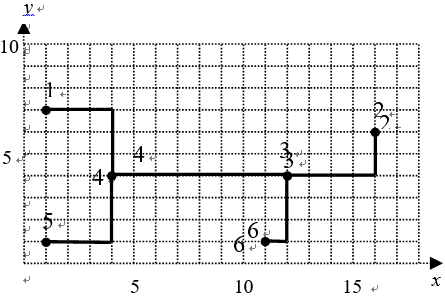
\includegraphics[width=0.5\textwidth]{bus.png}\\
SCORING\\
If your program outputs the correct answer for a test case within the time limit, then you get full points for that test case, and otherwise you get 0 points for that case.
\begin{lstlisting}[language=c++,breaklines=true] 
include <bits/stdc++.h>
using namespace std;

const int mxN=500;
int n, x[mxN], y[mxN], ans=1e9, nxt[mxN+1], d[mxN], e[mxN];
array<int, 2> a[mxN], mx[mxN+2][3], c[mxN][mxN];
vector<array<int, 2>> v;
bool b[mxN];

int main() {
    ifstream fin("bus.in");
    ofstream fout("bus.out");

    fin >> n;
    for(int i=0; i<n; ++i)
        fin >> x[i] >> y[i];
    for(int i=0; i<n; ++i) {
        for(int j=0; j<n; ++j)
            c[i][j]={abs(x[i]-x[j])+abs(y[i]-y[j]), j};
        sort(c[i], c[i]+n);
    }
    for(int i=0; i<n; ++i) {
        for(int j=0, k=0; j<n; j=k)
            for(; k<n&&c[i][k][0]==c[i][j][0]; ++k)
                d[c[i][k][1]]=j;
        for(int j=i+1; j<n; ++j) {
            iota(e, e+n, 0);
            for(int k=0; k<n; ++k)
		a[e[d[c[j][k][1]]]++]={abs(x[i]-x[c[j][k][1]])+abs(y[i]-y[c[j][k][1]]), c[j][k][0]};
            for(int l=0; l<3; ++l) {
                array<int, 2> c{};
                for(int k=n-1; ~k; --k) {
                    if(!b[k]&&a[k][1]>c[1]) {
                        c=a[k];
                        b[k]=1;
                    }
                }
            }
            v.push_back({});
            for(int k=0; k<n; ++k)
                if(b[k])
                    v.push_back(a[k]);
            memset(b, 0, n);
            memset(mx[v.size()], 0, 24);
            for(int k=v.size()-1; ~k; --k) {
                array<int, 2> c{v[k][1], k};
                memcpy(mx[k], mx[k+1], 24);
                for(int l=0; l<3; ++l)
                    if(mx[k][l]<c)
                        swap(mx[k][l], c);
            }
            for(int k=v.size()-1; ~k; --k)
                for(nxt[k]=k+1; nxt[k]<v.size()&&v[nxt[k]][1]<v[k][1]; nxt[k]=nxt[nxt[k]]);
            for(int k=0, dab=abs(x[i]-x[j])+abs(y[i]-y[j]); k<v.size(); ++k) {
                for(int l=k+1; l<v.size(); l=nxt[l]) {
                    array<int, 2> b0=mx[k+1][0], b1=mx[k+1][1];
                    if(b0[1]==l)
                        swap(b0, b1);
                    if(b1[1]==l)
                        b1=mx[k+1][2];
                    ans=min(max({v[k][0]+v[l][0], b0[0]+b1[0], v[l][0]+dab+b0[0]}), ans);
                }
            }
            v.clear();
        }
    }
    fout << ans;
}
\end{lstlisting}

\chapter{binary search}
\section{binarySearch}
 进击的奶牛
 题目描述
Farmer John 建造了一个有 $N$($2 \leq N \leq 10 ^ 5$) 个隔间的牛棚,这些隔间分布在一条直线上,坐标是 $x _ 1, x _ 2, \cdots, x _ N$($0 \leq x _ i \leq 10 ^ 9$)。
他的 $C$($2 \leq C \leq N$)头牛不满于隔间的位置分布,它们为牛棚里其他的牛的存在而愤怒。为了防止牛之间的互相打斗,Farmer John 想把这些牛安置在指定的隔间,所有牛中相邻两头的最近距离越大越好。那么,这个最大的最近距离是多少呢?
 输入格式
第 $1$ 行:两个用空格隔开的数字 $N$ 和 $C$。
第 $2 \sim N+1$ 行:每行一个整数,表示每个隔间的坐标。
 输出格式
输出只有一行,即相邻两头牛最大的最近距离。
 样例 1
 样例输入 1
5 3
1
2
8
4
9
 样例输出 1
3
\begin{lstlisting}[language=c++,breaklines=true]
include <iostream>
include <algorithm>
include <vector>

using namespace std;

bool check(vector<int>& stalls, int C, int dist) {
    int prev = stalls[0];
    int placed = 1;
    for (int i = 1; i < stalls.size(); ++i) {
        if (stalls[i] - prev >= dist) {
            prev = stalls[i];
            placed++;
            if (placed == C) return true;
        }
    }
    return false;
}

int binarySearch(vector<int>& stalls, int N, int C) {
    int left = 0;
    int right = stalls[N - 1] - stalls[0];
    int ans = 0;
    while (left <= right) {
        int mid = left + (right - left) / 2;
        if (check(stalls, C, mid)) {
            ans = mid;
            left = mid + 1;
        } else {
            right = mid - 1;
        }
    }
    return ans;
}

int main() {
    int N, C;
    cin >> N >> C;
    vector<int> stalls(N);
    for (int i = 0; i < N; ++i) {
        cin >> stalls[i];
    }
    sort(stalls.begin(), stalls.end());
    cout << binarySearch(stalls, N, C) << endl;
    return 0;
}
\end{lstlisting}

\section{}
 [NOIP2015 提高组] 跳石头
 题目背景
NOIP2015 Day2T1
 题目描述
一年一度的“跳石头”比赛又要开始了!
这项比赛将在一条笔直的河道中进行,河道中分布着一些巨大岩石。组委会已经选择好了两块岩石作为比赛起点和终点。在起点和终点之间,有 $N$ 块岩石(不含起点和终点的岩石)。在比赛过程中,选手们将从起点出发,每一步跳向相邻的岩石,直至到达终点。
为了提高比赛难度,组委会计划移走一些岩石,使得选手们在比赛过程中的最短跳跃距离尽可能长。由于预算限制,组委会至多从起点和终点之间移走 $M$ 块岩石(不能移走起点和终点的岩石)。
 输入格式
第一行包含三个整数 $L,N,M$,分别表示起点到终点的距离,起点和终点之间的岩石数,以及组委会至多移走的岩石数。保证 $L \geq 1$ 且 $N \geq M \geq 0$。
接下来 $N$ 行,每行一个整数,第 $i$ 行的整数 $D_i\,( 0 < D_i < L)$, 表示第 $i$ 块岩石与起点的距离。这些岩石按与起点距离从小到大的顺序给出,且不会有两个岩石出现在同一个位置。
 输出格式
一个整数,即最短跳跃距离的最大值。
 样例 1
 样例输入 1
25 5 2 
2
11
14
17 
21
 样例输出 1
4
 输入输出样例 1 说明
将与起点距离为 $2$ 和 $14$ 的两个岩石移走后,最短的跳跃距离为 $4$(从与起点距离 $17$ 的岩石跳到距离 $21$ 的岩石,或者从距离 $21$ 的岩石跳到终点)。
 数据规模与约定
对于 $20\%$的数据,$0 \le M \le N \le 10$。    
对于 $50\%$ 的数据,$0 \le M \le N \le 100$。  
对于 $100\%$ 的数据,$0 \le M \le N \le 50000,1 \le L 
 \le 10^9$。
\begin{lstlisting}[language=c++,breaklines=true]
include <iostream>
include <algorithm>

using namespace std;

const int MAXN = 50005;
int D[MAXN];

bool check(int mid, int L, int N, int M) {
    int prev = 0;
    int removed = 0;
    for (int i = 0; i <= N; ++i) {
        if (D[i] - prev < mid) {
            removed++;
            if (removed > M) return false;
        } else {
            prev = D[i];
        }
    }
    return true;
}

int main() {
    int L, N, M;
    cin >> L >> N >> M;
    for (int i = 0; i < N; ++i) {
        cin >> D[i];
    }
    D[N] = L;
    int left = 1, right = L;
    while (left < right) {
        int mid = (left + right + 1) / 2;
        if (check(mid, L, N, M)) {
            left = mid;
        } else {
            right = mid - 1;
        }
    }
    cout << left << endl;
    return 0;
}
\end{lstlisting}

\section{}
 [NOIP2001 提高组T1] 一元三次方程求解
 题目描述
有形如:$a x^3 + b x^2 + c x + d = 0$  这样的一个一元三次方程。给出该方程中各项的系数($a,b,c,d$ 均为实数),并约定该方程存在三个不同实根(根的范围在 $-100$ 至 $100$ 之间),且根与根之差的绝对值 $\ge 1$。要求由小到大依次在同一行输出这三个实根(根与根之间留有空格),并精确到小数点后 $2$ 位。
提示:记方程 $f(x) = 0$,若存在 $2$ 个数 $x_1$ 和 $x_2$,且 $x_1 < x_2$,$f(x_1) \times f(x_2) < 0$,则在 $(x_1, x_2)$ 之间一定有一个根。
 输入格式
一行,$4$ 个实数 $a, b, c, d$。
 输出格式
一行,$3$ 个实根,从小到大输出,并精确到小数点后 $2$ 位。
 样例 1
 样例输入 1
1 -5 -4 20
 样例输出 1
-2.00 2.00 5.00
\begin{lstlisting}[language=c++,breaklines=true]
include <iostream>
include <iomanip>
include <cmath>

double equation(double x, double a, double b, double c, double d) {
    return a * x * x * x + b * x * x + c * x + d;
}

void solveEquation(double a, double b, double c, double d) {
    for (double i = -100; i <= 100; i += 0.01) {
        double f1 = equation(i, a, b, c, d);
        double f2 = equation(i + 0.01, a, b, c, d);
        if (f1 * f2 < 0) {
            double root = i;
            while (std::abs(equation(root, a, b, c, d)) > 1e-6) {
                root = (root + root + 0.01) / 2;
            }
            std::cout << std::fixed << std::setprecision(2) << root << " ";
        }
    }
    std::cout << std::endl;
}

int main() {
    double a, b, c, d;
    std::cin >> a >> b >> c >> d;
    solveEquation(a, b, c, d);
    return 0;
}
\end{lstlisting}

\section{}
 [NOIP1998 普及组] 幂次方
 题目描述
任何一个正整数都可以用 $2$ 的幂次方表示。例如 $137=2^7+2^3+2^0 $。
同时约定次方用括号来表示,即 $a^b$ 可表示为 $a(b)$。
由此可知,$137$ 可表示为 $2(7)+2(3)+2(0)$
进一步:
$7= 2^2+2+2^0$  ( $2^1$ 用 $2$ 表示),并且 $3=2+2^0$。
所以最后 $137$ 可表示为 $2(2(2)+2+2(0))+2(2+2(0))+2(0)$。
又如 $1315=2^{10} +2^8 +2^5 +2+1$
所以 $1315$ 最后可表示为 $2(2(2+2(0))+2)+2(2(2+2(0)))+2(2(2)+2(0))+2+2(0)$。
 输入格式
一行一个正整数 $n$。
 输出格式
符合约定的 $n$ 的 $0, 2$ 表示(在表示中不能有空格)。
 样例 1
 样例输入 1
1315
 样例输出 1
2(2(2+2(0))+2)+2(2(2+2(0)))+2(2(2)+2(0))+2+2(0)
 提示
【数据范围】
对于 $100\%$ 的数据,$1 \le n \le 2 \times {10}^4$。
NOIP1998 普及组 第三题
\begin{lstlisting}[language=c++,breaklines=true]
include <iostream>
using namespace std;

void convert(int n) {
    if (n == 0) return;
    int power = 0;
    while ((1 << power) <= n) power++;
    power--;
    if (power > 1) {
        cout << "2(";
        convert(power);
        cout << ")";
    } else if (power == 1) {
        cout << "2";
    } else if (power == 0) {
        cout << "2(0)";
    }
    if (n - (1 << power)) {
        cout << "+";
        convert(n - (1 << power));
    }
}

int main() {
    int n;
    cin >> n;
    convert(n);
    cout << endl;
    return 0;
}
\end{lstlisting}

\section{}
\begin{lstlisting}[language=c++,breaklines=true]

\end{lstlisting}

\section{decode}
decode-csp-j-2022-2\\
【题目描述】\\
给定一个正整数$k$,有$k$次询问,每次给定三个正整数$n_i, e_i, d_i$求两个正整数$p_i
, q_i$,使$n_i = p_i \times q_i, e_i \times d_i = (p_i − 1)(q_i − 1) + 1$。\\
【输入格式】\\
从文件decode.in中读入数据。\\
第一行一个正整数$k$,表示有$k$次询问。\\
接下来$k$行,第$i$行三个正整数 $n_i, d_i, e_i$。\\
【输出格式】\\
输出到文件 decode.out 中。\\
输出$k$行,每行两个正整数$pi,qi$\\表示答案。\\
为使输出统一,你应当保证 $pi \leq qi$。\\
如果无解,请输出 NO。\\
【样例 1 输入】\\
\begin{tabular}{|c|c|c|}
  \hline
  1 & 10 \\
  2 & 770 77 5 \\
  3 & 633 1 211 \\
  4 & 545 1 499 \\
  5 & 683 3 227\\
  6 & 858 3 257\\
  7 & 723 37 13\\
  8 & 572 26 11\\
  9 & 867 17 17\\
  10 & 829 3 263\\
  11 & 528 4 109\\
  \hline
\end{tabular}\\
【样例 1 输出】\\
\begin{tabular}{|c|c|c|}
  \hline
  1 & 2 385 \\
  2 & NO \\
  3 & NO \\
  4 & NO \\
  5 & 11 78\\
  6 & 3 241\\
  7 & 2 286\\
  8 & NO\\
  9 & NO\\
  10 & 6 88\\
  \hline
\end{tabular}\\
【样例 2】\\
见选手目录下的 decode/decode2.in 与 decode/decode2.ans。\\
【样例 3】\\
见选手目录下的 decode/decode3.in 与 decode/decode3.ans。\\
【样例 4】\\
见选手目录下的 decode/decode4.in 与 decode/decode4.ans。\\
【数据范围】\\
以下记 $m = n − e \times d + 2$。\\
保证对于 $100\%$ 的数据,$1 \leq k \leq 10^5$,对于任意的 $1 \leq i \leq k,1 \leq n_i \leq 10^{18}
, 1 \leq ei \times di \leq 10^{18}, 1 \leq m \leq 10^9$。\\
\begin{tabular}{|c|c|c|c|c|}
  \hline
  测试点编号 & k $\leq$ & n $\leq$ & m $\leq$ & 特殊性质 \\
  \hline
  1 & & & & 保证有解\\
  \cline{1-1}
  \cline{5-1}
  2 & & $10^3$ & $10^3$ & 无\\
  \cline{1-1}
  \cline{3-1}
  \cline{4-1}
  \cline{5-1}
  3 & & & & 保证有解\\
  \cline{1-1}
  \cline{5-1}
  4 &  $10^3$ & $10^9$ & $6\times 10^4$ & 无\\
  \cline{1-1}
  \cline{4-1}
  \cline{5-1}
  5 & & & & 保证有解\\
  \cline{1-1}
  \cline{5-1}
  6 & & & & 无\\
  \cline{1-1}
  \cline{2-1}
  \cline{3-1}
  \cline{5-1}
  7 & & & & 保证若有解则 p = q\\
  \cline{1-1}
  \cline{5-1}
  8 & & & $10^{9}$ & 保证有解\\
  \cline{1-1}
   \cline{5-1}
  9 & $10^5$ & $10^{18}$ &  & \\
  \cline{1-1}
  10 & & & & 无\\
  \hline
\end{tabular}\\
解:\\
\begin{tabular}{|c|c|c|}
\hline
1 & input $n_i, e_i, d_i$ & 770 77 5\\
\hline
2 & output $pi,qi$ & 2 385\\
\hline
3 & $n_i = p_i \times q_i$ & $770 = 2\times 385$\\
\hline
4 & $e_i \times d_i = (p_i − 1)(q_i − 1) + 1$ & $77\times 5 = (2-1)\times(385 - 1) +1$\\
\hline
\end{tabular}\\
$\because
e_i \times d_i = (p_i − 1)(q_i − 1) + 1\\
e_id_i = p_iq_i - (p_i + q_i) + 2$\\
$\therefore
p_i + q_i = p_iq_i - e_id_i + 2$\\
令$s = p_i + q_i$\\
则有$s = p_iq_i - e_id_i + 2$\\
$s=n-d*e+2$
\begin{lstlisting}[language=C++]
include <iostream>
include <fstream>

using namespace std;

int main(){
	ifstream fin("decode.in");
	ofstream fout("decode.out");
	int k;
	fin>>k;
	for(int i = 0;i < k;i++){
		long long n,d,e;
		fin>>n>>d>>e;
		long long s = n - d * e + 2;
		long long left = 1,right = s - 1;
		long long p = -1, q = -1;

		while(left <= right){
			long long mid  = left + (right - left) / 2;
			if(mid * (s - mid) == n){
				p = mid;
				q = s - mid;	
				break;
			}else if(mid*(s-mid)<n){
				left = mid + 1;
			}else{
				right = mid - 1;
			}
		}
		if(p != -1 && q != -1 && p <= q){
			fout<<p<<" "<<q<<endl;
		}else{
			fout<<"NO"<<endl;
		}
	}
	fin.close();
	fout.close();
	return 0;
}
\end{lstlisting}

\chapter{prime}
\section{prime}
 [NOIP2012 普及组] 质因数分解
 题目描述
已知正整数 $n$ 是两个不同的质数的乘积,试求出两者中较大的那个质数。
 输入格式
输入一个正整数 $n$。
 输出格式
输出一个正整数 $p$,即较大的那个质数。
 样例 1
 样例输入 1
21
 样例输出 1
7
 提示
$1 \le n\le 2\times 10^9$
NOIP 2012 普及组 第一题
\begin{lstlisting}[language=c++,breaklines=true]
include <iostream>

using namespace std;

int main(){
	int n;
	cin>>n;
	for(int i = 2; i < n; i++){
		if(n % i == 0){
			cout<<max(i,n/i)<<endl;
			break;
		}
	}
	return 0;
}

\end{lstlisting}

\section{prime}
 [USACO1.5] 回文质数 Prime Palindromes\\
 题目描述\\
因为 $151$ 既是一个质数又是一个回文数(从左到右和从右到左是看一样的),所以 $151$ 是回文质数。\\
写一个程序来找出范围 $[a,b] (5 \le a < b \le 100,000,000)$(一亿)间的所有回文质数。\\
 输入格式\\
第一行输入两个正整数 $a$ 和 $b$。\\
 输出格式\\
输出一个回文质数的列表,一行一个。\\
 样例 1\\
 样例输入 1\\
5 500\\
 样例输出 1\\
5\\
7\\
11\\
101\\
131\\
151\\
181\\
191\\
313\\
353\\
373\\
383\\
 提示\\
Hint 1: Generate the palindromes and see if they are prime.\\
提示 1: 找出所有的回文数再判断它们是不是质数(素数).\\
Hint 2: Generate palindromes by combining digits properly. You might need more than one of the loops like below.\\
提示 2: 要产生正确的回文数,你可能需要几个像下面这样的循环。\\
产生长度为 $5$ 的回文数:\\
\begin{lstlisting}[language=C++,breaklines=true]
for (d1 = 1; d1 <= 9; d1+=2) {    // 只有奇数才会是素数
     for (d2 = 0; d2 <= 9; d2++) {
         for (d3 = 0; d3 <= 9; d3++) {
           palindrome = 10000*d1 + 1000*d2 +100*d3 + 10*d2 + d1;//(处理回文数...)
         }
     }
 }
\end{lstlisting}

\begin{lstlisting}[language=C++,breaklines=true]
include <iostream>
include <cmath>

bool isPrime(int n) {
    if (n < 2) return false;
    if (n == 2 || n == 3) return true;
    if (n % 2 == 0 || n % 3 == 0) return false;
    int sqrtN = sqrt(n);
    for (int i = 5; i <= sqrtN; i += 6) {
        if (n % i == 0 || n % (i + 2) == 0) return false;
    }
    return true;
}

bool isPalindrome(int n) {
    int original = n;
    int reversed = 0;
    while (n > 0) {
        reversed = reversed * 10 + n % 10;
        n /= 10;
    }
    return original == reversed;
}

int main() {
    int a, b;
    std::cin >> a >> b;
    for (int len = 1; ; ++len) {
        if (len % 2 == 0) {
            for (int firstHalf = pow(10, len / 2 - 1); firstHalf < pow(10, len / 2); ++firstHalf) {
                int palindrome = firstHalf;
                int temp = firstHalf;
                while (temp > 0) {
                    palindrome = palindrome * 10 + temp % 10;
                    temp /= 10;
                }
                if (palindrome >= a && palindrome <= b && isPrime(palindrome)) {
                    std::cout << palindrome << std::endl;
                }
            }
        } else {
            for (int firstHalf = pow(10, len / 2); firstHalf < pow(10, len / 2 + 1); ++firstHalf) {
                int palindrome = firstHalf;
                int temp = firstHalf / 10;
                while (temp > 0) {
                    palindrome = palindrome * 10 + temp % 10;
                    temp /= 10;
                }
                if (palindrome >= a && palindrome <= b && isPrime(palindrome)) {
                    std::cout << palindrome << std::endl;
                }
            }
        }
        if (len > 8) break;
    }
    return 0;
}
\end{lstlisting}

\section{prime}
 [NOIP2002 普及组] 选数
 题目描述
已知 $n$ 个整数 $x_1,x_2,\cdots,x_n$,以及 $1$ 个整数 $k$($k<n$)。从 $n$ 个整数中任选 $k$ 个整数相加,可分别得到一系列的和。例如当 $n=4$,$k=3$,$4$ 个整数分别为 $3,7,12,19$ 时,可得全部的组合与它们的和为:
$3+7+12=22$
$3+7+19=29$
$7+12+19=38$
$3+12+19=34$
现在,要求你计算出和为素数共有多少种。
例如上例,只有一种的和为素数:$3+7+19=29$。
 输入格式
第一行两个空格隔开的整数 $n,k$($1 \le n \le 20$,$k<n$)。
第二行 $n$ 个整数,分别为 $x_1,x_2,\cdots,x_n$($1 \le x_i \le 5\times 10^6$)。
 输出格式
输出一个整数,表示种类数。
 样例 1
 样例输入 1
4 3
3 7 12 19
 样例输出 1
1
 提示
【题目来源】
NOIP 2002 普及组第二题
\begin{lstlisting}[language=c++,breaklines=true]
include <iostream>
include <vector>
using namespace std;

bool isPrime(int num) {
    if (num < 2) return false;
    if (num == 2 || num == 3) return true;
    if (num % 2 == 0 || num % 3 == 0) return false;
    int i = 5;
    while (i * i <= num) {
        if (num % i == 0 || num % (i + 2) == 0) return false;
        i += 6;
    }
    return true;
}

int combinationSum(vector<int>& nums, int n, int k, int start, int sum, int count) {
    if (k == 0) {
        if (isPrime(sum)) return count + 1;
        else return count;
    }
    for (int i = start; i < n; i++) {
        count = combinationSum(nums, n, k - 1, i + 1, sum + nums[i], count);
    }
    return count;
}

int main() {
    int n, k;
    cin >> n >> k;
    vector<int> nums(n);
    for (int i = 0; i < n; i++) {
        cin >> nums[i];
    }
    int result = combinationSum(nums, n, k, 0, 0, 0);
    cout << result << endl;
    return 0;
}
\end{lstlisting}

\chapter{pq}
priority\_queue
\section{NOIP2004 提高组}
 [NOIP2004 提高组] 合并果子 / [USACO06NOV] Fence Repair G
 题目描述
在一个果园里,多多已经将所有的果子打了下来,而且按果子的不同种类分成了不同的堆。多多决定把所有的果子合成一堆。
每一次合并,多多可以把两堆果子合并到一起,消耗的体力等于两堆果子的重量之和。可以看出,所有的果子经过 $n-1$ 次合并之后, 就只剩下一堆了。多多在合并果子时总共消耗的体力等于每次合并所耗体力之和。
因为还要花大力气把这些果子搬回家,所以多多在合并果子时要尽可能地节省体力。假定每个果子重量都为 $1$ ,并且已知果子的种类 数和每种果子的数目,你的任务是设计出合并的次序方案,使多多耗费的体力最少,并输出这个最小的体力耗费值。
例如有 $3$ 种果子,数目依次为 $1$ , $2$ , $9$ 。可以先将 $1$ 、 $2$ 堆合并,新堆数目为 $3$ ,耗费体力为 $3$ 。接着,将新堆与原先的第三堆合并,又得到新的堆,数目为 $12$ ,耗费体力为 $12$ 。所以多多总共耗费体力 $=3+12=15$ 。可以证明 $15$ 为最小的体力耗费值。
 输入格式
共两行。  
第一行是一个整数 $n(1\leq n\leq 10000)$ ,表示果子的种类数。  
第二行包含 $n$ 个整数,用空格分隔,第 $i$ 个整数 $a_i(1\leq a_i\leq 20000)$ 是第 $i$ 种果子的数目。
 输出格式
一个整数,也就是最小的体力耗费值。输入数据保证这个值小于 $2^{31}$ 。
 样例 1
 样例输入 1
3 
1 2 9
 样例输出 1
15
 提示
对于 $30\%$ 的数据,保证有 $n \le 1000$:
对于 $50\%$ 的数据,保证有 $n \le 5000$;
对于全部的数据,保证有 $n \le 10000$。
\begin{lstlisting}[language=c++,breaklines=true]
include <iostream>
include <queue>

using namespace std;

int main() {
    int n;
    cin >> n;
    priority_queue<int, vector<int>, greater<int>> pq;
    for (int i = 0; i < n; i++) {
        int num;
        cin >> num;
        pq.push(num);
    }
    int ans = 0;
    while (pq.size() > 1) {
        int a = pq.top();
        pq.pop();
        int b = pq.top();
        pq.pop();
        ans += a + b;
        pq.push(a + b);
    }
    cout << ans << endl;
    return 0;
}
\end{lstlisting}

\chapter{greeedy}
\section{greedy}
 [USACO1.3] 混合牛奶 Mixing Milk
 题目描述
由于乳制品产业利润很低,所以降低原材料(牛奶)价格就变得十分重要。帮助 Marry 乳业找到最优的牛奶采购方案。
Marry 乳业从一些奶农手中采购牛奶,并且每一位奶农为乳制品加工企业提供的价格可能相同。此外,就像每头奶牛每天只能挤出固定数量的奶,每位奶农每天能提供的牛奶数量是一定的。每天 Marry 乳业可以从奶农手中采购到小于或者等于奶农最大产量的整数数量的牛奶。
给出 Marry 乳业每天对牛奶的需求量,还有每位奶农提供的牛奶单价和产量。计算采购足够数量的牛奶所需的最小花费。
注:每天所有奶农的总产量大于 Marry 乳业的需求量。
 输入格式
第一行二个整数 $n,m$,表示需要牛奶的总量,和提供牛奶的农民个数。
接下来 $m$ 行,每行两个整数 $p_i,a_i$,表示第 $i$ 个农民牛奶的单价,和农民 $i$ 一天最多能卖出的牛奶量。
 输出格式
单独的一行包含单独的一个整数,表示 Marry 的牛奶制造公司拿到所需的牛奶所要的最小费用。
 样例 1
 样例输入 1
100 5
5 20
9 40
3 10
8 80
6 30
 样例输出 1
630
 提示
【数据范围】  
对于 $100\%$ 的数据:  
$0 \le n,a_i \le 2 \times 10^6$,$0\le m \le 5000$,$0 \le p_i \le 1000$
题目翻译来自 NOCOW。
USACO Training Section 1.3
\begin{lstlisting}[language=c++,breaklines=true]
include <iostream>
include <algorithm>
include <vector>

using namespace std;

struct Farmer {
    int price;
    int amount;
};

bool compareFarmers(const Farmer& a, const Farmer& b) {
    return a.price < b.price;
}

int main() {
    int n, m;
    cin >> n >> m;
    vector<Farmer> farmers(m);
    for (int i = 0; i < m; ++i) {
        cin >> farmers[i].price >> farmers[i].amount;
    }
    sort(farmers.begin(), farmers.end(), compareFarmers);
    int total = 0;
    int cost = 0;
    for (int i = 0; i < m; ++i) {
        if (total + farmers[i].amount <= n) {
            total += farmers[i].amount;
            cost += farmers[i].price * farmers[i].amount;
        } else {
            int remaining = n - total;
            cost += farmers[i].price * remaining;
            break;
        }
    }
    cout << cost << endl;
    return 0;
}
\end{lstlisting}

\section{bookshelf}
 [USACO07DEC] Bookshelf B
 题目描述
Farmer John 最近为奶牛们的图书馆添置了一个巨大的书架,尽管它是如此的大,但它还是几乎瞬间就被各种各样的书塞满了。现在,只有书架的顶上还留有一点空间。 
所有 $N(1 \le N \le 20,000)$ 头奶牛都有一个确定的身高 $H_i(1 \le H_i \le 10,000)$。设所有奶牛身高的和为S。书架的高度为 $B$,并且保证 $1 \le B \le S < 2,000,000,007$。 
为了够到比最高的那头奶牛还要高的书架顶,奶牛们不得不像演杂技一般,一头站在另一头的背上,叠成一座“奶牛塔”。当然,这个塔的高度,就是塔中所有奶牛的身高之和。为了往书架顶上放东西,所有奶牛的身高和必须不小于书架的高度。
显然,塔中的奶牛数目越多,整座塔就越不稳定,于是奶牛们希望在能够到书架顶的前提下,让塔中奶牛的数目尽量少。 现在,奶牛们找到了你,希望你帮她们计算这个最小的数目。
 输入格式
* 第 $1$ 行: 2 个用空格隔开的整数:$N$ 和 $B$;
* 第 $4\dots N+1$ 行: 第 $i+1$ 行是 $1$ 个整数:$H_i$。
 输出格式
* 第 $1$ 行: 输出 $1$ 个整数,即最少要多少头奶牛叠成塔,才能够到书架顶部
 样例 1
 样例输入 1
6 40
6
18
11
13
19
11
 样例输出 1
3
 提示
输入说明:
一共有 $6$ 头奶牛,书架的高度为 $40$,奶牛们的身高在 $6\dots19$之间。
输出说明:
一种只用 $3$ 头奶牛就达到高度 $40$ 的方法:$18+11+13$。当然还有其他方法,在此不一一列出了。
\begin{lstlisting}[language=c++,breaklines=true]
include <iostream>
include <vector>
include <algorithm>

using namespace std;

int main() {
    int N, B;
    cin >> N >> B;
    
    vector<int> heights(N);
    
    // 输入奶牛身高
    for (int i = 0; i < N; ++i) {
        cin >> heights[i];
    }
    
    // 对奶牛身高进行降序排序
    sort(heights.begin(), heights.end(), greater<int>());
    
    int sum = 0;
    int count = 0;
    
    // 贪心累加身高,直到累加的高度大于等于书架高度B
    for (int i = 0; i < N; ++i) {
        sum += heights[i];
        count++;
        if (sum >= B) {
            break;
        }
    }
    
    // 输出最少的奶牛数目
    cout << count << endl;
    
    return 0;
}
\end{lstlisting}

\chapter{sort}
\section{alice}
 [CSP-J2019 江西] 次大值

 题目描述

Alice 有 $n$ 个正整数,数字从 $1 \sim n$ 编号,分别为 $a_1,a_2, \dots , a_n$。  
Bob 刚学习取模运算,于是便拿这 $n$ 个数进行练习,他写下了所有 

$$a_i \bmod a_j (1 \le i,j \le n \wedge i \neq j)$$  

的值,其中 $\bmod$ 表示取模运算。  

Alice 想知道所有的结果中,严格次大值是多少。将取模后得到的所有值进行去重,即相同的结果数值只保留一个,剩余数中第二大的值就称为严格次大值。

 输入格式

第一行一个正整数 $n$,表示数字个数。  
第二行 $n$ 个正整数表示 $a_i$。

 输出格式

仅一行一个整数表示答案。  
若取模结果去重后剩余数字不足两个,则输出 $-1$。

 样例 1

 样例输入 1

```
4
4 5 5 6
```

 样例输出 1

```
4
```

 样例 2

 样例输入 2

```
4
1 1 1 1
```

 样例输出 2

```
-1
```

 样例 3

 样例输入 3

```
7
12 3 8 5 7 20 15
```

 样例输出 3

```
12
```

 提示

【数据范围】  
对于 $40\%$ 的数据,$1\le n,a_i \le 100$;  
对于 $70\%$ 的数据,$1\le n \le 3000$,$1\le a_i \le 10^5$;  
对于 $100\%$ 的数据,$3 \le n \le 2\times 10^5$,$1\le a_i \le 10^9$。

【样例 $1$ 解释】  
所有取模的结果为 $\{4,4,4,1,0,5,1,0,5,2,1,1\}$。  
去重后有:$\{0,1,2,4,5 \}$,结果为 $4$。
\begin{lstlisting}[language=C++,breaklines=true]
include <cstdio>
include <iostream>
include <algorithm>
include <cstring>
using namespace std;
typedef long long LL;

int n;
int a[300005];

int main() {
    cin >> n;
    for(int i = 1; i <= n; i++)
        cin >> a[i];
    
    sort(a + 1, a + 1 + n); 
    n = unique(a + 1, a + 1 + n) - a - 1; // sort and remove duplicates
    
    if(n <= 1)
        printf("-1\n");
    else
        printf("%d\n", max(a[n - 2], a[n] % a[n - 1]));
    
    return 0;
}

\end{lstlisting}
\section{}
 [CSP-J 2021] 插入排序

 题目描述

插入排序是一种非常常见且简单的排序算法。小 Z 是一名大一的新生,今天 H 老师刚刚在上课的时候讲了插入排序算法。

假设比较两个元素的时间为 $\mathcal O(1)$,则插入排序可以以 $\mathcal O(n^2)$ 的时间复杂度完成长度为 $n$ 的数组的排序。不妨假设这 $n$ 个数字分别存储在 $a_1, a_2, \ldots, a_n$ 之中,则如下伪代码给出了插入排序算法的一种最简单的实现方式:

这下面是 C/C++ 的示范代码:

```cpp
for (int i = 1; i <= n; i++)
	for (int j = i; j >= 2; j--)
		if (a[j] < a[j-1]) {
			int t = a[j-1];
			a[j-1] = a[j];
			a[j] = t;
		}
```

这下面是 Pascal 的示范代码:

```pascal
for i:=1 to n do
	for j:=i downto 2 do
		if a[j]<a[j-1] then
			begin
				t:=a[i];
				a[i]:=a[j];
				a[j]:=t;
			end;
```

为了帮助小 Z 更好的理解插入排序,小 Z 的老师 H 老师留下了这么一道家庭作业:

H 老师给了一个长度为 $n$ 的数组 $a$,数组下标从 $1$ 开始,并且数组中的所有元素均为非负整数。小 Z 需要支持在数组 $a$ 上的 $Q$ 次操作,操作共两种,参数分别如下:

$1~x~v$:这是第一种操作,会将 $a$ 的第 $x$ 个元素,也就是 $a_x$ 的值,修改为 $v$。保证 $1 \le x \le n$,$1 \le v \le 10^9$。注意这种操作会改变数组的元素,修改得到的数组会被保留,也会影响后续的操作。

$2~x$:这是第二种操作,假设 H 老师按照上面的伪代码对 $a$ 数组进行排序,你需要告诉 H 老师原来 $a$ 的第 $x$ 个元素,也就是 $a_x$,在排序后的新数组所处的位置。保证 $1 \le x \le n$。注意这种操作不会改变数组的元素,排序后的数组不会被保留,也不会影响后续的操作。

H 老师不喜欢过多的修改,所以他保证类型 $1$ 的操作次数不超过 $5000$。

小 Z 没有学过计算机竞赛,因此小 Z 并不会做这道题。他找到了你来帮助他解决这个问题。

 输入格式

第一行,包含两个正整数 $n, Q$,表示数组长度和操作次数。

第二行,包含 $n$ 个空格分隔的非负整数,其中第 $i$ 个非负整数表示 $a_i$。

接下来 $Q$ 行,每行 $2 \sim 3$ 个正整数,表示一次操作,操作格式见【题目描述】。

 输出格式

对于每一次类型为 $2$ 的询问,输出一行一个正整数表示答案。

 样例 1

 样例输入 1

```
3 4
3 2 1
2 3
1 3 2
2 2
2 3
```

 样例输出 1

```
1
1
2
```

 提示

【样例解释 1】

在修改操作之前,假设 H 老师进行了一次插入排序,则原序列的三个元素在排序结束后所处的位置分别是 $3, 2, 1$。

在修改操作之后,假设 H 老师进行了一次插入排序,则原序列的三个元素在排序结束后所处的位置分别是 $3, 1, 2$。

注意虽然此时 $a_2 = a_3$,但是我们不能将其视为相同的元素。

【样例 2】

见附件中的 `sort/sort2.in` 与 `sort/sort2.ans`。

该测试点数据范围同测试点 $1 \sim 2$。

【样例 3】

见附件中的 `sort/sort3.in` 与 `sort/sort3.ans`。

该测试点数据范围同测试点 $3 \sim 7$。

【样例 4】

见附件中的 `sort/sort4.in` 与 `sort/sort4.ans`。

该测试点数据范围同测试点 $12 \sim 14$。

【数据范围】

对于所有测试数据,满足 $1 \le n \le 8000$,$1 \le Q \le 2 \times {10}^5$,$1 \le x \le n$,$1 \le v,a_i \le 10^9$。

对于所有测试数据,保证在所有 $Q$ 次操作中,至多有 $5000$ 次操作属于类型一。

各测试点的附加限制及分值如下表所示。

| 测试点 | $n \le$ | $Q \le$ | 特殊性质 |
|:-:|:-:|:-:|:-:|
| $1 \sim 4$ | $10$ | $10$ | 无 |
| $5 \sim 9$ | $300$ | $300$ | 无 |
| $10 \sim 13$ | $1500$ | $1500$ | 无 |
| $14 \sim 16$ | $8000$ | $8000$| 保证所有输入的 $a_i,v$ 互不相同 |
| $17 \sim 19$ | $8000$ | $8000$ | 无 |
| $20 \sim 22$ | $8000$ | $2 \times 10^5$ | 保证所有输入的 $a_i,v$ 互不相同 |
| $23 \sim 25$ | $8000$ | $2 \times 10^5$ | 无 |
\begin{lstlisting}[language=c++,breaklines=true]
include<iostream>
include<cstdio>
include<algorithm>
using namespace std;
const int MAXN=8005;
int n,q;
int t[MAXN];
struct node{
	int pre,id;
}a[MAXN];
bool cmp(node x,node y){
	if(x.pre!=y.pre) return x.pre<y.pre;
	return x.id<y.id;
}//两个元素之间的优先级
int main(){
	//freopen("sort.in","r",stdin);
	//freopen("sort.out","w",stdout);
	scanf("%d%d",&n,&q); 
	for(int i=1;i<=n;i++){
		scanf("%d",&a[i].pre);
		a[i].id=i;
	}//输入
	sort(a+1,a+n+1,cmp);//排序
	for(int i=1;i<=n;i++)
		t[a[i].id]=i;
	for(int i=1;i<=q;i++){
		int opt,x,v;
		scanf("%d",&opt);
		if(opt==1){//单点修改
			scanf("%d%d",&x,&v);//Ax->v
			a[t[x]].pre=v;
			for(int j=n;j>=2;j--)
				if(cmp(a[j],a[j-1])){
					node kkksc03=a[j];
					a[j]=a[j-1];
					a[j-1]=kkksc03;
				}//前扫
			for(int j=2;j<=n;j++)
				if(cmp(a[j],a[j-1])){
					node kkksc03=a[j];
					a[j]=a[j-1];
					a[j-1]=kkksc03;
				}//后扫
			for(int i=1;i<=n;i++)
				t[a[i].id]=i;//更新关系
		}
		else{
			scanf("%d",&x);
			printf("%d\n",t[x]);
		}
	}
	return 0;
}
\end{lstlisting}

\section{sort}
\begin{lstlisting}[language=c++]
include <iostream>
include <vector>
include <algorithm>

using namespace std;

int main(){
    std::vector<int> vec = {5, 2, 9, 1, 5, 6};
    std::sort(vec.begin(),vec.end(),std::greater<int>());
    for(int num:vec){
	    std::cout<<num<<"";
    }
}
\end{lstlisting}

\section{sort}
 [NOIP2009 普及组] 分数线划定
 题目描述
世博会志愿者的选拔工作正在 A 市如火如荼的进行。为了选拔最合适的人才,A 市对所有报名的选手进行了笔试,笔试分数达到面试分数线的选手方可进入面试。面试分数线根据计划录取人数的 $150\%$ 划定,即如果计划录取 $m$ 名志愿者,则面试分数线为排名第 $m \times 150\%$(向下取整)名的选手的分数,而最终进入面试的选手为笔试成绩不低于面试分数线的所有选手。
现在就请你编写程序划定面试分数线,并输出所有进入面试的选手的报名号和笔试成绩。
 输入格式
第一行,两个整数 $n,m(5 \leq n \leq 5000,3 \leq m \leq n)$,中间用一个空格隔开,其中 $n$ 表示报名参加笔试的选手总数,$m$ 表示计划录取的志愿者人数。输入数据保证 $m \times 150\%$ 向下取整后小于等于 $n$。
第二行到第 $n+1$ 行,每行包括两个整数,中间用一个空格隔开,分别是选手的报名号 $k(1000 \leq k \leq 9999)$和该选手的笔试成绩 $s(1 \leq s \leq 100)$。数据保证选手的报名号各不相同。
 输出格式
第一行,有 $2$ 个整数,用一个空格隔开,第一个整数表示面试分数线;第二个整数为进入面试的选手的实际人数。
从第二行开始,每行包含 $2$ 个整数,中间用一个空格隔开,分别表示进入面试的选手的报名号和笔试成绩,按照笔试成绩从高到低输出,如果成绩相同,则按报名号由小到大的顺序输出。
 样例 1
 样例输入 1
6 3 
1000 90 
3239 88 
2390 95 
7231 84 
1005 95 
1001 88
 样例输出 1
88 5 
1005 95 
2390 95 
1000 90 
1001 88 
3239 88
 提示
【样例说明】
$m \times 150\% = 3 \times150\% = 4.5$,向下取整后为 $4$。保证 $4$ 个人进入面试的分数线为 $88$,但因为 $88$ 有重分,所以所有成绩大于等于 $88$ 的选手都可以进入面试,故最终有 $5$ 个人进入面试。
NOIP 2009 普及组 第二题
\begin{lstlisting}[language=c++,breaklines=true]
    include <iostream>
    include <vector>
    include <algorithm>
    
    using namespace std;
    
    struct Applicant {
        int id;
        int score;
    };
    
    bool compare(const Applicant& a1, const Applicant& a2) {
        if (a1.score!= a2.score) {
            return a1.score > a2.score;
        } else {
            return a1.id < a2.id;
        }
    }
    
    int main() {
        int n, m;
        cin >> n >> m;
        vector<Applicant> applicants(n);
        for (int i = 0; i < n; i++) {
            cin >> applicants[i].id >> applicants[i].score;
        }
        sort(applicants.begin(), applicants.end(), compare);
        int interviewLine = applicants[m * 3 / 2 - 1].score;
        int count = 0;
        for (int i = 0; i < n; i++) {
            if (applicants[i].score >= interviewLine) {
                count++;
            }
        }
        cout << interviewLine << " " << count << endl;
        for (int i = 0; i < n; i++) {
            if (applicants[i].score >= interviewLine) {
                cout << applicants[i].id << " " << applicants[i].score << endl;
            }
        }
        return 0;
    }
\end{lstlisting}

\section{sort}
sort-csp-2021-2\\
【题目描述】\\
插入排序是一种非常常见且简单的排序算法。小$Z$是一名大一的新生,今天$H$老
师刚刚在上课的时候讲了插入排序算法。\\
假设比较两个元素的时间为$O(1)$,则插入排序可以以 $O(n^2)$ 的时间复杂度完成长
度为$n$的数组的排序。不妨假设这$n$个数字分别存储在$a_1, a_2, \cdots, a_n$之中,则如下伪
代码给出了插入排序算法的一种最简单的实现方式:\\
这下面是 C/C++ 的示范代码
\begin{lstlisting}[language=C++,breaklines=true]
for(int i = 1; i <= n; i++){
	for(int j = i; j >= 2; j--){
		if(a[j] < a[j - 1]){
			int t = a[j - 1];
			a[j - 1] = a[j];
			a[j] = t;
		}
	}
}
\end{lstlisting}
为了帮助小$Z$更好的理解插入排序,小$Z$的老师$H$老师留下了这么一道家庭作业:\\
$H$老师给了一个长度为$n$的数组$a$,数组下标从1开始,并且数组中的所有元素均
为非负整数。小$Z$需要支持在数组$a$上的$Q$次操作,操作共两种,参数分别如下:\\
$1\quad x\quad v$ : 这是第一种操作,会将$a$的第$x$个元素,也就是$a_x$的值,修改为$v$。保证
$1 \leq x \leq n$, $1 \leq v \leq 10^9$。
注意这种操作会改变数组的元素,修改得到的数组会被保留,也会影响后续的操作。\\
$2\quad x$ : 这是第二种操作,假设$H$老师按照上面的伪代码对$a$数组进行排序,你需要
告诉$H$老师原来$a$的第$x$个元素,也就是$a_x$,在排序后的新数组所处的位置。保证$1\leq x \leq n$。注意这种操作不会改变数组的元素,排序后的数组不会被保留,也不会影响后续的操作。\\
$H$老师不喜欢过多的修改,所以他保证类型1的操作次数不超过5000。\\
小$Z$没有学过计算机竞赛,因此小$Z$并不会做这道题。他找到了你来帮助他解决
这个问题。\\
【输入格式】\\
从文件sort.in中读入数据。\\
输入的第一行包含两个正整数 $n, q$,表示数组长度和操作次数。保证 $1 \leq n \leq
8, 000, 1 \leq q \leq 2 \times 10^5$。\\
输入的第二行包含$n$个空格分隔的非负整数,其中第$i$个非负整数表示$a_i$。保证
$1 \leq a_i \leq 10^9$。\\
接下来$q$行,每行$2 \sim 3$ 个正整数,表示一次操作,操作格式见题目描述。\\
【输出格式】\\
输出到文件sort.out中。\\
对于每一次类型为 2 的询问,输出一行一个正整数表示答案。\\
【样例 1 输入】\\
\begin{tabular}{|c|}
  \hline
  3 4 \\
  3 2 1 \\
  2 3 \\
  1 3 2 \\
  2 2 \\
  2 3 \\
  \hline
\end{tabular}\\
【样例 1 输出】\\
\begin{tabular}{|c|}
  \hline
  1 \\
  1 \\
  2 \\
  \hline
\end{tabular}\\
【样例 1 解释】\\
在修改操作之前,假设$H$老师进行了一次插入排序,则原序列的三个元素在排序
结束后所处的位置分别是 3, 2, 1。\\
在修改操作之前,假设$H$老师进行了一次插入排序,则原序列的三个元素在排序
结束后所处的位置分别是 3, 1, 2。\\
注意虽然此时 $a_2 = a_3$,但是我们不能将其视为相同的元素。\\
解:
\begin{lstlisting}[language=C++,breaklines=true]
include <iostream>
include <fstream>
include <algorithm>

using namespace std;

struct node {
    int id;
    int num;
};

node a[8010];
int b[8010];
int n, q;

void change(int pos) {
    while (pos > 1) {
        if (a[pos].num == a[pos - 1].num && a[pos].id > a[pos - 1].id) break;
        if (a[pos].num > a[pos - 1].num) break;
        swap(a[pos], a[pos - 1]);
        b[a[pos].id] = pos;
        pos--;
    }
    while (pos < n) {
        if (a[pos].num == a[pos + 1].num && a[pos].id < a[pos + 1].id) break;
        if (a[pos].num < a[pos + 1].num) break;
        swap(a[pos], a[pos + 1]);
        b[a[pos].id] = pos;
        pos++;
    }
}

bool cmp(node a, node b) {
    if (a.num == b.num) return a.id < b.id;
    else return a.num < b.num;
}

int main() {
    ifstream fin("sort.in");
    ofstream fout("sort.out");

    fin >> n >> q;
    for (int i = 1; i <= n; i++) {
        fin >> a[i].num;
        a[i].id = i;
    }

    sort(a + 1, a + 1 + n, cmp);
    for (int i = 1; i <= n; i++) {
        b[a[i].id] = i;
    }

    while (q--) {
        int op, x, v;
        fin >> op;
        if (op == 1) {
            fin >> x >> v;
            a[b[x]].num = v;
            change(b[x]);
            for (int i = 1; i <= n; i++) {
                b[a[i].id] = i;
            }
        } else {
            fin >> x;
            fout << b[x] << endl;
        }
    }

    fin.close();
    fout.close();
    return 0;
}
\end{lstlisting}


\section{NOIP2007 普及组 T1}
[NOIP2007 普及组] 奖学金
 题目背景
 题目描述
某小学最近得到了一笔赞助,打算拿出其中一部分为学习成绩优秀的前 $5$ 名学生发奖学金。期末,每个学生都有 $3$ 门课的成绩:语文、数学、英语。先按总分从高到低排序,如果两个同学总分相同,再按语文成绩从高到低排序,如果两个同学总分和语文成绩都相同,那么规定学号小的同学排在前面,这样,每个学生的排序是唯一确定的。
任务:先根据输入的 $3$ 门课的成绩计算总分,然后按上述规则排序,最后按排名顺序输出前五名名学生的学号和总分。
注意,在前 $5$ 名同学中,每个人的奖学金都不相同,因此,你必须严格按上述规则排序。例如,在某个正确答案中,如果前两行的输出数据(每行输出两个数:学号、总分) 是:
```plain
7 279  
5 279
这两行数据的含义是:总分最高的两个同学的学号依次是 $7$ 号、$5$ 号。这两名同学的总分都是 $279$ (总分等于输入的语文、数学、英语三科成绩之和) ,但学号为 $7$ 的学生语文成绩更高一些。
如果你的前两名的输出数据是:
```plain
5 279  
7 279
则按输出错误处理,不能得分。
 输入格式
共 $n+1$ 行。
第 $1$ 行为一个正整数 $n \le 300$,表示该校参加评选的学生人数。
第 $2$ 到 $n+1$ 行,每行有 $3$ 个用空格隔开的数字,每个数字都在 $0$ 到 $100$ 之间。第 $j$ 行的 $3$ 个数字依次表示学号为 $j-1$ 的学生的语文、数学、英语的成绩。每个学生的学号按照输入顺序编号为 $1\sim n$(恰好是输入数据的行号减 $1$)。
保证所给的数据都是正确的,不必检验。
 输出格式
共 $5$ 行,每行是两个用空格隔开的正整数,依次表示前 $5$ 名学生的学号和总分。
 样例 1
 样例输入 1
6
90 67 80
87 66 91
78 89 91
88 99 77
67 89 64
78 89 98
 样例输出 1
6 265
4 264
3 258
2 244
1 237
 样例 2
 样例输入 2
8
80 89 89
88 98 78
90 67 80
87 66 91
78 89 91
88 99 77
67 89 64
78 89 98
 样例输出 2
8 265
2 264
6 264
1 258
5 258
\begin{lstlisting}[language=c++,breaklines=true]
include <iostream>
include <algorithm>
include <vector>

using namespace std;

struct Student {
    int id;
    int chinese;
    int math;
    int english;
    int total;
};

bool compare(const Student& s1, const Student& s2) {
    if (s1.total!= s2.total) {
        return s1.total > s2.total;
    } else if (s1.chinese!= s2.chinese) {
        return s1.chinese > s2.chinese;
    } else {
        return s1.id < s2.id;
    }
}

int main() {
    int n;
    cin >> n;
    vector<Student> students(n);
    for (int i = 0; i < n; i++) {
        students[i].id = i + 1;
        cin >> students[i].chinese >> students[i].math >> students[i].english;
        students[i].total = students[i].chinese + students[i].math + students[i].english;
    }
    sort(students.begin(), students.end(), compare);
    for (int i = 0; i < 5; i++) {
        cout << students[i].id << " " << students[i].total << endl;
    }
    return 0;
}
\end{lstlisting}

\section{NOIP 2006 普及组 第一题}
 [NOIP2006 普及组] 明明的随机数\\
 题目描述\\
明明想在学校中请一些同学一起做一项问卷调查,为了实验的客观性,他先用计算机生成了 $N$ 个 $1$ 到 $1000$ 之间的随机整数 $(N\leq100)$,对于其中重复的数字,只保留一个,把其余相同的数去掉,不同的数对应着不同的学生的学号。然后再把这些数从小到大排序,按照排好的顺序去找同学做调查。请你协助明明完成“去重”与“排序”的工作。
 输入格式\\
输入有两行,第 $1$ 行为 $1$ 个正整数,表示所生成的随机数的个数 $N$。\\
第 $2$ 行有 $N$ 个用空格隔开的正整数,为所产生的随机数。\\
 输出格式\\
输出也是两行,第 $1$ 行为 $1$ 个正整数 $M$,表示不相同的随机数的个数。\\
第 $2$ 行为 $M$ 个用空格隔开的正整数,为从小到大排好序的不相同的随机数。\\
 样例 1\\
 样例输入 1\\
10\\
20 40 32 67 40 20 89 300 400 15\\
 样例输出 1\\
8\\
15 20 32 40 67 89 300 400\\
 提示\\
NOIP 2006 普及组 第一题\\
\begin{lstlisting}[language=c++]
include <iostream>
include <set>
include <vector>
include <algorithm>

using namespace std;

int main() {
    int N;
    // 输入随机数个数
    cin >> N;

    set<int> unique_numbers; // 用 set 自动去重
    for (int i = 0; i < N; ++i) {
        int num;
        cin >> num;
        unique_numbers.insert(num); // 插入 set,自动去重
    }

    // 将 set 中的元素复制到 vector 进行排序
    vector<int> sorted_numbers(unique_numbers.begin(), unique_numbers.end());
    sort(sorted_numbers.begin(), sorted_numbers.end()); // 排序

    // 输出去重后数字的个数
    cout << sorted_numbers.size() << endl;

    // 输出排序后的数字
    for (int num : sorted_numbers) {
        cout << num << " ";
    }
    cout << endl;

    return 0;
}
\end{lstlisting}

\section{NOIP1998 提高组}
 [NOIP1998 提高组] 拼数
 题目描述
设有 $n$ 个正整数 $a_1 \dots a_n$,将它们联接成一排,相邻数字首尾相接,组成一个最大的整数。
 输入格式
第一行有一个整数,表示数字个数 $n$。
第二行有 $n$ 个整数,表示给出的 $n$ 个整数 $a_i$。
 输出格式
一个正整数,表示最大的整数
 样例 1
 样例输入 1
3
13 312 343
 样例输出 1
34331213
 样例 2
 样例输入 2
4
7 13 4 246
 样例输出 2
7424613
 提示
对于全部的测试点,保证 $1 \leq n \leq 20$,$1 \leq a_i \leq 10^9$。
NOIP1998 提高组 第二题
\begin{lstlisting}[language=c++,breaklines=true]
include <iostream>
include <vector>
include <string>
include <algorithm>

using namespace std;

bool compare(const string& a, const string& b) {
    return a + b > b + a;
}

int main() {
    int n;
    cin >> n;
    vector<string> numbers(n);
    for (int i = 0; i < n; i++) {
        cin >> numbers[i];
    }
    sort(numbers.begin(), numbers.end(), compare);
    string result;
    for (const string& num : numbers) {
        result += num;
    }
    cout << result << endl;
    return 0;
}
\end{lstlisting}


\section{number}
number-csp-j-2019-1\\
【题目描述】\\
小$K$同学向小$P$同学发送了一个长度为8的01字符串来玩数字游戏,小$P$同学想要知道字符串中究竟有多少个1。\\
注意:01字符串为每一个字符是0或者1的字符串,如“101”(不含双引号)为一个长度为3的01字符串。\\
【输入格式】\\
输入文件名为number.in\\
输入文件只有一行,一个长度为8的01字符串$s$。\\
【输出格式】\\
输出文件名为number.out\\
输出文件只有一行,包含一个整数,即01字符串中字符1的个数。\\
【输入输出样例1】\\
\begin{tabular}{|c|c|}
\hline
number.in & number.out\\
\hline
00010100 & 2\\
\hline
\end{tabular}\\
【输入输出样例2】\\
\begin{tabular}{|c|c|}
\hline
number.in & number.out\\
\hline
11111111 & 8\\
\hline
\end{tabular}\\
解:\\
\begin{tabular}{|c|c|}
\hline
1 & s[i] == '1'\\
\hline
2 & count++; \\
\hline
\end{tabular}
\begin{lstlisting}[language=c++]
include <iostream>
include <fstream>
include <string>

using namespace std;

int main(){
	ifstream fin("number.in");
	ofstream fout("number.out");

	string s;
	fin>>s;
	int count = 0;

	for(int i = 0; i < s.length();i++){
		if(s[i] == '1'){
			count++;
		}
	}
	fout<<count;

	fin.close();
	fout.close();
	return 0;
}
\end{lstlisting}

\section{noip2018-1}
NOIP2018普及组T1标题统计\\
凯凯刚写了一篇美妙的作文,请问这篇作文的标题中有多少个字符? 注意:标题中可能包含大、小写英文字母、数字字符、空格和换行符。统计标题字符数时,空格和换行符不计算在内。\\
输入格式\\
输入文件只有一行,一个字符串 $s$。\\
输出格式\\
输出文件只有一行,包含一个整数,即作文标题的字符数(不含空格和换行符)。\\
样例 1\\
样例输入 1\\
234\\
样例输出 1\\
3\\
 样例 2\\
 样例输入 2\\
Ca 45\\
 样例输出 2\\
4\\
 提示\\
样例 1 说明   \\
标题中共有 3 个字符,这 3 个字符都是数字字符。\\
样例 2 说明\\
标题中共有 $ 5$ 个字符,包括 $1$ 个大写英文字母, $1$ 个小写英文字母和 $2$ 个数字字符, 还有 $1$ 个空格。由于空格不计入结果中,故标题的有效字符数为 $4$ 个。 
数据规模与约定\\
规定 $|s|$ 表示字符串 $s$ 的长度(即字符串中的字符和空格数)。\\    
对于 $40\%$ 的数据,$1 ≤ |s| ≤ 5$,保证输入为数字字符及行末换行符。\\   
对于 $80\%$ 的数据,$1 ≤ |s| ≤ 5$,输入只可能包含大、小写英文字母、数字字符及行末换行符。\\   
对于 $100\%$ 的数据,$1 ≤ |s| ≤ 5$,输入可能包含大、小写英文字母、数字字符、空格和行末换行符。\\
\begin{lstlisting}[language=C++,breaklines=true]
include <iostream>

using namespace std;

int main(){
	string s;
	getline(cin,s);
	int count = 0;
	for(char c : s){
		if(c != ' ' && c != '\n'){
			count++;
		}
	}
	cout<<count<<endl;
	return 0;
}
\end{lstlisting}

\section{noip2012-1}
 [NOIP2012 普及组] 质因数分解\\
 题目描述\\
已知正整数 $n$ 是两个不同的质数的乘积,试求出两者中较大的那个质数。\\
 输入格式\\
输入一个正整数 $n$。\\
 输出格式\\
输出一个正整数 $p$,即较大的那个质数。\\
 样例 1\\
 样例输入 1\\
21\\
 样例输出 1\\
7\\
 提示\\
$1 \le n\le 2\times 10^9$
\begin{lstlisting}[language=C++,breaklines=true]
include <iostream>

using namespace std;

int main(){
	int n;
	cin>>n;
	for(int i = 2; i < n; i++){
		if(n % i == 0){
			cout<<max(i,n/i)<<endl;
			break;
		}
	}
	return 0;
}
\end{lstlisting}

\chapter{mathematics}
\section{gcd}
Greatest Common Divisor最大公约数\\
辗转相除法(欧几里得算法)\\
原理:\\
两个整数的最大公约数等于其中较小的数和两数相除余数的最大公约数。\\
不断用较大数除以较小数取余数,直到余数为 0,此时较小数就是最大公约数。\\
代码模板:
\begin{lstlisting}[language=C++]
include <iostream>
using namespace std;

int gcd(int a,int b){
	int temp;
	while(b != 0){
		temp = a % b;
		a = b;
		b = temp;
	}
	return a;
}

int main(){
	cout<<"Please input two numbers:"<<endl;
	int a,b;
	cin>>a>>b;
	cout<<gcd(a,b)<<endl;
}
\end{lstlisting}

\section{pow}
pow-csp-j-2022-1\\
【题目描述】\\
小文同学刚刚接触了信息学竞赛,有一天她遇到了这样一个题:给定正整数a和b,求$a^b$的值是多少。\\
$a^b$即b个a相乘的值,例如$2^3$即为3个2相乘,结果为$2\times2\times2=8$。\\
“简单!”小文心想,同时很快就写出了一份程序,可是测试时却出现了错误。\\
小文很快意识到,她的程序里的变量都是 int 类型的。在大多数机器上,int 类型
能表示的最大数为$2^{31}−1$,因此只要计算结果超过这个数,她的程序就会出现错误。\\
由于小文刚刚学会编程,她担心使用 int 计算会出现问题。因此她希望你在 $a^b$ 的
值超过 $10^9$ 时,输出一个 ‐1 进行警示,否则就输出正确的 $a^b$ 的值。\\
然而小文还是不知道怎么实现这份程序,因此她想请你帮忙。\\
【输入格式】\\
从文件 $pow.in$ 中读入数据。\\
输入共一行,两个正整数 a, b 。\\
【输出格式】\\
输出到文件$pow.out$中。\\
输出共一行,如果 $a^b$ 的值不超过 $10^9$ ,则输出 $a^b$ 的值,否则输出 ‐1 。\\
【样例 1 输入】\\
10 9\\
【样例 1 输出】\\
1000000000\\
【样例 2 输入】\\
23333 66666\\
【样例 2 输出】\\
‐1\\
【数据范围】\\
对于 $10\%$ 的数据,保证 b = 1\\
对于 $30\%$ 的数据,保证 $b \leq 2$\\
对于 $60\%$ 的数据,保证 $b \leq 30, a^b \leq 10^{18}$\\
对于 $100\%$ 的数据,保证 $1 \leq a, b \leq 10^9$\\
解:\\
\begin{tabular}{|c|c|}
\hline
1 & result *= a;\\
\hline
\end{tabular}
\begin{lstlisting}[language=C++]
include <iostream>
include <fstream>

using namespace std;

int main(){
	ifstream fin("pow.in");
	ofstream fout("pow.out");

	int a,b;
	fin>>a>>b;
	long long result = 1;
	for(int i = 1; i <= b; i++){
		result *= a;
		if(result > 1e9){
			fout<<-1;
			return 0;
		}
	}
	fout<<result;
	return 0;
}
\end{lstlisting}

\section{power}
power-csp-j-2020\\
【题目描述】\\
一般来说,一个正整数可以拆分成若干个正整数的和。例如, $1 = 1, 10 =
1 + 2 + 3 + 4 $等。\\
对于正整数$n$的一种特定拆分,我们称它为“优秀的”,当且仅当在这种拆
分下$n$被分解为了若干个不同的2的正整数次幂。注意,一个数$x$能被表
示成2的正整数次幂,当且仅当$x$能通过正整数个2相乘在一起得到。\\
例如, $10 = 8 + 2 = 2^3 + 2^1$ 是一个优秀的拆分。但是, $7 = 4 + 2 + 1 =
2^2 + 2^1 + 2^0$ 就不是一个优秀的拆分,因为1不是2的正整数次幂。\\
现在,给定正整数$n$,你需要判断这个数的所有拆分中,是否存在优秀的
拆分。 若存在, 请你给出具体的拆分方案。\\
【输入格式】\\
输入文件名为 power.in。\\
输入文件只有一行,一个正整数$n$,代表需要判断的数。\\
【输出格式】\\
输出文件名为 power.out。\\
如果这个数的所有拆分中,存在优秀的拆分。那么, 你需要从大到小输出
这个拆分中的每一个数, 相邻两个数之间用一个空格隔开。 可以证明, 在规定
了拆分数字的顺序后, 该拆分方案是唯一的。\\
若不存在优秀的拆分,输出“-1”(不包含双引号)。\\
【样例 1 输入】\\
6\\
【样例 1 输出】\\
4 2\\
【样例 1 解释】\\
$6 = 4 + 2 = 2^2 + 2^1$ 是一个优秀的拆分。注意, 6 = 2 + 2 + 2 不是一个优
秀的拆分,因为拆分成的3个数不满足每个数互不相同。\\
【样例 2 输入】\\
7\\
【样例 2 输出】\\
-1\\
【样例 3】\\
见选手目录下的 power/power3.in 与 power/power3.ans。\\
【数据范围与提示】\\
对于 20\% 的数据,$n\leq 10$。\\
对于另外20\%的数据,保证$n$为奇数。\\
对于另外20\%的数据,保证$n$为2的正整数次幂。\\
对于 80\% 的数据, $n\leq 1024$。\\
对于 100\% 的数据, $1\leq n\leq 1\times10^7$。\\
解:\\
\begin{tabular}{|c|c|c|c|c|}
\hline
1 & input &6 & 7\\
\hline
2 & output & 4 2 & -1\\
\hline
3 & $2^1,2^2,...,2^n$ & $power = 1\ll i$& \\
\hline
\end{tabular}
\begin{lstlisting}[language=C++,breaklines=true]
include <iostream>
include <cmath>

const int maxn = 100005;

int main() {
    int n;
    std::cin >> n;

    if (n % 2!= 0) {
        std::cout << "-1" << std::endl;
        return 0;
    }

    long long now = 1;
    bool a[105] = {false};
    int i = 0;
    while (now * 2 <= n) {
        now *= 2;
        i++;
    }

    int i1 = i;
    while (now > 1) {
        if (n - now >= 0) {
            a[i1] = true;
            n -= now;
        }
        i1--;
        now /= 2;
    }

    for (int j = i; j >= 1; --j) {
        if (!a[j]) continue;
        long long ans = std::pow(2, j);
        std::cout << ans << " ";
    }

    return 0;
}
\end{lstlisting}

\section{area}
CSP-J2019江西 面积\\
题目描述\\
Alice 有一个边长为 $a$ 的正方形,Bob 有一个长宽分别为 $b,c$ 的矩形,请你告诉他们俩谁的图形面积更大。\\
输入格式\\
仅一行三个正整数 $a,b,c$\\
输出格式\\
输出仅一行一个字符串,若正方形面积大则输出 `Alice`,否则输出 `Bob`。\\
样例1\\
样例输入1\\
5 4 6\\
样例输出 1\\
Alice\\
样例 2\\
样例输入 2\\
7 5 10\\
样例输出 2\\
Bob\\
提示\\
【数据范围】\\   
对于 $30\%$ 的数据,$1 \le a,b,c \le 100$,$b=c$;\\  
对于 $80\%$ 的数据,$1\le a,b,c \le 10^4$;\\
对于 $100\%$ 的数据,$1\le a,b,c \le 10^9$。\\
【样例 $1$ 解释】\\  
正方形面积为  $25$,矩形面积为 $24$。\\
【样例 $2$ 解释】\\  
正方形面积为  $49$,矩形面积为 $50$。\\
\begin{lstlisting}[language=C++,breaklines=true]
include <iostream>
using namespace std;

int main() {
    long long a, b, c;
    cin >> a >> b >> c;
    if (a*a > b*c) {
        cout << "Alice";
    } else {
        cout << "Bob";
    }
    return 0;
}
\end{lstlisting}

\section{char}
字母转换\\
输入一个小写字母,输出其对应的大写字母。例如输入a,输出A。\\
样例\\
样例输入a\\
样例输出A
\begin{lstlisting}[language=C++,breaklines=true]
include <iostream>
using namespace std;
int main(){
    char ch,res;
    cin>>ch;
    res = ch - 'a' + 'A';
    cout<<res;
}
\end{lstlisting}

\section{numberReverse}
数字反转\\
输入一个不小于 $1000$ 且小于 $10000$,同时包括小数点后一位的一个浮点数,例如 $1234.5$ ,要求把这个数字翻转过来,变成 $5.4321$ 并输出。\\
输入格式\\
一行一个浮点数\\
输出格式\\
一行一个浮点数\\
样例\\
样例输入\\
1234.5\\
样例输出\\
5.4321\\
\begin{lstlisting}[language=C++,breaklines=true]

\end{lstlisting}

\section{buyPencil}
[NOIP2016 普及组] 买铅笔\\
P老师需要去商店买 $n$ 支铅笔作为小朋友们参加 NOIP 的礼物。她发现商店一共有 $3$ 种包装的铅笔,不同包装内的铅笔数量有可能不同,价格也有可能不同。为了公平起 见,P 老师决定只买同一种包装的铅笔。
商店不允许将铅笔的包装拆开,因此 P 老师可能需要购买超过 $n$ 支铅笔才够给小朋友们发礼物。
现在 P 老师想知道,在商店每种包装的数量都足够的情况下,要买够至少 $n$ 支铅笔最少需要花费多少钱。
 输入格式\\
第一行包含一个正整数 $n$,表示需要的铅笔数量。\\
接下来三行,每行用 $2$ 个正整数描述一种包装的铅笔:其中第 $1$ 个整数表示这种包装内铅笔的数量,第 $2$ 个整数表示这种包装的价格。
保证所有的 $7$ 个数都是不超过 $10000$ 的正整数。\\
 输出格式\\
$1$ 个整数,表示 P 老师最少需要花费的钱。\\
 样例 1\\
 样例输入 1\\
57\\
2 2\\
50 30\\
30 27\\
 样例输出 1\\
54\\
 样例 2\\
 样例输入 2\\
9998\\
128 233\\
128 2333\\
128 666\\
 样例输出 2\\
18407\\
 样例 3\\
 样例输入 3\\
9999\\
101 1111\\
1 9999\\
1111 9999\\
 样例输出 3\\
89991\\
 提示\\
铅笔的三种包装分别是:\\
- $2$ 支装,价格为 $2$;\\
- $50$ 支装,价格为 $30$;\\
- $30$ 支装,价格为 $27$。\\
P 老师需要购买至少 $57$ 支铅笔。\\
如果她选择购买第一种包装,那么她需要购买 $29$ 份,共计 $2 \times 29 = 58$ 支,需要花费的钱为 $2 \times 29 = 58$。
实际上,P 老师会选择购买第三种包装,这样需要买 $2$ 份。虽然最后买到的铅笔数量更多了,为 $30 \times 2 = 60$ 支,但花费却减少为 $27 \times 2 = 54$,比第一种少。
对于第二种包装,虽然每支铅笔的价格是最低的,但要够发必须买 $2$ 份,实际的花费达到了 $30  \times 2 = 60$,因此 P 老师也不会选择。
所以最后输出的答案是 $54$。\\
数据范围\\
保证所有的 $7$ 个数都是不超过 $10000$ 的正整数。\\
子任务\\
子任务会给出部分测试数据的特点。如果你在解决题目中遇到了困难,可以尝试只解决一部分测试数据。\\
每个测试点的数据规模及特点如下表:\\
上表中“整倍数”的意义为:若为 $K$,表示对应数据所需要的铅笔数量 $n$ —定是每种包装铅笔数量的整倍数(这意味着一定可以不用多买铅笔)。
\begin{lstlisting}[language=C++,breaklines=true]

\end{lstlisting}

\chapter{bipartite graph}
\section{transform}
NOI2009-1 transform变换序列\\
【问题描述】\\    
对于$N$个整数$0, 1,\cdots, N-1$,一个变换序列$T$可以将$i$变成$Ti$,其中$T_{i}\in\{0,1,\cdots,N-1\}$且$\bigcup_{i=0}^{N-1}{T_i}=\{0,1,\cdots,N-1\}$。$\forall x,y\in\{0,1,\cdots,N-1\}$定义$x$和$y$之间的距离$D(x,y) = min\{|x - y|, N - |x - y|\}$。给定每个$i$和$T_i$之间的距离$D(i,T_i)$,你需要求出一个满足要求的变换序列$T$。如果有多个满足条件的序列,输出其中字典序最小的一个。\\
说明:对于两个变换序列$S$和$T$,如果存在$p<N$,满足对于$i=0,1,\cdots p-1$,$S_i=T_i$且$S_p<T_p$,我们称$S$比$T$字典序小。\\
【输入文件】\\
输入文件$transform.in$的第一行包含一个整数$N$,表示序列的长度。接下来的一行包含$N$个整数$D_i$,其中$D_i$表示$i$和$T_i$之间的距离。\\
【输出文件】\\
输出文件为$transform.out$。\\
如果至少存在一个满足要求的变换序列$T$,则输出文件中包含一行$N$个整数,表示你计算得到的字典序最小的$T$;否则输出$”No Answer”$(不含引号)。注意:输出文件中相邻两个数之间用一个空格分开,行末不包含多余空格。\\
【输入样例】\\
5\\
1 1 2 2 1\\
【输出样例】\\
1 2 4 0 3\\
【数据规模和约定】\\
20\%的数据中$N\leq50$;\\
60\%的数据中$N\leq500$;\\
100\%的数据中$N\leq10000$。\\
解:\\
【问题简述】\\
$N$个整数$0,1,\cdots,N-1$\\
input:D距离序列$D_0,D_1,…,D_{N-1}$,包含$N$个整数$D_i$。\\
output:T变换序列$T_0,T_1,…,T_{N-1}$,使得每个$i$,$T_i$的环上距离等于$D_i$。\\
一个合法的变换序列应是$0,1,\cdots,N-1$的一个排列,任务是要求出字典序最小的那个变换序列。\\
【问题建模】
数学建模:抽象成图论模型,建立一个二分图,原始序列X集合每个顶点代表$0,1,\cdots,N-1$的$N$个整数,$Y$集合每个顶点为对应的$N$个整数。$X$集合的第$i$个顶点向其环上距离为$D_i$的$Y$集合中的两个顶点连一条边。样例建图后如图1所示。\\
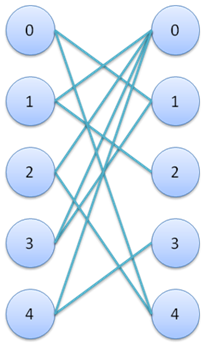
\includegraphics[scale=0.5]{transform.png}\\
建立一个二分图,$X$集合每个顶点代表$0,1,\cdots,N-1$的$N$个整数,$Y$集合每个顶点为对应的$N$个整数。$X$集合的第$i$个顶点向其环上距离为$D_i$的$Y$集合中的两个顶点连一条边。\\
一个合法的变换序列应是$0,1,\cdots,N-1$的一个排列。\\
【算法描述】\\
按照解法3证明中的描述,我们可以预处理所有已经确定的匹配,并在图中删去。对于剩下的每个环,只需从序号最小的点开始深度优先搜索,并进行匹配即可。\\
【算法证明】\\
【证明同解法3】\\
【复杂度分析】\\
预处理的时间复杂度为$O(N)$,深度优先搜索的时间复杂度为$O(N)$,所以总时间复杂度为$O(N)$。
\begin{lstlisting}[language=c++,breaklines=true] 
include <iostream>
include <fstream>
include <cstdlib>
include <cmath>
include <cstring>

using namespace std; 

const int maxN = 20001, maxM = maxN * 4;

struct edge {
    edge* next;
    int t;
} *v[maxN], e[maxM];

int n;
int ec;
int mat[maxN];
int stack[maxN];
int s[maxN][2];
int deg[maxN];
bool nuked[maxN];

inline void addEdge(int a, int b) {
    e[++ec].next = v[a];
    v[a] = e + ec;
    v[a]->t = b;

    e[++ec].next = v[b];
    v[b] = e + ec;
    v[b]->t = a;

    ++deg[b];
    mat[b] = a;
}

void init() {
    ifstream fin("transform.in");
    fin >> n;

    int i, d, t1, t2;

    for (i = 1; i <= n; ++i) {
        fin >> d;

        t1 = i + d;
        if (t1 > n){
		t1 -= n;
	} 

        t2 = i - d;
        if (t2 < 1){
		t2 += n;
	} 

        if (t1 < t2){
		s[i][0] = t1;
		s[i][1] = t2;
	}else{
		s[i][0] = t2;
		s[i][1] = t1;
	}

        addEdge(i, s[i][1] += n);
        addEdge(i, s[i][0] += n);
        deg[i] = 2;
    }

    fin.close();
}

void noAnswer() { 
	printf("No Answer\n"); 
	exit(0); 
}

inline void match(int i,int j) {
	mat[i] = j; 
	mat[j] = i; 
}

void prune() { 
	int stop = 0,i,j; 

	for (i = 1;i <= n; i++) { 
		if (deg[i + n] == 0){
			noAnswer(); 
		}else if(deg[i + n] == 1){
			stack[++stop] = i + n; 
		}
	}

	while(stop){ 
		i = stack[stop--]; 
		nuked[i] = true; 

		for (edge *e=v[i];e;e=e->next) { 
			j = e->t; 
			if (!nuked[j]){
				break; 
			} 
		} 

		match(i,j); 
		i = j; 
		nuked[i] = true; 

		for (edge *e=v[i];e;e=e->next) { 
			j = e->t; 
			if (!nuked[j]) { 
				deg[j]--; 
				if(deg[j] == 0){
					noAnswer(); 
				}else if(deg[j] == 1){
					stack[++stop] = j; 
				} 
			} 
		} 
	} 
}

void dfs(int i,bool s) { 
	nuked[i] = true; 
	int j; 

	for (edge *e=v[i];e;e=e->next) { 
		j = e->t; 
		if(!nuked[j]){ 
			dfs(j,!s); 
			if(s){
				match(i,j); 
			}
			break; 
		} 
	} 
}

void solve() { 
	prune(); 
	for (int i=1;i <= n;i++) { 
		if (!nuked[i]){
			dfs(i,true); 
		} 
	}
}

void print() {
    ofstream fout("transform.out");

    int i;
    for(i = 1; i < n; i++){
	    fout << mat[i] - n - 1 << " ";
    }

    fout << mat[i] - n - 1 << "\n";
    fout.close();
}

int main() {
    init();
    solve();
    print();
    return 0;
}
\end{lstlisting}

\chapter{stack}
\section{expr}
expr-csp-j-2022-3\\
【题目描述】\\
逻辑表达式是计算机科学中的重要概念和工具,包含逻辑值、逻辑运算、逻辑运算
优先级等内容。\\
在一个逻辑表达式中,元素的值只有两种可能:0 (表示假)和1 (表示真)。元素
之间有多种可能的逻辑运算,本题中只需考虑如下两种:“与”(符号为\&)和“或”(符
号为|)。其运算规则如下:\\
0\&0 = 0\&1 = 1\&0 = 0,1\&1 = 1;\\
0|0 = 0,0|1 = 1|0 = 1|1 = 1。\\
在一个逻辑表达式中还可能有括号。规定在运算时,括号内的部分先运算;两种运
算并列时,\& 运算优先于| 运算;同种运算并列时,从左向右运算。\\
比如,表达式0|1\&0 的运算顺序等同于0|(1\&0) ;表达式0\&1\&0|1 的运算顺序等
同于((0\&1)\&0)|1。\\
此外,在C++ 等语言的有些编译器中,对逻辑表达式的计算会采用一种“短路”
的策略。:在形如a\&b 的逻辑表达式中,会先计算a 部分的值,如果a = 0 ,那么整个
逻辑表达式的值就一定为0,故无需再计算b 部分的值;同理,在形如a|b 的逻辑表达
式中,会先计算a 部分的值,如果a = 1 ,那么整个逻辑表达式的值就一定为1,无需
再计算b 部分的值。\\
现在给你一个逻辑表达式,你需要计算出它的值,并且统计出在计算过程中,两种
类型的“短路”各出现了多少次。需要注意的是,如果某处“短路”包含在更外层被“短
路”的部分内则不被统计,如表达式1|(0\&1) 中,尽管0\&1 是一处“短路”,但由于外
层的1|(0\&1) 本身就是一处“短路”,无需再计算0\&1 部分的值,因此不应当把这里的
0\&1 计入一处“短路”。\\
【输入格式】\\
从文件expr.in 中读入数据。\\
输入共一行,一个非空字符串s 表示待计算的逻辑表达式。\\
【输出格式】\\
输出到文件expr.out 中。\\
输出共两行,第一行输出一个字符0 或1 ,表示这个逻辑表达式的值;第二行输
出两个非负整数,分别表示计算上述逻辑表达式的过程中,形如a/\&b 和a|b 的“短路”
各出现了多少次。\\
【样例1 输入】\\
0\&(1|0)|(1|1|1\&0)\\
【样例1 输出】\\
1\\
1 2\\
【样例1 解释】\\
该逻辑表达式的计算过程如下,每一行的注释表示上一行计算的过程:\\
0\&(1|0)|(1|1|1\&0)\\
=(0\&(1|0))|((1|1)|(1\&0)) //用括号标明计算顺序\\
=0|((1|1)|(1\&0)) //先计算最左侧的\&,是一次形如a\&b的“短路”\\
=0|(1|(1\&0)) //再计算中间的|,是一次形如a|b的“短路”\\
=0|1 //再计算中间的|,是一次形如a|b的“短路”\\
=1\\
【样例2 输入】\\
(0|1\&0|1|1|(1|1))\&(0\&1\&(1|0)|0|1|0)\&0\\
【样例2 输出】\\
0\\
2 3
\begin{lstlisting}[language=C++]
include <iostream>
include <fstream>
include <stack>
include <cstring>
using namespace std;

struct node {
    int v; 
    int y; 
    int h; 
};

int main() {
    ifstream fin("expr.in");
    ofstream fout("expr.out");

    char s[1000002];
    stack<char> q;
    stack<node> n; 

    fin >> s;
    int l = strlen(s);
    s[l] = ')'; 
    q.push('(');

    for (int i = 0; i <= l; i++) {
        if (s[i] == '(') {
            q.push(s[i]);
        }
        else if (s[i] == '0' || s[i] == '1') {
            node temp;
            temp.v = s[i] - '0';
            temp.y = 0;
            temp.h = 0;
            n.push(temp);
        }
        else {
            bool fff = false;
            if (s[i] == ')') {
                fff = true;
                if (q.top() == '(') {
                    q.pop();
                }
                else {
                while (!n.empty() && !q.empty() && 
                (q.top() == '&' || q.top() == '|')) {
                        char z = q.top();
                        q.pop();
                        node a = n.top();
                        n.pop();
                        node b = n.top();
                        n.pop();
                        node temp;
                        temp.y = b.y;
                        temp.h = b.h;
                        if (z == '&') {
                            if (b.v == 0) temp.y++;
                            else {
                                temp.y += a.y;
                                temp.h += a.h;
                            }
                            temp.v = a.v & b.v;
                        }
                        if (z == '|') {
                            if (b.v == 1) temp.h++;
                            else {
                                temp.h += a.h;
                                temp.y += a.y;
                            }
                            temp.v = a.v | b.v;
                        }
                        n.push(temp);
                    }
                    q.pop();
                }
            }
            if (!n.empty() && !q.empty()) {
            while ((q.top() == '&' && (s[i] == '&' || s[i] == '|')) || 
            (q.top() == '|' && s[i] == '|')) {
                    char z = q.top();
                    q.pop();
                    node a = n.top();
                    n.pop();
                    node b = n.top();
                    n.pop();
                    node temp;
                    temp.y = b.y;
                    temp.h = b.h;
                    if (z == '&') {
                        if (b.v == 0) temp.y++;
                        else {
                            temp.y += a.y;
                            temp.h += a.h;
                        }
                        temp.v = a.v & b.v;
                    }
                    if (z == '|') {
                        if (b.v == 1) temp.h++;
                        else {
                            temp.h += a.h;
                            temp.y += a.y;
                        }
                        temp.v = a.v | b.v;
                    }
                    n.push(temp);
                }
            }
            if (fff == false)
                q.push(s[i]);
        }
    }
    
    fout << n.top().v << endl;
    fout << n.top().y << ' ' << n.top().h << endl;

    fin.close();
    fout.close();

    return 0;
}
\end{lstlisting}

\section{noip2002-1}
NOIP 2002 普及组第一题:级数求和\\
题目描述\\
已知:$S_n= 1+\dfrac{1}{2}+\dfrac{1}{3}+…+\dfrac{1}{n}$。显然对于任意一个整数 $k$,当 $n$ 足够大的时候,$S_n>k$。
现给出一个整数 $k$,要求计算出一个最小的 $n$,使得 $S_n>k$。\\
输入格式\\
一个正整数 $k$。\\
输出格式\\
一个正整数 $n$。\\
样例输入\\
1\\
样例输出\\
2\\
【数据范围】\\
对于 $100\%$ 的数据,$1\le k \le 15$。\\
解:\\
\begin{lstlisting}[language=c++,breaklines=true]
include <iostream>

using namespace std;

int main(){
	int k;
	cin>>k;
	double s = 0.0;
	int n = 0;
	while(s <= k){
		n++;
		s += 1.0/n;
	}
	cout<<n<<endl;
}
\end{lstlisting}

\section{bubbleSort}
\begin{lstlisting}[language=C++]
include <iostream>
include <vector>
using namespace std;

vector<int> arr = {3,1,5,9,7};

void bubbleSort(vector<int>& arr){
	int n = arr.size();
	for(int i = 0; i < n - 1; i++){
		for(int j = 0; j < n - i - 1; j++){
			if(arr[j] > arr[j + 1]){
				swap(arr[j],arr[j+1]);
			}
		}
	}
}

void printArr(){
	int n = arr.size();
	for(int i = 0; i < n; i++){
		cout<<arr[i]<<',';
	}
	cout<<endl;
}

int main(){
	printArr();
	bubbleSort(arr);
	printArr();
}
\end{lstlisting}

\section{candy}
candy-csp-j-2021-2\\
【题目背景】\\
红太阳幼儿园的小朋友们开始分糖果啦!\\
【题目描述】\\
红太阳幼儿园有$n$个小朋友,你是其中之一。保证$n\geq2$。\\
有一天你在幼儿园的后花园里发现无穷多颗糖果,你打算拿一些糖果回去分给幼儿
园的小朋友们。\\
由于你只是个平平无奇的幼儿园小朋友,所以你的体力有限,至多只能拿$R$块糖
回去。\\
但是拿的太少不够分的,所以你至少要拿$L$块糖回去。保证$n\leq L\leq R$。\\
也就是说,如果你拿了$k$块糖,那么你需要保证$L\leq k\leq R$。\\
如果你拿了$k$块糖,你将把这$k$块糖放到篮子里,并要求大家按照如下方案分糖
果:只要篮子里有\dotuline{不少于}$n$块糖果,幼儿园的所有$n$个小朋友(包括你自己)都从篮子
中拿走\dotuline{恰好}一块糖,直到篮子里的糖数量\dotuline{少于}$n$块。此时篮子里剩余的糖果均归你所有
——这些糖果是\dotuline{作为你搬糖果的奖励}。\\
作为幼儿园高质量小朋友,你希望让\dotuline{作为你搬糖果的奖励}的糖果数量(\dotuline{而不是你最后获得的总糖果数量}!)尽可能多;因此你需要写一个程序,依次输入$n, L, R$,并输出你最多能获得多少作为你搬糖果的奖励的糖果数量。\\
【输入格式】\\
从文件 candy.in 中读入数据。\\
输入一行,包含三个正整数 $n, L, R$,分别表示小朋友的个数、糖果数量的下界和上界。\\
【输出格式】\\
输出到文件 candy.out 中。\\
输出一行一个整数,表示你最多能获得的\dotuline{作为你搬糖果的奖励}的糖果数量。\\
【样例 1 输入】\\
7 16 23\\
【样例 1 输出】\\
6\\
【样例 1 解释】\\
拿$k = 20$ 块糖放入篮子里。\\
篮子里现在糖果数 $20 \geq n = 7$,因此所有小朋友获得一块糖;\\
篮子里现在糖果数变成 $13 \geq n = 7$,因此所有小朋友获得一块糖;\\
篮子里现在糖果数变成 $6 < n = 7$,因此这 6 块糖是\dotuline{作为你搬糖果的奖励}。
容易发现,你获得的\dotuline{作为你搬糖果的奖励}的糖果数量不可能超过 6 块(不然,篮子
里的糖果数量最后仍然不少于 n,需要继续每个小朋友拿一块),因此答案是 6。\\
【样例 2 输入】\\
10 14 18\\
【样例 2 输出】\\
8\\
【样例 2 解释】\\
容易发现,当你拿的糖数量 k 满足 $14 = L \leq k \leq R = 18$ 时,所有小朋友获得一块
糖后,剩下的 k − 10 块糖总是\dotuline{作为你搬糖果的奖励}的糖果数量,因此拿 $k = 18$ 块是最
优解,答案是 8。\\
【数据范围】\\
\begin{tabular}{|c|c|c|c|}
  \hline
  测试点 &  $n\leq$ & $R\leq$ & $R-L\leq$\\
  \hline
  1 & 2 & 5 & 5\\
  \hline
  2 & 5 & 10 & 10\\
  \hline
  3 & $10^3$ & $10^3$ & $10^3$\\
  \hline
  4 & $10^5$ & $10^5$ & $10^5$\\
  \hline
  5 & & & 0\\
  \cline{1-1}
  \cline{4-1}
  6 & $10^3$ & & $10^3$\\
  \cline{1-1}
  \cline{2-1}
  \cline{4-1}
  7 & $10^5$ & $10^9$ & $10^5$\\
  \cline{1-1}
  \cline{2-1}
  \cline{4-1}
  8 & & & \\
  \cline{1-1}
  9 & $10^9$ & & $10^{9}$\\
  \cline{1-1}
  10 & & &\\
  \hline
\end{tabular}\\
对于所有数据,保证 $2 \leq n \leq L \leq R \leq 10^9$\\
解:\\
\begin{tabular}{|c|c|c|c|c|}
\hline
1 & input &7 16 23 & $n, L, R$ & 小朋友的个数、糖果数量的下界和上界\\
\hline
2 & output & 6 & k & 你最多能获得的糖果数量\\
\hline
\end{tabular}\\
\begin{lstlisting}[language=C++]
include <iostream>
include <fstream>

using namespace std;

int main(){
	ifstream fin("candy.in");
	ofstream fout("candy.out");
	int n,l,r;
	int k;
	fin>>n>>l>>r;
	if(l<n*(r/n)&&n*(r/n)<r){
		k = n * (r/n) -1-n*(r/n-1);
	}else if(n*(r/n)<l){
		k = r - n;
	}
	fout<<k;
	return 0;
}
\end{lstlisting}

\section{后缀自动机}

\section{dag}
Directed Acyclic Graph 有向无环图

\section{最大流问题}
问题描述:在一个有向图中,求从源点到汇点的最大流。\\
解法思路:\\
使用 Edmonds-Karp 算法(BFS 实现的 Ford-Fulkerson 方法)。
维护流网络,并不断寻找增广路径。\\
代码模板:
\begin{lstlisting}[language=C++]
include <bits/stdc++.h>
using namespace std;

const int MAXN = 1000; // 最大节点数
const int INF = INT_MAX;

struct Edge {
    int v, cap, flow, rev;
};

class MaxFlow {
public:
    vector<Edge> adj[MAXN];

    void addEdge(int u, int v, int cap) {
        adj[u].push_back({v, cap, 0, (int)adj[v].size()});
        adj[v].push_back({u, 0, 0, (int)adj[u].size() - 1});
    }

    int bfs(int s, int t, vector<int>& parent) {
        fill(parent.begin(), parent.end(), -1);
        queue<pair<int, int>> q;
        q.push({s, INF});
        parent[s] = -2;

        while (!q.empty()) {
            int cur = q.front().first;
            int flow = q.front().second;
            q.pop();

            for (auto& edge : adj[cur]) {
                if (parent[edge.v] == -1 && edge.flow < edge.cap) {
                    parent[edge.v] = cur;
                    int new_flow = min(flow, edge.cap - edge.flow);
                    if (edge.v == t) return new_flow;
                    q.push({edge.v, new_flow});
                }
            }
        }
        return 0;
    }

    int maxFlow(int s, int t) {
        int flow = 0, new_flow;
        vector<int> parent(MAXN);
        while (new_flow = bfs(s, t, parent)) {
            flow += new_flow;
            int cur = t;
            while (cur != s) {
                int prev = parent[cur];
                for (auto& edge : adj[prev]) {
                    if (edge.v == cur) {
                        edge.flow += new_flow;
                        break;
                    }
                }
                for (auto& edge : adj[cur]) {
                    if (edge.v == prev) {
                        edge.flow -= new_flow;
                        break;
                    }
                }
                cur = prev;
            }
        }
        return flow;
    }
};

// 示例用法
int main() {
    MaxFlow mf;
    int n; // 节点数量
    // 输入图的边
    // mf.addEdge(u, v, capacity);
    // ...
    cout << "最大流: " << mf.maxFlow(source, sink) << endl;
    return 0;
}
\end{lstlisting}

\section{动态规划(01 背包问题)}
问题描述:给定一些物品,每个物品有重量和价值,求在不超过背包容量的情况下可以获得的最大价值。\\
解法思路:\\
使用动态规划,状态转移方程为 dp[i][j] = max(dp[i-1][j], dp[i-1][j-weight[i]] + value[i])。\\
代码模板:
\begin{lstlisting}[language=C++]
include <bits/stdc++.h>
using namespace std;

const int MAXN = 100; // 最大物品数
const int MAXW = 10000; // 最大背包容量

int dp[MAXN][MAXW];

int knapsack(int n, int W, vector<int>& weight, vector<int>& value) {
    for (int i = 0; i <= n; i++) {
        for (int w = 0; w <= W; w++) {
            if (i == 0 || w == 0)
                dp[i][w] = 0;
            else if (weight[i - 1] <= w)
                dp[i][w] = max(dp[i - 1][w], dp[i - 1][w - weight[i - 1]] + value[i - 1]);
            else
                dp[i][w] = dp[i - 1][w];
        }
    }
    return dp[n][W];
}

// 示例用法
int main() {
    int n, W; // 物品数量和背包容量
    vector<int> weight(n), value(n);
    // 输入物品的重量和价值
    // ...
    
    cout << "最大价值: " << knapsack(n, W, weight, value) << endl;
    return 0;
}
\end{lstlisting}

\section{binarySearch}
问题描述:在一个有序数组中查找某个元素,或在某个条件下寻找最优解。\\
解法思路:\\
使用二分查找快速定位目标元素或满足条件的值。\\
代码模板:
\begin{lstlisting}[language=C++]
include <bits/stdc++.h>
using namespace std;

int binarySearch(const vector<int>& arr, int target) {
    int left = 0, right = arr.size() - 1;
    while (left <= right) {
        int mid = left + (right - left) / 2;
        if (arr[mid] == target)
            return mid; // 找到目标
        else if (arr[mid] < target)
            left = mid + 1;
        else
            right = mid - 1;
    }
    return -1; // 未找到
}

// 示例用法
int main() {
    vector<int> arr = {1, 2, 3, 4, 5};
    int target = 3;
    int index = binarySearch(arr, target);
    cout << "元素 " << target << (index != -1 ? " 在索引 " + to_string(index) : " 未找到") << endl;
    return 0;
}
\end{lstlisting}

\section{排序问题}
问题描述:对给定的一组数据进行排序。例如:给定一个包含整数的数组,将其从小到大排序并输出。\\
解法思路:\\
可以使用的算法有冒泡排序、插入排序、选择排序、快速排序、归并排序等。以快速排序为例:\\
代码模板:
\begin{lstlisting}[language=C++]
include <iostream>
include <vector>

void quickSort(std::vector<int>& arr, int left, int right) {
    if (left >= right) return;
    int pivot = arr[(left + right) / 2];
    int i = left, j = right;
    while (i <= j) {
        while (arr[i] < pivot) i++;
        while (arr[j] > pivot) j--;
        if (i <= j) {
            std::swap(arr[i], arr[j]);
            i++;
            j--;
        }
    }
    quickSort(arr, left, j);
    quickSort(arr, i, right);
}

int main() {
    std::vector<int> arr = {5, 3, 8, 4, 2};
    quickSort(arr, 0, arr.size() - 1);
    for (int num : arr) {
        std::cout << num << " ";
    }
    return 0;
}
\end{lstlisting}

\section{live}
live-csp-j-2020-2\\
直播获奖(live)\\
【题目描述】\\
NOI2130即将举行。为了增加观赏性,CCF决定逐一评出每个选手的成
绩,并直播即时的获奖分数线。本次竞赛的获奖率为$w\%$,即当前排名前$w\%$的选手的最低成绩就是即时的分数线。\\
更具体地, 若当前已评出了$p$个选手的成绩, 则当前计划获奖人数为
$max(1,\lfloor p\times w\%\rfloor)$, 其中$w$是获奖百分比, $\lfloor x \rfloor$表示对$x$向下取整,
$max(x,y)$ 表示 $x$ 和 $y$中较大的数。如有选手成绩相同,则所有成绩并列的
选手都能获奖,因此实际获奖人数可能比计划中多。\\
作为评测组的技术人员,请你帮CCF写一个直播程序。\\
【输入格式】\\
输入文件名为 live.in。\\
第 1 行两个正整数$n,w$。 分别代表选手总数与获奖率。\\
第 2 行有$n$个非负整数,依次代表逐一评出的选手成绩。\\
【输出格式】\\
输出文件名为 live.out。\\
只有一行,包含$n$个非负整数,依次代表选手成绩逐一评出后,即时的获
奖分数线。 相邻两个整数间用一个空格分隔。\\
【样例 1 输入】\\
10 60\\
200 300 400 500 600 600 0 300 200 100\\
【样例 1 输出】\\
200 300 400 400 400 500 400 400 300 300\\
解:
\begin{lstlisting}[language=C++,breaklines = true]
include <iostream>
include <fstream>

using namespace std;

int n,w,x;
int a[610];

int main(){
	ifstream fin("live.in");
	ofstream fout("live.out");
	fin>>n>>w;

	int k;
	int ans;
	for(int i = 1; i <= n; i++){
		fin>>x;
		a[x]++;
		k = max(1,int(i * w / 100.0));
		ans = 0;
		for(int j = 600;j >= 0; j--){
			if(ans + a[j] < k){
				ans += a[j];
			} else {
				fout<<j<<" ";
				break;
			}
		}
	}
	fout<<"\n";

	fin.close();
	fout.close();
	return 0;
}
\end{lstlisting}

\section{number}
number-csp-j-2020-4\\
方格取数number\\
【题目描述】\\
设有$n\times m$的方格图,每个方格中都有一个整数。现有一只小熊, 想从图
的左上角走到右下角,每一步只能向上、向下或向右走一格, 并且不能重复经
过已经走过的方格,也不能走出边界。小熊会取走所有经过的方格中的整数,
求它能取到的整数之和的最大值。\\
【输入格式】\\
输入文件名为 number.in。\\
第 1 行两个正整数$n,m$。\\
接下来$n$行每行$m$个整数, 依次代表每个方格中的整数。\\
【输出格式】\\
输入文件名为 number.out。\\
一个整数,表示小熊能取到的整数之和的最大值。\\
【样例 1 输入】\\
3 4\\
1 -1 3 2\\
2 -1 4 -1\\
-2 2 -3 -1\\
【样例 1 输出】\\
9\\
【样例 1 解释】\\
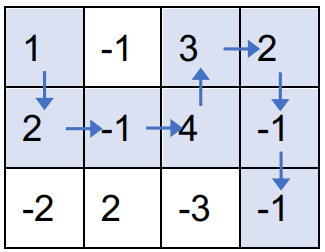
\includegraphics[scale=0.5]{num.png}\\
按上述走法,取到的数之和为 1 + 2 + (-1) + 4 + 3 + 2 + (-1) + (-1) = 9,可
以证明为最大值。\\
解:
\begin{lstlisting}[language=C++,breaklines = true]
include <iostream>
include <fstream>

using namespace std;

int n,m;
const long long minNum = -1e18;
long long gridValue[1005][1005];
long long memorizationTable[1005][1005][2];

inline long long maxNum(long long p, long long q, long long r){
	return p > q ? (p > r ? p : r) : (q > r ? q : r);
}

long long dfs(int x,int y,int from){
	if(x < 1 && x > n || y < 1 && y > m){
		return minNum;
	}

	if(memorizationTable[x][y][from] != minNum){
		return memorizationTable[x][y][from];
	}

	if(from == 0){
		memorizationTable[x][y][from] = maxNum(dfs(x + 1, y, 0),dfs(x, y - 1, 0),dfs(x, y - 1, 1)) + gridValue[x][y];
	}else{
		memorizationTable[x][y][from] = maxNum(dfs(x - 1, y, 1),dfs(x, y - 1, 0),dfs(x, y - 1, 1)) + gridValue[x][y];
	}

	return memorizationTable[x][y][from];
}

int main(){
	ifstream fin("number.in");
	ofstream fout("number.out");

	fin>>n>>m;
	for(int i = 1; i <= n; i++){
		for(int j = 1; j <= m; j++){
			fin>>gridValue[i][j];
			memorizationTable[i][j][0] = memorizationTable[i][j][1] = minNum;
		}
	}
	memorizationTable[1][1][0] = memorizationTable[1][1][1] = minNum;

	fout<<dfs(n,m,1)<<endl;
	fin.close();
	fout.close();
	return 0;
}
\end{lstlisting}

\section{expr}
expr-csp-j-2020-3\\
表达式(expr)\\
【题目描述】\\
小$C$热衷于学习数理逻辑。有一天,他发现了一种特别的逻辑表达式。在
这种逻辑表达式中, 所有操作数都是变量, 且它们的取值只能为0或1,运算
从左往右进行。如果表达式中有括号,则先计算括号内的子表达式的值。特别
的,这种表达式有且仅有以下几种运算:\\
1. 与运算: $a\&b$。当且仅当a和b的值都为1时,该表达式的值为1。其余情况该表达式的值为0。\\
2. 或运算: $a|b$。当且仅当a和b的值都为0时,该表达式的值为0。其余情况该表达式的值为 1。\\
3. 取反运算: $!a$。当且仅当$a$的值为0时,该表达式的值为 1。其余情况该表达式的值为 0。\\
小 C 想知道,给定一个逻辑表达式和其中每一个操作数的初始取值后, 再
取反某一个操作数的值时,原表达式的值为多少。\\
为了化简对表达式的处理,我们有如下约定:\\
表达式将采用后缀表达式的方式输入。后缀表达式的定义如下:\\
1. 如果$E$是一个操作数,则$E$的后缀表达式是它本身。\\
2. 如果$E$是$E_1\quad op\quad E_2$形式的表达式,其中$op$是任何二元操作符, 且优
先级不高于$E_1,E_2$中括号外的操作符, 则$E$的后缀式为${E_1}'{E_2}'op$,其中${E_1}',{E_2}'$分别为$E_1,E_2$的后缀式。\\
3. 如果$E$是$(E_1)$形式的表达式,则$(E_1)$的后缀式就是$E$的后缀式。\\
同时为了方便, 输入中:\\
a) 与运算符(\&)、或运算符(|)、取反运算符(!)的左右均有一个空格,
但表达式末尾没有空格。\\
b) 操作数由小写字母 x 与一个正整数拼接而成,正整数表示这个变量的下
标。例如: $x10$, 表示下标为10的变量$x_{10}$。数据保证每个变量在表达
式中出现恰好一次。\\
【输入格式】\\
输入文件名为 expr.in。\\
第一行包含一个字符串$s$,表示上文描述的表达式。\\
第二行包含一个正整数$n$,表示表达式中变量的数量。表达式中变量的下
标为 $1,2, \cdots , n$。\\
第三行包含$n$个整数, 第$i$个整数表示变量$x_i$的初值。\\
第四行包含一个正整数$q$,表示询问的个数。\\
接下来$q$行,每行一个正整数,表示需要取反的变量的下标。注意,每一
个询问的修改都是临时的,即之前询问中的修改不会对后续的询问造成影响。
数据保证输入的表达式合法。 变量的初值为 0 或 1。\\
【输出格式】\\
输出文件名为 expr.out。\\
输出一共有 𝑞 行,每行一个 0 或 1,表示该询问下表达式的值。\\
【样例 1 输入】\\
x1 x2 \& x3 |\\
3\\
1 0 1\\
3\\
1\\
2\\
3\\
【样例 1 输出】\\
1 1 0\\
【样例 1 解释】\\
该后缀表达式的中缀表达式形式为 $(𝑥1 \& 𝑥2) | 𝑥3$。\\
对于第一次询问,将 𝑥1 的值取反。此时,三个操作数对应的赋值依次为
0, 0, 1。原表达式的值为 $(0 \& 0)$ | 1 = 1。\\
对于第二次询问,将 𝑥2 的值取反。此时,三个操作数对应的赋值依次为
1, 1, 1。原表达式的值为 $(1 \& 1) | 1 = 1$。\\
对于第三次询问,将 𝑥3 的值取反。此时,三个操作数对应的赋值依次为
1, 0, 0。原表达式的值为 $(1 \& 0) | 0 = 0$。\\
解:\\
【条件分析】\\
\begin{tabular}{|c|c|}
  \hline
  条件编号 & 条件描述 \\
  \hline
  1 & 表达式中的操作数只能取值为0或1 \\
  \hline
  2 & 运算从左往右进行\\
  \hline
  3 & 如果表达式中有括号,则先计算括号内的子表达式的值 \\
  \hline
  4 & 表达式中只包含三种运算符:与运算(\&)、或运算( \\
  \hline
  5 & 与运算(\&)的结果为1的条件是,两个操作数的值都为1;否则结果为0\\
  \hline
  6 & 或运算(\\
  \hline
  7 & 取反运算(!)的结果为1的条件是,操作数的值为0;否则结果为0\\
  \hline
  8 & 表达式采用后缀表达式的方式输入,即运算符在操作数之后\\
  \hline
  9 & 后缀表达式的定义:\\
  \hline
\end{tabular}

\section{point}
point-csp-2022-4\\
【题目描述】\\
在一个二维平面内,给定$n$个整数点 ($x_i$, $y_i$),此外你还可以自由添加$k$个整数点。你在自由添加$k$个点后,还需要从$n+k$个点中选出若干个整数点并组成一个序列,使得序列中任意相邻两点间的欧几里得距离恰好为1而且横坐标、纵坐标值均单调不减,即$x_{i+1} −x_i=1$, $y_{i+1}=y_i$或$y_{i+1}−y_i=1$, $x_{i+1}=x_i$。请给出满足条件的序列的最大长度。\\
【输入格式】\\
从文件 point.in 中读入数据。\\
第一行两个正整数$n,k$分别表示给定的整点个数、可自由添加的整点个数。接下来$n$行,第i行两个正整数$x_i$, $y_i$表示给定的第i个点的横纵坐标。\\
【输出格式】\\
输出到文件 point.out 中。\\
输出一个整数表示满足要求的序列的最大长度。\\
【样例 1 输入】\\
\begin{tabular}{|c|}
\hline
8 2\\
3 1\\
3 2\\
3 3\\
3 6\\
1 2\\
2 2\\
5 5\\
5 3\\
\hline
\end{tabular}\\
【样例 1 输出】\\
\begin{tabular}{|c|}
\hline
8\\
\hline
\end{tabular}\\
【样例 2 输入】\\
\begin{tabular}{|c|}
\hline
4 100\\
10 10\\
15 25\\
20 20\\
30 30\\
\hline
\end{tabular}\\
【样例 2 输出】\\
\begin{tabular}{|c|}
\hline
103\\
\hline
\end{tabular}\\
解:
\begin{lstlisting}[language=C++,breaklines=true]
include <iostream>
include <fstream>
include <vector>
include <algorithm>

using namespace std;

int main(){
	ifstream fin("point.in");
	ofstream fout("point.out");

	int n,k;
	fin>>n>>k;
	int ans = 0;

	vector<pair<int,int>> points(n);
	for(int i = 0; i < n; i++){
		int x,y;
		fin>>x>>y;
		points[i] = {x,y};
	}

	sort(points.begin(),points.end());

	vector<vector<int>> dp(n,vector<int>(k + 1,0));
	for(int i = 0; i < n; i++){
		for(int j = 0; j <= k; j++){
			dp[i][j] = j + 1;
			for(int t = 0; t < i; t++){
				pair<int,int> &A = points[i];
				pair<int,int> &B = points[t];
				int d = A.first - B.first + A.second - B.second - 1;
				if(A.second >= B.second){
					if(j >= d){
						dp[i][j] = max(dp[i][j],dp[t][j - d] + d + 1);
					}
				}
			}
			ans = max(ans,dp[i][j]);
		}
	}

	fout<<ans<<endl;
	fin.close();
	fout.close();
	return 0;
}
\end{lstlisting}

\section{fruit}
fruit-csp-2021-4\\
小熊的果篮(fruit)\\
【题目描述】\\
小熊的水果店里摆放着一排n个水果。每个水果只可能是苹果或桔子,从左到右依
次用正整数 1、 2、 3、 ……、 n 编号。连续排在一起的同一种水果称为一个“块”。小熊
要把这一排水果挑到若干个果篮里,具体方法是:每次都把每一个“块”中最左边的水
果同时挑出,组成一个果篮。重复这一操作,直至水果用完。注意,每次挑完一个果篮
后,“块”可能会发生变化。比如两个苹果“块”之间的唯一桔子被挑走后,两个苹果
“块”就变成了一个“块”。请帮小熊计算每个果篮里包含的水果。\\
【输入格式】\\
从文件 fruit.in 中读入数据。\\
输入的第一行包含一个正整数 n,表示水果的数量。\\
输入的第二行包含 n 个空格分隔的整数,其中第 i 个数表示编号为 i 的水果的种
类, 1代表苹果, 0代表桔子。\\
【输出格式】\\
输出到文件 fruit.out 中。\\
输出若干行。\\
第 i 行表示第 i 次挑出的水果组成的果篮。从小到大排序输出该果篮中所有水果的
编号,每两个编号之间用一个空格分隔。\\
【样例1输入】\\
\begin{tabular}{|c|}
\hline
12\\
1 1 0 0 1 1 1 0 1 1 0 0\\
\hline
\end{tabular}\\
【样例1输出】\\
\begin{tabular}{|c|}
\hline
1 3 5 8 9 11\\
2 4 6 12\\
7\\
10\\
\hline
\end{tabular}\\
【样例 1 解释】\\
这是第一组数据的样例说明。\\
所有水果一开始的情况是 1 1 0 0 1 1 1 0 1 1 0 0 一共有6个块。\\
在第一次挑水果组成果篮的过程中,编号为1 3 5 8 9 11的水果被挑了出来。\\
之后剩下的水果是 1 0 1 1 1 0,一共4个块。\\
在第二次挑水果组成果篮的过程中,编号为2 4 6 12的水果被挑了出来。\\
之后剩下的水果是1 1,只有1个块。\\
在第三次挑水果组成果篮的过程中,编号为7的水果被挑了出来。\\
最后剩下的水果是1,只有1个块。\\
在第四次挑水果组成果篮的过程中,编号为10的水果被挑了出来。\\
解:\\
\begin{lstlisting}[language=C++,breaklines = true]
include <bits/stdc++.h>

define INF 200010

using namespace std;

int n;
set<int> s1, s2; // 两个集合,分别存储元素的下标

int main() {
    ifstream fin("fruit.in");  // 从文件 "fruit.in" 读取输入
    ofstream fout("fruit.out"); // 输出结果到文件 "fruit.out"

    fin >> n; // 读取元素数量 n
    s1.clear(); // 清空集合 s1
    s2.clear(); // 清空集合 s2
    int q;
    for (int i = 1; i <= n; ++i) {
        fin >> q; // 读取输入元素 q
        if (q) s1.insert(i); // 若 q 非零,将当前下标 i 插入集合 s1
        else s2.insert(i);    // 若 q 为零,将当前下标 i 插入集合 s2
    }
    s1.insert(INF); // 在集合 s1 中插入 INF,用于防止集合为空
    s2.insert(INF); // 在集合 s2 中插入 INF,用于防止集合为空
    int nw = 0;
    bool p = *s1.begin() < *s2.begin() ? 0 : 1; // 根据两个集合的最小值确定 p 值,表示当前删的是哪个集合

    while (!p && s1.size() > 1 || p && s2.size() > 1) {
        if (!p) {
            nw = *s1.upper_bound(nw); // 找到集合 s1 中下一个大于 nw 的元素
            if (nw == INF) {
                nw = 0;
                p = *s1.begin() < *s2.begin() ? 0 : 1; // 若找不到下一个元素,重新确定 p 值
                fout << endl; // 换行
                continue;
            }
            fout << nw << ' '; // 输出 nw 并删除它
            s1.erase(nw);
            p = !p; // 切换到另一个集合
        } else {
            nw = *s2.upper_bound(nw);
            if (nw == INF) {
                nw = 0;
                p = *s1.begin() < *s2.begin() ? 0 : 1;
                fout << endl;
                continue;
            }
            fout << nw << ' ';
            s2.erase(nw);
            p = !p;
        }
    }
    fout << ""<<endl; // 输出最后一个果篮并换行
    while (s1.size() > 1) fout << *s1.begin() << endl, s1.erase(*s1.begin()); // 逐行输出 s1 剩余元素
    while (s2.size() > 1) fout << *s2.begin() << endl, s2.erase(*s2.begin()); // 逐行输出 s2 剩余元素

    return 0;
}
\end{lstlisting}

\section{solve}
csp-j-2021-13\\
\begin{lstlisting}[language=C++,breaklines = true]
include <iostream>

using namespace std;

int solve(int n){
	if(n <= 1){
		return 1;
	}else if(n >= 5){
		return n * solve(n-2); 2*solve(1)=2 solve(1)=1
	}else{
		return n*solve(n-1);
	}
	return 0;
}

int main(){
	int i = 7;
	int result = solve(7);
	cout<<result<<endl;
	return 0;
}
\end{lstlisting}

\section{network}
network-csp-2021-3\\
【题目描述】\\
TCP/IP 协议是网络通信领域的一项重要协议。今天你的任务,就是尝试利用这个
协议,还原一个简化后的网络连接场景。\\
在本问题中,计算机分为两大类:服务机(Server)和客户机(Client)。服务机
负责建立连接,客户机负责加入连接。\\
需要进行网络连接的计算机共有 n 台,编号为 1 ∼ n ,这些机器将按编号递增的顺
序,依次发起一条建立连接或加入连接的操作。\\
每台机器在尝试建立或加入连接时需要提供一个地址串。服务机提供的地址串表示
它尝试建立连接的地址,客户机提供的地址串表示它尝试加入连接的地址。\\
一个符合规范的地址串应当具有以下特征:\\
1、必须形如 a.b.c.d:e 的格式,其中 a, b, c, d, e 均为非负整数;\\
2、 0 ≤ a, b, c, d ≤ 255, 0 ≤ e ≤ 65535;\\
3、 a, b, c, d, e 均不能含有多余的前导 0。\\
相应地,不符合规范的地址串可能具有以下特征:\\
1、不是形如 a.b.c.d:e 格式的字符串,例如含有多于 3 个字符 . 或多于 1 个字
符 : 等情况;\\
2、整数 a, b, c, d, e 中某一个或多个超出上述范围;\\
3、整数 a, b, c, d, e 中某一个或多个含有多余的前导 0 。
例如,地址串 192.168.0.255:80 是符合规范的,但 192.168.0.999:80 、192.168.00.1:10
、 192.168.0.1:088 、 192:168:0:1.233 均是不符合规范的。
如果服务机或客户机在发起操作时提供的地址串不符合规范,这条操作将被直接忽
略。
在本问题中,我们假定凡是符合上述规范的地址串均可参与正常的连接,你无需考
虑每个地址串的实际意义。\\
由于网络阻塞等原因,不允许两台服务机使用相同的地址串,如果此类现象发生,
后一台尝试建立连接的服务机将会无法成功建立连接;除此之外,凡是提供符合规范的
地址串的服务机均可成功建立连接。\\
如果某台提供符合规范的地址的客户机在尝试加入连接时,与先前某台已经成功建
立连接的服务机提供的地址串相同,这台客户机就可以成功加入连接,并称其连接到这
台服务机;如果找不到这样的服务机,则认为这台客户机无法成功加入连接。
请注意,尽管不允许两台不同的服务机使用相同的地址串,但多台客户机使用同样
的地址串,以及同一台服务机同时被多台客户机连接的情况是被允许的。
你的任务很简单:在给出每台计算机的类型以及地址串之后,判断这台计算机的连
接情况。\\
【输入格式】\\
从文件 network.in 中读入数据。\\
第 1 行,一个正整数 n 。\\
接下来 n 行,每行 2 个字符串 op, ad ,按照编号从小到大给出每台计算机的类型
及地址串。\\
其中 op 保证为字符串 Server 或 Client 之一, ad 为一个长度不超过 25 的,仅
由数字、字符 . 和字符 : 组成的非空字符串。\\
每行的两个字符串之间用恰好一个空格分隔开,每行的末尾没有多余的空格。\\
【输出格式】\\
输出到文件 network.out 中。\\
输出共 n 行,每行一个正整数或字符串表示第 i 台计算机的连接状态。其中:\\
如果第 i 台计算机为服务机,则:\\
1. 如果其提供符合规范的地址串且成功建立连接,输出字符串 OK 。\\
2. 如果其提供符合规范的地址串,但由于先前有相同地址串的服务机而无法成功
建立连接,输出字符串 FAIL 。\\
3. 如果其提供的地址串不是符合规范的地址串,输出字符串 ERR 。\\
如果第 i 台计算机为客户机,则:\\
1. 如果其提供符合规范的地址串且成功加入连接,输出一个正整数表示这台客户
机连接到的服务机的编号。\\
2. 如果其提供符合规范的地址串,但无法成功加入连接时,输出字符串 FAIL 。\\
3. 如果其提供的地址串不是符合规范的地址串,输出字符串 ERR 。\\
【样例 1 输入】\\
\begin{tabular}{|c|}
\hline
5\\
192.168.1.1:8080\\
Server 192.168.1.1:8080\\
Client 192.168.1.1:8080\\
Client 192.168.1.1:80\\
Client 192.168.1.1:99999\\
\hline
\end{tabular}\\
【样例 1 输出】\\
\begin{tabular}{|c|}
\hline
OK\\
FAIL\\
1\\
FAIL\\
ERR\\
\hline
\end{tabular}
解:\\

\section{josephus}
josephus-csp-2021\\
(Josephus 问题)有$n$个人围成一个圈,依次标号0至$�n-1$。\\
从0号开始,依次 0, 1, 0, 1, … 交替报数,报到 1 的人会离开,直至圈中只剩下一个人。\\
求最后剩下人的编号。\\
求解方法:\\
解决Josephus问题的经典方法是使用递归或数学公式。\\
可以得到一个递推关系式,用 f(n,m) 表示 n 个人报数,报到 m 时最后剩下的人的编号。\\
递推关系式为:\\
$f(n,m)=(f(n-1,m)+m)\%n$\\
其中,f(1,m) = 0,表示只剩下一个人时的情况。\\
这个关系式的意义是:在 n 个人报数的情况下,\\
第一轮报数时,第一个被淘汰的人的编号为 (f(n-1,m) + m) % n。\\
然后问题转化为 n-1 个人报数的情况,并从下一个人开始重新报数。\\
通过不断递归计算 f(n,m),最终可以得到只剩下最后一个人的编号,即 Josephus 问题的解。\\
解:\\
\begin{lstlisting}[language=c++,breaklines=true]
include <iostream>

using namespace std;

const int MAXN = 1000000; // 最大的人数
int F[MAXN]; // 标记每个人是否被淘汰出圈

int main(){
	int n;
	cin >> n; // 接收输入的人数n
	int i = 0,p = 0,c = 0; // 当前报数的人编号、报数的标记、以及已经被淘汰的人数
	while(c < n - 1){ // 进入一个while循环,循环条件是还未剩下最后一个人
		if(F[i] == 0){ // 判断当前报数的人是否还在圈内,如果F[i]为0,表示该人还在圈内
			if(p){// 判断当前报数标记p的值。p的初始值为0,当p为1时,说明报数到1i,该人将被淘汰
				F[i] = 1; // 将当前报数的人标记为1,表示被淘汰
				c++; // 然后c增加1,表示已经淘汰的人数加1 
			} 
			p^=1; // 将p的值进行异或运算,相当于p取反,即0变成1,1变成0。这样可以实现交替报数的效果
		}
		i = (i + 1) % n; // 更新报数的人的编号i,取余操作确保编号在圈内循环
	}
	int ans = -1; // 定义一个变量ans,用于记录最后剩下的人的编号,初始化为-1
	for(i = 0;i < n;i++) // 遍历数组F,查找最后剩下的人的编号
		if(F[i] == 0) // 如果F[i]为0,表示该人未被淘汰
			ans = i; // 将该人的编号赋值给ans
	cout << ans << endl;
	return 0;
}
\end{lstlisting}

\chapter{dijkstra}
\section{最短路径(Dijkstra 算法)}
问题描述:在一个加权有向图中,求从源点到所有其他点的最短路径。\\
解法思路:\\
使用 Dijkstra 算法,适用于正权重的图。\\
代码模板:
\begin{lstlisting}[language=C++]
include <bits/stdc++.h>
using namespace std;

const int MAXN = 1000; // 最大节点数
const int INF = INT_MAX;

vector<pair<int, int>> adj[MAXN]; // 邻接表:pair<邻接节点, 边权>

void dijkstra(int source, vector<int>& dist) {
    dist.assign(MAXN, INF);
    dist[source] = 0;
    priority_queue<pair<int, int>, vector<pair<int, int>>, greater<pair<int, int>>> pq;
    pq.push({0, source}); // {距离, 节点}

    while (!pq.empty()) {
        int d = pq.top().first;
        int u = pq.top().second;
        pq.pop();

        if (d > dist[u]) continue; // 如果已经找到更短的路径,跳过

        for (auto& edge : adj[u]) {
            int v = edge.first, weight = edge.second;
            if (dist[u] + weight < dist[v]) {
                dist[v] = dist[u] + weight;
                pq.push({dist[v], v});
            }
        }
    }
}

// 示例用法
int main() {
    int n, m; // n 为节点数,m 为边数
    // 输入图的边
    // adj[u].push_back({v, weight});
    // ...
    
    vector<int> dist;
    dijkstra(source, dist);
    for (int i = 0; i < n; i++) {
        cout << "从源点到节点 " << i << " 的最短距离: " << dist[i] << endl;
    }
    return 0;
}
\end{lstlisting}

\section{bus}
 [CSP-J 2023] 旅游巴士
 题目描述
小 Z 打算在国庆假期期间搭乘旅游巴士去一处他向往已久的景点旅游。

旅游景点的地图共有 $n$ 处地点,在这些地点之间连有 $m$ 条道路。其中 $1$ 号地点为景区入口,$n$ 号地点为景区出口。我们把一天当中景区开门营业的时间记为 $0$ 时刻,则从 $0$ 时刻起,每间隔 $k$ 单位时间便有一辆旅游巴士到达景区入口,同时有一辆旅游巴士从景区出口驶离景区。

所有道路均只能单向通行。对于每条道路,游客步行通过的用时均为恰好 $1$ 单位时间。

小 Z 希望乘坐旅游巴士到达景区入口,并沿着自己选择的任意路径走到景区出口,再乘坐旅游巴士离开,这意味着他到达和离开景区的时间都必须是 $k$ 的非负整数倍。由于节假日客流众多,小 Z 在旅游巴士离开景区前只想一直沿着景区道路移动,而不想在任何地点(包括景区入口和出口)或者道路上停留。

出发前,小 Z 忽然得知:景区采取了限制客流的方法,对于每条道路均设置了一个
“开放时间”$a _ i$,游客只有不早于 $a _ i$ 时刻才能通过这条道路。

请帮助小 Z 设计一个旅游方案,使得他乘坐旅游巴士离开景区的时间尽量地早。

 输入格式

输入的第一行包含 3 个正整数 $n, m, k$,表示旅游景点的地点数、道路数,以及旅游巴士的发车间隔。

输入的接下来 $m$ 行,每行包含 3 个非负整数 $u _ i, v _ i, a_ i$,表示第 $i$ 条道路从地点 $u _ i$ 出发,到达地点 $v _ i$,道路的“开放时间”为 $a _ i$。

 输出格式

输出一行,仅包含一个整数,表示小 Z 最早乘坐旅游巴士离开景区的时刻。如果不存在符合要求的旅游方案,输出 `-1`。

 样例 1

 样例输入 1

```
5 5 3
1 2 0
2 5 1
1 3 0
3 4 3
4 5 1
```

 样例输出 1

```
6
```

 提示

【样例 1 解释】

小 Z 可以在 $3$ 时刻到达景区入口,沿 $1 \to 3 \to 4 \to 5$ 的顺序走到景区出口,并在 $6$ 时刻离开。

【样例 2】

见附件中的 `bus/bus2.in` 与 `bus/bus2.ans`。

【数据范围】

对于所有测试数据有:$2 \leq n \leq 10 ^ 4$,$1 \leq m \leq 2 \times 10 ^ 4$,$1 \leq k \leq 100$,$1 \leq u _ i, v _ i \leq n$,$0 \leq a _ i \leq 10 ^ 6$。

| 测试点编号 | $n \leq$ | $m \leq$ | $k \leq$ | 特殊性质 |
|:-:|:-:|:-:|:-:|:-:|
| $1 \sim 2$ | $10$ |$15$ | $100$ | $a _ i = 0$ |
| $3 \sim 5$ | $10$ | $15$ | $100$ | 无 |
| $6 \sim 7$ | $10 ^ 4$ | $2 \times 10 ^ 4$ | $1$ | $a _ i = 0$ |
| $8 \sim 10$ | $10 ^ 4$ | $2 \times 10 ^ 4$ | $1$ | 无 |
| $11 \sim 13$ | $10 ^ 4$ | $2 \times 10 ^ 4$ | $100$ | $a _ i = 0$ |
| $14 \sim 15$ | $10 ^ 4$ | $2 \times 10 ^ 4$ | $100$ | $u _ i \leq v _ i$ |
| $16 \sim 20$ | $10 ^ 4$ | $2 \times 10 ^ 4$ | $100$ | 无 |
\begin{lstlisting}[language=c++,breaklines=true]
include<bits/stdc++.h>
using namespace std;
typedef long long ll;
const ll N=10010,M=105;
inline ll read(){
    ll x=0,f=1;
    char c=getchar();
    while(c<'0'||c>'9'){
        if(c=='-')
          f=-1;
        c=getchar();
    }
    while(c>='0'&&c<='9'){
        x=(x<<1)+(x<<3)+(c^48);
        c=getchar();
    }
    return x*f;
}
inline void write(ll x){
	if(x<0){
		putchar('-');
		x=-x;
	}
	if(x>9)
	  write(x/10);
	putchar(x%10+'0');
}
ll n,m,k;
ll dis[N][M];
bool f[N][M];
vector<pair<ll,ll>> E[N];
priority_queue<pair<ll,ll>,vector<pair<ll,ll>>,greater<pair<ll,ll>>> q;
void add(ll u,ll v,ll w){
	E[u].push_back({v,w});
}
void dijkstra(ll s){
	dis[s][0]=0;
	q.push({0,s});
	while(!q.empty()){
		ll u=q.top().second,p=q.top().first;
		q.pop();
		if(f[u][p%k])
		  continue;
		f[u][p%k]=1;
		for(auto d:E[u]){
			ll v=d.first,w=d.second,t=(p+1)%k;
			if(p>=w)
			  t=p;
			else
			  t=((w-p+k-1)/k)*k+p;
			if(dis[v][(t+1)%k]>t+1){
				dis[v][(t+1)%k]=t+1;
				q.push({t+1,v});
			}
		}
	}
}
int main(){
	memset(dis,0x3f,sizeof(dis));
	n=read(),m=read(),k=read();
	for(int u,v,w,i=0;i<m;i++){
		u=read(),v=read(),w=read();
		add(u,v,w);
	}
	dijkstra(1);
	if(!f[n][0])
	  puts("-1");
	else
	  write(dis[n][0]);
	return 0;
}
\end{lstlisting}

\section{}
 [CSP-J 2021] 网络连接

 题目描述

TCP/IP 协议是网络通信领域的一项重要协议。今天你的任务,就是尝试利用这个协议,还原一个简化后的网络连接场景。

在本问题中,计算机分为两大类:服务机(`Server`)和客户机(`Client`)。服务机负责建立连接,客户机负责加入连接。

需要进行网络连接的计算机共有 $n$ 台,编号为 $1 \sim n$,这些机器将按编号递增的顺序,依次发起一条建立连接或加入连接的操作。

每台机器在尝试建立或加入连接时需要提供一个地址串。服务机提供的地址串表示它尝试建立连接的地址,客户机提供的地址串表示它尝试加入连接的地址。

一个符合规范的地址串应当具有以下特征:

1. 必须形如 `a.b.c.d:e` 的格式,其中 $a, b, c, d, e$ 均为非负整数;
2. $0 \le a, b, c, d \le 255$,$0 \le e \le 65535$;
3. $a, b, c, d, e$ 均不能含有多余的前导 $0$。

相应地,不符合规范的地址串可能具有以下特征:

1. 不是形如 `a.b.c.d:e` 格式的字符串,例如含有多于 $3$ 个字符 `.` 或多于 $1$ 个字符 `:` 等情况;
2. 整数 $a, b, c, d, e$ 中某一个或多个超出上述范围;
3. 整数 $a, b, c, d, e$ 中某一个或多个含有多余的前导 $0$。

例如,地址串 `192.168.0.255:80` 是符合规范的,但 `192.168.0.999:80`、`192.168.00.1:10`、`192.168.0.1:088`、`192:168:0:1.233` 均是不符合规范的。

如果服务机或客户机在发起操作时提供的地址串不符合规范,这条操作将被直接忽略。

在本问题中,我们假定凡是符合上述规范的地址串均可参与正常的连接,你无需考虑每个地址串的实际意义。

由于网络阻塞等原因,不允许两台服务机使用相同的地址串,如果此类现象发生,后一台尝试建立连接的服务机将会无法成功建立连接;除此之外,凡是提供符合规范的地址串的服务机均可成功建立连接。

如果某台提供符合规范的地址的客户机在尝试加入连接时,与先前某台已经成功建立连接的服务机提供的地址串相同,这台客户机就可以成功加入连接,并称其连接到这台服务机;如果找不到这样的服务机,则认为这台客户机无法成功加入连接。

请注意,尽管不允许两台不同的服务机使用相同的地址串,但多台客户机使用同样的地址串,以及同一台服务机同时被多台客户机连接的情况是被允许的。

你的任务很简单:在给出每台计算机的类型以及地址串之后,判断这台计算机的连接情况。

 输入格式

第一行,一个正整数 $n$。

接下来 $n$ 行,每行两个字符串 $\mathit{op}, \mathit{ad}$,按照编号从小到大给出每台计算机的类型及地址串。

其中 $\mathit{op}$ 保证为字符串 `Server` 或 `Client` 之一,$\mathit{ad}$ 为一个长度不超过 $25$ 的,仅由数字、字符 `.` 和字符 `:` 组成的非空字符串。

每行的两个字符串之间用恰好一个空格分隔开,每行的末尾没有多余的空格。

 输出格式

输出共 $n$ 行,每行一个正整数或字符串表示第 $i$ 台计算机的连接状态。其中:

如果第 $i$ 台计算机为服务机,则:

1. 如果其提供符合规范的地址串且成功建立连接,输出字符串 `OK`。
2. 如果其提供符合规范的地址串,但由于先前有相同地址串的服务机而无法成功建立连接,输出字符串 `FAIL`。
3. 如果其提供的地址串不是符合规范的地址串,输出字符串 `ERR`。

如果第 $i$ 台计算机为客户机,则:

1. 如果其提供符合规范的地址串且成功加入连接,输出一个正整数表示这台客户机连接到的服务机的编号。
2. 如果其提供符合规范的地址串,但无法成功加入连接时,输出字符串 `FAIL`。
3. 如果其提供的地址串不是符合规范的地址串,输出字符串 `ERR`。

 样例 1

 样例输入 1

```
5
Server 192.168.1.1:8080
Server 192.168.1.1:8080
Client 192.168.1.1:8080
Client 192.168.1.1:80
Client 192.168.1.1:99999
```

 样例输出 1

```
OK
FAIL
1
FAIL
ERR
```

 样例 2

 样例输入 2

```
10
Server 192.168.1.1:80
Client 192.168.1.1:80
Client 192.168.1.1:8080
Server 192.168.1.1:80
Server 192.168.1.1:8080
Server 192.168.1.999:0
Client 192.168.1.1.8080
Client 192.168.1.1:8080
Client 192.168.1.1:80
Client 192.168.1.999:0
```

 样例输出 2

```
OK
1
FAIL
FAIL
OK
ERR
ERR
5
1
ERR
```

 样例 3

 样例输入 3

```
见附件中的 network/network3.in。
```

 样例输出 3

```
见附件中的 network/network3.ans。
```

 样例 4

 样例输入 4

```
见附件中的 network/network4.in。
```

 样例输出 4

```
见附件中的 network/network4.ans。
```

 提示

【样例解释 1】

计算机 $1$ 为服务机,提供符合规范的地址串 `192.168.1.1:8080`,成功建立连接;

计算机 $2$ 为服务机,提供与计算机 $1$ 相同的地址串,未能成功建立连接;

计算机 $3$ 为客户机,提供符合规范的地址串 `192.168.1.1:8080`,成功加入连接,并连接到服务机 $1$;

计算机 $4$ 为客户机,提供符合规范的地址串 `192.168.1.1:80`,找不到服务机与其连接;

计算机 $5$ 为客户机,提供的地址串 `192.168.1.1:99999` 不符合规范。

【数据范围】

| 测试点编号 | $n \le$ | 特殊性质 |
|:-:|:-:|:-:|
| $1$ | $10$ | 性质 1 2 3 |
| $2 \sim 3$ | $100$ | 性质 1 2 3 |
| $4 \sim 5$ | $1000$ | 性质 1 2 3 |
| $6 \sim 8$ | $1000$ | 性质 1 2 |
| $9 \sim 11$ | $1000$ | 性质 1 |
| $12 \sim 13$ | $1000$ | 性质 2 |
| $14 \sim 15$ | $1000$ | 性质 4 |
| $16 \sim 17$ | $1000$ | 性质 5 |
| $18 \sim 20$ | $1000$ | 无特殊性质 |

“性质 1”为:保证所有的地址串均符合规范;  
“性质 2”为:保证对于任意两台不同的计算机,如果它们同为服务机或者同为客户机,则它们提供的地址串一定不同;  
“性质 3”为:保证任意一台服务机的编号都小于所有的客户机;  
“性质 4”为:保证所有的地址串均形如 `a.b.c.d:e` 的格式,其中 $a, b, c, d, e$ 均为不超过 ${10}^9$ 且不含有多余前导 $0$ 的非负整数;  
“性质 5”为:保证所有的地址串均形如 `a.b.c.d:e` 的格式,其中 $a, b, c, d, e$ 均为只含有数字的非空字符串。

对于 $100 \%$ 的数据,保证 $1 \le n \le 1000$。

【提供 hack 数据感谢】  

- [xyf007](/user/68273)。

\begin{lstlisting}[language=c++,breaklines=true]
include <bits/stdc++.h>
using namespace std;
int n;
regex r("(\\d|[1-9]\\d|1\\d{2}|2[0-4]\\d|25[0-5])\\.(\\d|[1-9]\\d|1\\d{2}|2[0-4]\\d|25[0-5])\\.(\\d|[1-9]\\d|1\\d{2}|2[0-4]\\d|25[0-5])\\.(\\d|[1-9]\\d|1\\d{2}|2[0-4]\\d|25[0-5]):(\\d|[1-9]\\d{1,3}|[1-5]\\d{4}|6[0-4]\\d{3}|65[0-4]\\d{2}|655[0-2]\\d|6553[0-5])");
map<string, int> m;
string o, a;
int main(int argc, char const *argv[]) {
  cin >> n;
  for (int i = 1; i <= n; i++) {
    cin >> o >> a;
    if (!regex_match(a, r)) { cout << "ERR\n"; continue; }
    if (o[0] == 'S') {
      if (m[a]) cout << "FAIL\n";
      else m[a] = i, cout << "OK\n";
    } else {
      if (!m.count(a)) cout << "FAIL\n";
      else cout << m[a] << '\n';
    }
  }
  return 0;
}
\end{lstlisting}

\chapter{set}
\section{}
 [CSP-J 2024] 扑克牌(民间数据)\\
 题目描述\\
小 P 从同学小 Q 那儿借来一副 $n$ 张牌的扑克牌。\\
本题中我们不考虑大小王,此时每张牌具有两个属性:花色和点数。花色共有 $4$ 种:方片、草花、红桃和黑桃。点数共有 $13$ 种,从小到大分别为 $A 2 3 4 5 6 7 8 9 T J Q K$。注意:点数 $10$ 在本题中记为 $T$。

我们称一副扑克牌是**完整**的,当且仅当对于每一种花色和每一种点数,都**恰好**有一张牌具有对应的花色和点数。由此,一副完整的扑克牌恰好有 $4 \times 13 = 52$ 张牌。以下图片展示了一副完整的扑克牌里所有的 52 张牌。
小 P 借来的牌可能不是完整的,为此小 P 准备再向同学小 S 借若干张牌。可以认为小 S 每种牌都有无限张,因此小 P 可以任意选择借来的牌。小 P 想知道他至少得向小 S 借多少张牌,才能让从小 S 和小 Q 借来的牌中,可以选出 $52$ 张牌构成一副完整的扑克牌。

为了方便你的输入,我们使用字符 $ D$ 代表方片,字符 $ C$ 代表草花,字符 $ H$ 代表红桃,字符 $ S$ 代表黑桃,这样每张牌可以通过一个长度为 $2$ 的字符串表示,其中第一个字符表示这张牌的花色,第二个字符表示这张牌的点数,例如 ${CA}$ 表示草花 $ A$,${ST}$ 表示黑桃 $ T$(黑桃 10)。

 输入格式

输入的第一行包含一个整数 $n$ 表示牌数。

接下来 $n$ 行:

每行包含一个长度为 $2$ 的字符串描述一张牌,其中第一个字符描述其花色,第二个字符描述其点数。

 输出格式

输出一行一个整数,表示最少还需要向小 S 借几张牌才能凑成一副完整的扑克牌。

 样例 1

 样例输入 1

```
1
SA
```

 样例输出 1

```
51
```

 样例 2

 样例输入 2

```
4
DQ
H3
DQ
DT
```

 样例输出 2

```
49
```

 提示

**【样例 1 解释】**

这一副牌中包含一张黑桃 $ A$,小 P 还需要借除了黑桃 $ A$ 以外的 51 张牌以构成一副完整的扑克牌。

**【样例 2 解释】**

这一副牌中包含两张方片 $ Q$、一张方片 $ T$(方片 10)以及一张红桃 3,小 P 还需要借除了红桃 3、方片 $ T$ 和方片 $ Q$ 以外的 $49$ 张牌。

**【样例 3 解释】**

见选手目录下的 poker/poker3.in 与 poker/poker3.ans。

这一副扑克牌是完整的,故不需要再借任何牌。

该样例满足所有牌按照点数从小到大依次输入,点数相同时按照方片、草花、红桃、黑桃的顺序依次输入。

**【数据范围】**

对于所有测试数据,保证:$1 \leq n \leq 52$,输入的 $n$ 个字符串每个都代表一张合法的扑克牌,即字符串长度为 $2$,且第一个字符为 ${D C H S}$ 中的某个字符,第二个字符为 ${A 2 3 4 5 6 7 8 9 T J Q K}$ 中的某个字符。

| 测试点编号 | $n \leq$ | 特殊性质 |
| :----------: | :----------: | :----------: |
| $1$ | $1$ | A |
| $2\sim 4$ | $52$ | A |
| $5\sim 7$ | $52$ | B |
| $8\sim 10$ | $52$ | 无 |

特殊性质 A:保证输入的 $n$ 张牌两两不同。

特殊性质 B:保证所有牌按照点数从小到大依次输入,点数相同时按照方片、草花、红桃、黑桃的顺序依次输入。
\begin{lstlisting}[language=c++,breaklines=true]
include <iostream>
include <set>
using namespace std;

int main() {
    int n;
    cin >> n;
    set<string> cards;
    for (int i = 0; i < n; i++) {
        string card;
        cin >> card;
        cards.insert(card);
    }
    int total_cards = 52;
    int missing_cards = total_cards - cards.size();
    cout << missing_cards << endl;
    return 0;
}
\end{lstlisting}

\section{}
 [CSP-J 2021] 小熊的果篮

 题目描述

小熊的水果店里摆放着一排 $n$ 个水果。每个水果只可能是苹果或桔子,从左到右依次用正整数 $1, 2, \ldots, n$ 编号。连续排在一起的同一种水果称为一个“块”。小熊要把这一排水果挑到若干个果篮里,具体方法是:每次都把每一个“块”中最左边的水果同时挑出,组成一个果篮。重复这一操作,直至水果用完。注意,每次挑完一个果篮后,“块”可能会发生变化。比如两个苹果“块”之间的唯一桔子被挑走后,两个苹果“块”就变成了一个“块”。请帮小熊计算每个果篮里包含的水果。

 输入格式

第一行,包含一个正整数 $n$,表示水果的数量。

第二行,包含 $n$ 个空格分隔的整数,其中第 $i$ 个数表示编号为 $i$ 的水果的种类,$1$ 代表苹果,$0$ 代表桔子。

 输出格式

输出若干行。

第 $i$ 行表示第 $i$ 次挑出的水果组成的果篮。从小到大排序输出该果篮中所有水果的编号,每两个编号之间用一个空格分隔。

 样例 1

 样例输入 1

```
12
1 1 0 0 1 1 1 0 1 1 0 0
```

 样例输出 1

```
1 3 5 8 9 11
2 4 6 12
7
10
```

 样例 2

 样例输入 2

```
20
1 1 1 1 0 0 0 1 1 1 0 0 1 0 1 1 0 0 0 0
```

 样例输出 2

```
1 5 8 11 13 14 15 17
2 6 9 12 16 18
3 7 10 19
4 20
```

 样例 3

 样例输入 3

```
见附件中的 fruit/fruit3.in。
```

 样例输出 3

```
见附件中的 fruit/fruit3.ans。
```

 提示

【样例解释 1】

这是第一组数据的样例说明。

所有水果一开始的情况是 $[1, 1, 0, 0, 1, 1, 1, 0, 1, 1, 0, 0]$,一共有 $6$ 个块。

在第一次挑水果组成果篮的过程中,编号为 $1, 3, 5, 8, 9, 11$ 的水果被挑了出来。

之后剩下的水果是 $[1, 0, 1, 1, 1, 0]$,一共 $4$ 个块。

在第二次挑水果组成果篮的过程中,编号为 $2, 4, 6, 12$ 的水果被挑了出来。

之后剩下的水果是 $[1, 1]$,只有 $1$ 个块。

在第三次挑水果组成果篮的过程中,编号为 $7$ 的水果被挑了出来。

最后剩下的水果是 $[1]$,只有 $1$ 个块。

在第四次挑水果组成果篮的过程中,编号为 $10$ 的水果被挑了出来。

【数据范围】

对于 $10 \%$ 的数据,$n \le 5$。  
对于 $30 \%$ 的数据,$n \le 1000$。  
对于 $70 \%$ 的数据,$n \le 50000$。  
对于 $100 \%$ 的数据,$1 \le n \le 2 \times {10}^5$。

【提示】

由于数据规模较大,建议 C/C++ 选手使用 `scanf` 和 `printf` 语句输入、输出。
\begin{lstlisting}[language=c++,breaklines=true]
include <iostream>
include <set>

const int INF = 200010;

int main() {
    int n;
    std::cin >> n;

    std::set<int> s1, s2;
    for (int i = 1; i <= n; ++i) {
        int q;
        std::cin >> q;
        if (q) s1.insert(i);
        else s2.insert(i);
    }

    s1.insert(INF);
    s2.insert(INF);

    int nw = 0;
    bool p = *s1.begin() < *s2.begin()? 0 : 1;

    while ((!p && s1.size() > 1) || (p && s2.size() > 1)) {
        if (!p) {
            nw = *s1.upper_bound(nw);
            if (nw == INF) {
                nw = 0;
                p = *s1.begin() < *s2.begin()? 0 : 1;
                std::cout << std::endl;
                continue;
            }
            std::cout << nw << " ";
            s1.erase(nw);
            p =!p;
        } else {
            nw = *s2.upper_bound(nw);
            if (nw == INF) {
                nw = 0;
                p = *s1.begin() < *s2.begin()? 0 : 1;
                std::cout << std::endl;
                continue;
            }
            std::cout << nw << " ";
            s2.erase(nw);
            p =!p;
        }
    }

    std::cout << std::endl;

    while (s1.size() > 1) {
        std::cout << *s1.begin() << std::endl;
        s1.erase(*s1.begin());
    }

    while (s2.size() > 1) {
        std::cout << *s2.begin() << std::endl;
        s2.erase(*s2.begin());
    }

    return 0;
}
\end{lstlisting}

\chapter{equation}
\section{uqe}
 [CSP-J 2023] 一元二次方程

 题目背景

众所周知,对一元二次方程 $ax ^ 2 + bx + c = 0, (a \neq 0)$,可以用以下方式求实数解:

- 计算 $\Delta = b ^ 2 - 4ac$,则:
	1. 若 $\Delta < 0$,则该一元二次方程无实数解。
  	2. 否则 $\Delta \geq 0$,此时该一元二次方程有两个实数解 $x _ {1, 2} = \frac{-b \pm \sqrt \Delta}{2a}$。
 
例如:

- $x ^ 2 + x + 1 = 0$ 无实数解,因为 $\Delta = 1 ^ 2 - 4 \times 1 \times 1 = -3 < 0$。
- $x ^ 2 - 2x + 1 = 0$ 有两相等实数解 $x _ {1, 2} = 1$。
- $x ^ 2 - 3x + 2 = 0$ 有两互异实数解 $x _ 1 = 1, x _ 2 = 2$。

在题面描述中 $a$ 和 $b$ 的最大公因数使用 $\gcd(a, b)$ 表示。例如 $12$ 和 $18$ 的最大公因数是 $6$,即 $\gcd(12, 18) = 6$。

 题目描述

现在给定一个一元二次方程的系数 $a, b, c$,其中 $a, b, c$ **均为整数且 $a \neq 0$**。你需要判断一元二次方程 $a x ^ 2 + bx + c = 0$ 是否有实数解,并按要求的格式输出。

**在本题中输出有理数 $v$ 时须遵循以下规则:**

- 由有理数的定义,存在唯一的两个整数 $p$ 和 $q$,满足 $q > 0$,$\gcd(p, q) = 1$ 且 $v = \frac pq$。
- 若 $q = 1$,**则输出 `{p}`,否则输出 `{p}/{q}`**,其中 `{n}` 代表整数 $n$ 的值;
- 例如:

	- 当 $v = -0.5$ 时,$p$ 和 $q$ 的值分别为 $-1$ 和 $2$,则应输出 `-1/2`;
   - 当 $v = 0$ 时,$p$ 和 $q$ 的值分别为 $0$ 和 $1$,则应输出 `0`。
   
**对于方程的求解,分两种情况讨论:**

1. 若 $\Delta = b ^ 2 - 4ac < 0$,则表明方程无实数解,此时你应当输出 `NO`;
2. 否则 $\Delta \geq 0$,此时方程有两解(可能相等),记其中较大者为 $x$,则:
	1. 若 $x$ 为有理数,则按有理数的格式输出 $x$。
   2. 否则根据上文公式,$x$ 可以被**唯一**表示为 $x = q _ 1 + q _ 2 \sqrt r$ 的形式,其中:
   
   		- $q _ 1, q _ 2$ 为有理数,且 $q _ 2 > 0$;
      - $r$ 为正整数且 $r > 1$,且不存在正整数 $d > 1$ 使 $d ^ 2 \mid r$(即 $r$ 不应是 $d ^ 2$ 的倍数);
   
   此时:
   
   1. 若 $q _ 1 \neq 0$,则按有理数的格式输出 $q _ 1$,并再输出一个加号 `+`;
   2. 否则跳过这一步输出;
   
   随后:
   
   1. 若 $q _ 2 = 1$,则输出 `sqrt({r})`;
   2. 否则若 $q _ 2$ 为整数,则输出 `{q2}*sqrt({r})`;
   3. 否则若 $q _ 3 = \frac 1{q _ 2}$ 为整数,则输出 `sqrt({r})/{q3}`;
   4. 否则可以证明存在唯一整数 $c, d$ 满足 $c, d > 1, \gcd(c, d) = 1$ 且 $q _ 2 = \frac cd$,此时输出 `{c}*sqrt({r})/{d}`;
   
   上述表示中 `{n}` 代表整数 `{n}` 的值,详见样例。
   
   如果方程有实数解,则按要求的格式输出两个实数解中的较大者。否则若方程没有实数解,则输出 `NO`。

 输入格式

输入的第一行包含两个正整数 $T, M$,分别表示方程数和系数的绝对值上限。

接下来 $T$ 行,每行包含三个整数 $a, b, c$。

 输出格式

输出 $T$ 行,每行包含一个字符串,表示对应询问的答案,格式如题面所述。

**每行输出的字符串中间不应包含任何空格**。

 样例 1

 样例输入 1

```
9 1000
1 -1 0
-1 -1 -1
1 -2 1
1 5 4
4 4 1
1 0 -432
1 -3 1
2 -4 1
1 7 1
```

 样例输出 1

```
1
NO
1
-1
-1/2
12*sqrt(3)
3/2+sqrt(5)/2
1+sqrt(2)/2
-7/2+3*sqrt(5)/2
```

 提示

**【样例 2】**

见附件中的 `uqe/uqe2.in` 与 `uqe/uqe2.ans`。

**【数据范围】**

对于所有数据有:$1 \leq T \leq 5000$,$1 \leq M \leq 10 ^ 3$,$|a|,|b|,|c| \leq M$,$a \neq 0$。

| 测试点编号 | $M \leq$ | 特殊性质 A | 特殊性质 B | 特殊性质 C |
| :-: | :-: | :-: | :-:| :-:|
| $1$ | $1$ | 是 | 是 | 是 |
| $2$ | $20$ | 否 | 否 | 否 |
| $3$ | $10 ^ 3$ | 是 | 否 | 是 |
| $4$ | $10 ^ 3$  | 是 | 否 | 否 |
| $5$ | $10 ^ 3$  | 否 | 是 | 是 |
| $6$ | $10 ^ 3$  | 否 | 是 | 否 |
| $7, 8$ | $10 ^ 3$  | 否 | 否 | 是 |
| $9, 10$ | $10 ^ 3$  | 否 | 否 | 否 |

其中:

- 特殊性质 A:保证 $b = 0$;
- 特殊性质 B:保证 $c = 0$;
- 特殊性质 C:如果方程有解,那么方程的两个解都是整数。
\begin{lstlisting}[language=c++,breaklines=true]
include <iostream>
include <cmath>
include <algorithm>
using namespace std;

// 计算最大公约数
int gcd(int a, int b) {
    return b == 0? a : gcd(b, a % b);
}

// 化简有理数
string simplify(int p, int q) {
    if (q < 0) {
        p = -p;
        q = -q;
    }
    if (q == 1) return to_string(p);
    return to_string(p) + "/" + to_string(q);
}

// 判断是否为完全平方数
bool isPerfectSquare(int n) {
    int sqrt_n = static_cast<int>(sqrt(n));
    return sqrt_n * sqrt_n == n;
}

// 化简无理数表达式
string simplifyIrrational(int q1, int q2, int r) {
    string result;
    if (q1!= 0) result += simplify(q1, 1);
    if (q1!= 0 && q2 > 0) result += "+";
    if (q2 == 1) return result + "sqrt(" + to_string(r) + ")";
    else if (q2 > 1 && isPerfectSquare(q2)) return result + to_string(static_cast<int>(sqrt(q2))) + "*sqrt(" + to_string(r) + ")";
    else if (q2 > 1 && q2 < r && isPerfectSquare(r / q2)) return result + "sqrt(" + to_string(r/q2) + ")/" + to_string(q2);
    else {
        int c = q2, d = 1;
        for (int i = 2; i * i <= q2; i++) {
            if (q2 % i == 0) {
                c /= i;
                d *= i;
                while (q2 % i == 0) {
                    q2 /= i;
                }
            }
        }
        return result + simplify(c, d) + "*sqrt(" + to_string(r) + ")";
    }
}

int main() {
    int t, m;
    cin >> t >> m;
    while (t--) {
        int a, b, c;
        cin >> a >> b >> c;
        int delta = b * b - 4 * a * c;
        if (delta < 0) {
            cout << "NO" << endl;
        } else {
            int x1 = (-b - static_cast<int>(sqrt(delta))) / (2 * a);
            int x2 = (-b + static_cast<int>(sqrt(delta))) / (2 * a);
            int x = max(x1, x2);
            if (isPerfectSquare(delta)) {
                cout << simplify(x, 1) << endl;
            } else {
                int q1 = (-b) / (2 * a);
                int q2 = static_cast<int>(sqrt(delta)) / (2 * a);
                int r = delta;
                cout << simplifyIrrational(q1, q2, r) << endl;
            }
        }
    }
    return 0;
}
\end{lstlisting}

\chapter{map}
\section{living}
 [CSP-J2020] 直播获奖

 题目描述

NOI2130 即将举行。为了增加观赏性,CCF 决定逐一评出每个选手的成绩,并直播即时的获奖分数线。本次竞赛的获奖率为 $w\%$,即当前排名前 $w\%$ 的选手的最低成绩就是即时的分数线。

更具体地,若当前已评出了 $p$ 个选手的成绩,则当前计划获奖人数为 $\max(1, \lfloor p \times w \%\rfloor)$,其中 $w$ 是获奖百分比,$\lfloor x \rfloor$ 表示对 $x$ 向下取整,$\max(x,y)$ 表示 $x$ 和 $y$ 中较大的数。如有选手成绩相同,则所有成绩并列的选手都能获奖,因此实际获奖人数可能比计划中多。

作为评测组的技术人员,请你帮 CCF 写一个直播程序。

 输入格式

第一行有两个整数 $n, w$。分别代表选手总数与获奖率。  
第二行有 $n$ 个整数,依次代表逐一评出的选手成绩。

 输出格式

只有一行,包含 $n$ 个非负整数,依次代表选手成绩逐一评出后,即时的获奖分数线。相邻两个整数间用一个空格分隔。

 样例 1

 样例输入 1

```
10 60
200 300 400 500 600 600 0 300 200 100
```

 样例输出 1

```
200 300 400 400 400 500 400 400 300 300
```

 样例 2

 样例输入 2

```
10 30
100 100 600 100 100 100 100 100 100 100
```

 样例输出 2

```
100 100 600 600 600 600 100 100 100 100
```

 提示

 样例 1 解释
---
 数据规模与约定

各测试点的 $n$ 如下表:

| 测试点编号 | $n=$ |
| :--: | :--: |
| $1 \sim 3$ | $10$ |
| $4 \sim 6$ | $500$ |
| $7 \sim 10$ | $2000$ |
| $11 \sim 17$ | $10^4$ |
| $18 \sim 20$ | $10^5$ |


对于所有测试点,每个选手的成绩均为不超过 $600$ 的非负整数,获奖百分比 $w$ 是一个正整数且 $1 \le w \le 99$。

---
 提示

在计算计划获奖人数时,如用浮点类型的变量(如 C/C++ 中的 `float` 、 `double`,Pascal 中的 `real` 、 `double` 、 `extended` 等)存储获奖比例 $w\%$,则计算 $5 \times 60\%$ 时的结果可能为 $3.000001$,也可能为 $2.999999$,向下取整后的结果不确定。因此,建议仅使用整型变量,以计算出准确值。
\begin{lstlisting}[language=c++,breaklines=true]
include<cstdio>
include<iostream>
include<algorithm>
include<cstring>
include<map>
using namespace std;
int n,w,a[100005];
map<int,int>mp;
map<int,int>::iterator it,it2;
int main(){
	//freopen("live.in","r",stdin);
	//freopen("live.out","w",stdout);
	scanf("%d%d",&n,&w);
	scanf("%d",&a[1]);
	printf("%d ",a[1]);
	mp[a[1]]++;
	for(int i=2;i<=n;i++){
		scanf("%d",&a[i]);
		mp[a[i]]++;
		it=mp.end();it--;it2=mp.begin();//考场上不知道怎么让map从大到小排,只好麻烦些做了。 
		int k=max(1,i*w/100);//录取人数 
		if(it==it2){//理由同第20行,因为可能只有一个分数,就直接输出这个分数。 
			cout<<it2->first<<" ";
			continue;
		}
		for(;it!=mp.begin();it--){ 
			if(it->second<k) k-=it->second;//人数大于k就减去 
			else{//否则就输出 
				cout<<it->first<<" ";
				k=0;//因为mp.begin()没有扫,所以后面还要特判 
				break;
			}
		}
		if(k>0) cout<<it2->first<<" ";//若k大于0,就代表分数线为mp.begin(),输出 
	}
	return 0;
}
\end{lstlisting}

\chapter{simulate}
 [CSP-J2019] 公交换乘

 题目描述

著名旅游城市 B 市为了鼓励大家采用公共交通方式出行,推出了一种地铁换乘公交车的优惠方案:
1. 在搭乘一次地铁后可以获得一张优惠票,有效期为 45 分钟,在有效期内可以消耗这张优惠票,免费搭乘一次票价不超过地铁票价的公交车。在有效期内指开始乘公交车的时间与开始乘地铁的时间之差小于等于 45 分钟,即:
$t_{bus} - t_{subway} \leq 45$。
2. 搭乘地铁获得的优惠票可以累积,即可以连续搭乘若干次地铁后再连续使用优惠票搭乘公交车。
3. 搭乘公交车时,如果可以使用优惠票一定会使用优惠票;如果有多张优惠票满足条件,则优先消耗获得最早的优惠票。

现在你得到了小轩最近的公共交通出行记录,你能帮他算算他的花费吗?

 输入格式

输入文件的第一行包含一个正整数 $n$,代表乘车记录的数量。

接下来的 $n$ 行,每行包含 3 个整数,相邻两数之间以一个空格分隔。第 $i$ 行的第 1 个整数代表第 $i$ 条记录乘坐的交通工具,0 代表地铁,1 代表公交车;第 2 个整数代表第 $i$ 条记录乘车的票价 $price_i$ ;第三个整数代表第 $i$ 条记录开始乘车的时间 $t_i$(距 0 时刻的分钟数)。

我们保证出行记录是按照开始乘车的时间顺序给出的,且不会有两次乘车记录出现在同一分钟。

 输出格式

输出文件有一行,包含一个正整数,代表小轩出行的总花费。

 样例 1

 样例输入 1

```
6
0 10 3
1 5 46
0 12 50
1 3 96
0 5 110
1 6 135
```

 样例输出 1

```
36
```

 样例 2

 样例输入 2

```
6
0 5 1
0 20 16
0 7 23
1 18 31
1 4 38
1 7 68
```

 样例输出 2

```
32
```

 提示

**样例 1 说明**

第一条记录,在第 3 分钟花费 10 元乘坐地铁。

第二条记录,在第 46 分钟乘坐公交车,可以使用第一条记录中乘坐地铁获得的优惠票,因此没有花费。

第三条记录,在第 50 分钟花费 12 元乘坐地铁。

第四条记录,在第 96 分钟乘坐公交车,由于距离第三条记录中乘坐地铁已超过 45 分钟,所以优惠票已失效,花费 3 元乘坐公交车。

第五条记录,在第 110 分钟花费 5 元乘坐地铁。

第六条记录,在第 135 分钟乘坐公交车,由于此时手中只有第五条记录中乘坐地铁获得的优惠票有效,而本次公交车的票价为 6 元,高于第五条记录中地铁的票价 5 元,所以不能使用优惠票,花费 6 元乘坐公交车。

总共花费 36 元。 

**样例 2 说明**

第一条记录,在第 1 分钟花费 5 元乘坐地铁。

第二条记录,在第 16 分钟花费 20 元乘坐地铁。

第三条记录,在第 23 分钟花费 7 元乘坐地铁。

第四条记录,在第 31 分钟乘坐公交车,此时只有第二条记录中乘坐的地铁票价高于本次公交车票价,所以使用第二条记录中乘坐地铁获得的优惠票。

第五条记录,在第 38 分钟乘坐公交车,此时第一条和第三条记录中乘坐地铁获得的优惠票都可以使用,使用获得最早的优惠票,即第一条记录中乘坐地铁获得的优惠票。

第六条记录,在第 68 分钟乘坐公交车,使用第三条记录中乘坐地铁获得的优惠票。

总共花费 32 元。 


**数据规模与约定**

对于 $30\%$ 的数据,$n \leq 1000$,$t_i \leq 10^6$。

另有 $15\%$ 的数据,$t_i \leq 10^7$,所有 $price_i$ 相等。

另有 $15\%$ 的数据,$t_i \leq 10^9$,所有 $price_i$ 相等。

对于 $100\%$ 的数据,$n \leq 10^5$,$t_i \leq 10^9$,$1 \leq price_i \leq 1000$。
\section{bus}
\begin{lstlisting}[language=c++,breaklines=true]
include <iostream>
include <vector>
include <algorithm>
using namespace std;

struct Ticket {
    int price;
    int last;
    bool used;
};

int main() {
    int n;
    cin >> n;
    
    vector<Ticket> tic(n + 1);
    int sum = 0;
    int x = 1, y = 0; // x, y 分别指向 tic 数组中未过期的地铁票范围
    
    for (int i = 1; i <= n; ++i) {
        bool bus;
        int pri, t;
        cin >> bus >> pri >> t;
        
        if (!bus) { // 地铁
            y++;
            tic[y].last = t + 45;
            tic[y].price = pri;
            tic[y].used = false;
            sum += pri;
        } else { // 公交车
            bool can_use = false;
            int new_x = x;
            
            for (int j = x; j <= y; ++j) {
                if (tic[j].last < t) {
                    new_x = j + 1;
                    continue;
                }
                
                if (!tic[j].used && tic[j].price >= pri) {
                    can_use = true;
                    tic[j].used = true;
                    break;
                }
            }
            
            x = new_x;
            sum += (can_use ? 0 : pri);
        }
    }
    
    cout << sum << endl;
    
    return 0;
}
\end{lstlisting}

\section{}
\begin{lstlisting}[language=c++,breaklines=true]

\end{lstlisting}

\begin{lstlisting}[language=c++,breaklines=true]

\end{lstlisting}

\section{}
\begin{lstlisting}[language=c++,breaklines=true]

\end{lstlisting}

\begin{lstlisting}[language=c++,breaklines=true]

\end{lstlisting}

\section{}
\begin{lstlisting}[language=c++,breaklines=true]

\end{lstlisting}

\clearpage
\end{document}
